\documentclass[11pt]{article}
\usepackage[a4paper,margin=24mm]{geometry}
\usepackage{amsmath,amssymb,graphicx,booktabs,tabularx,array,url}
\usepackage[hidelinks]{hyperref}
\usepackage{fontspec}
\setmainfont{Times New Roman}
\setsansfont{Arial}\setmonofont{Menlo}
\usepackage{microtype}
\setlength{\emergencystretch}{2em}
\newcommand{\Range}{\operatorname{Range}}
\begin{document}

\section*{Supplement: Physical Model, Derivations, and Numerical Evidence}
This companion document supplies the physical model, proofs, protocols, and complete evidence for the current-transfer and conditional current-design manuscript. Its S-numbered equations retain their source numbering. Smooth-target and sharp-target comparisons are separate numerical records. Historical material-repair, preconditioning, and independent sphere tests precede the conditional-exchange study and its information, interaction, and cost diagnostics.
\setcounter{figure}{0}
\renewcommand{\thefigure}{S\arabic{figure}}
\renewcommand{\theHfigure}{S\arabic{figure}}
\setcounter{table}{0}
\renewcommand{\thetable}{S\arabic{table}}
\renewcommand{\theHtable}{S\arabic{table}}
\section*{S1. From the Maxwell volume-integral equation to operator notation}
\subsection*{The continuous scattering picture}
The starting point is the vector-Maxwell volume-integral equation for an isotropic, nonmagnetic dielectric. For one illumination, write the induced current, or equivalently a consistently scaled contrast source, schematically as
\[
j(\boldsymbol r)=X(\boldsymbol r)\left[E^{\rm inc}(\boldsymbol r)
+\int_D G_D(\boldsymbol r,\boldsymbol r')j(\boldsymbol r')\,d\boldsymbol r'\right].
\]
Here $G_D$ maps source currents to the internal electric field, $X$ is the local material response, and the bracket is the total field $E^{\rm tot}$. The singular self-interaction is understood in the chosen Maxwell volume-integral convention; the implemented cell self-response is specified below. The physical constants associated with the source convention are included consistently in $X$ and the Green maps.

A small admissible change $\delta\chi$ changes both the local material response and the field produced by the currents. Differentiating at the current material state gives
\[
\delta j(\boldsymbol r)=DX[\delta\chi](\boldsymbol r)E^{\rm tot}(\boldsymbol r)
+X(\boldsymbol r)\int_DG_D(\boldsymbol r,\boldsymbol r')\delta j(\boldsymbol r')\,d\boldsymbol r'.
\]
The first term injects the material perturbation into the current equation. The second rescatters the resulting current perturbation. Moving rescattering to the left defines
\[
L=I-XG_D,\qquad \mathcal B\delta\chi=DX[\delta\chi]E^{\rm tot},
\qquad L\delta j=\mathcal B\delta\chi.
\]
For receiver channel $m$, including its polarization readout, the observation equation is
\[
\delta y_m=\int_DG_{S,m}(\boldsymbol r_m,\boldsymbol r')\delta j(\boldsymbol r')\,d\boldsymbol r'
=:(S\delta j)_m.
\]
At a well-posed material state where $L$ is invertible, $\delta y=SL^{-1}\mathcal B\delta\chi$. In physical material coordinates $\delta\chi=Q_Ts$, define $B=\mathcal BQ_T$; the material Jacobian is then $J=SL^{-1}B$. Receiver normalization or noise weighting, when used, is included in $S$ and the data inner product.

Carrying the spatial integrals through each elimination, adjoint pullback, and multi-illumination calculation would obscure this structure. We therefore use operator notation from this point onward. Three levels remain distinct: the continuous contrast-source equation supplies the physical interpretation; $L\delta j=Bs$, $\delta y=S\delta j$ supplies the abstract derivative structure; and the implemented DDA realizes the local response through the contrast-dependent cell polarizability $a(\chi)$. Its $B$ contains $a'(\chi)$ and the three-component total field, as shown in (S2)--(S3).

\subsection*{Why an adjoint returns information to material space}
The adjoint is defined by the data and physical material inner products:
\[
\langle Js,q\rangle_{\rm data}=\langle s,J^*q\rangle_{\rm material},
\qquad J^*=B^*L^{-*}S^*.
\]
Here $^*$ denotes adjoints in the realified data, current, and physical material spaces. Equivalently, in metric-normalized complex arrays with real material coordinates, $J^*q=\operatorname{Re}(B^HL^{-H}S^Hq)$. The coordinate convention below makes this real-part pullback explicit.

Whereas $J$ predicts the measurement change caused by a material direction, $J^*$ maps a receiver residual or test vector to material directions that could explain it. Read the adjoint product from right to left: $S^*q$ puts receiver information into the current equation; $L^{-*}$ propagates it through the adjoint multiple-scattering system; $B^*$ pulls that response back through the local-field and material factors. This is an adjoint source calculation with the stated metrics, rather than a new physical illumination experiment.

This return path prepares the two material factors used below. $J_0^*Y_C$ pulls the added observation through the original material sensitivity, while $N_C^*$ returns information through the added material-injection path. Both enter when the material normal equation changes.

\subsection*{How a retained current basis produces feedback}
Approximate a current perturbation by $\delta j(\boldsymbol r)=\sum_i v_i(\boldsymbol r)\alpha_i$. Galerkin testing requires the current-equation residual to be orthogonal to the retained basis $V$. Hence $V^*LV\alpha=V^*Bs$, and, for an invertible retained block,
\[
R_0=V(V^*LV)^{-1}V^*,\qquad \delta j_0=R_0Bs.
\]
$R_0$ is the reduced current solution operator. Add orthonormal directions $C$ outside $V$. Eliminating the old coefficients leaves a Schur equation for the new ones. Back-substitution produces
\[
\bar C=(I-R_0L)C=C+R_0XG_DC,\qquad
Y_C=S\bar C,\quad N_C=C^*(B-LR_0B),\quad\Gamma_C=C^*L\bar C.
\]
The added current directly radiates through $SC$ and also excites retained currents, whose response returns through $SR_0XG_DC$. Their sum $S\bar C$ is the dressed observation. Thus $\bar C$ follows from solving the retained feedback loop, with no empirical correction factor. Section S2 carries out the block elimination and states the invertibility conditions. The next subsection first fixes the coordinates and the exact DDA realization needed to evaluate these operators.

\subsection*{Physical coordinates and the implemented vector-Maxwell model}

All material normal equations are over real Hilbert spaces, with material coordinates \(s\in\mathbb R^d\). For complex material contrast, the real and imaginary grid values are stacked, and the real material expansion satisfies \(Q_T^\top M_\chi Q_T=I\). A complex-output map \(F\) of real material coordinates has real adjoint \(v\mapsto\operatorname{Re}(F^Hv)\); equivalently, use its fully realified matrix. For a complex current operator,

\[
\mathbb R(F)=\begin{bmatrix}\operatorname{Re}F&-\operatorname{Im}F\\
\operatorname{Im}F&\operatorname{Re}F\end{bmatrix}.
\]

For \(P\) illuminations, \(L\), \(S\), \(V\), and \(C\) lift blockwise, while the \(B_p\) stack vertically and share the same \(s\). In particular, \(C_{\rm blk}=I_P\otimes\mathbb R(C)\) has \(2Pr_c\) columns. One cannot choose separate material updates for separate illuminations, or replace the vertically stacked Jacobian covariance by a sum that omits cross-illumination blocks.

The current and material metrics are normalized before all orthogonalizations. Orthogonal rotations of an admissible physical tangent preserve the assertions. Different Gaussian and voxel spans are different admissible tangents. Their numerical comparison does not establish an invariant ranking across different physical spaces.

The actual reused DDA models an isotropic nonmagnetic dielectric, \(\chi=\epsilon_r-1\), on cell centers in a box of side 1.5. A cell has volume \(v=(1.5/n)^3\). With \(\boldsymbol n=\boldsymbol r/\|\boldsymbol r\|\), the off-diagonal electric dyadic is

\[
G(\boldsymbol r)=\frac{e^{ikr}}{4\pi r}
\left[k^2(I-\boldsymbol n\boldsymbol n^\top)
+\left(\frac{ik}{r}-\frac1{r^2}\right)(I-3\boldsymbol n\boldsymbol n^\top)\right]. \tag{S1}
\]

Self blocks are excluded from \(G_{\rm off}\). The implemented cell polarizability and derivative are

\[
a(\chi)=\frac{3v\chi}{\chi+3-i\,3c_kv\chi},\qquad
c_k=\frac{k^3}{6\pi},\qquad
a'(\chi)=\frac{9v}{(\chi+3-i\,3c_kv\chi)^2}. \tag{S2}
\]

For dipole moments \(p_p\), the normalized current is \(c_p=p_p/\sqrt v\). The state, total field, tangent, and measurement equations are

\[
\begin{aligned}
L&=I-D_aG_{\rm off},&
Lc_p&=D_ae_p^{\rm inc}/\sqrt v,\\
E_p&=e_p^{\rm inc}+G_{\rm off}(\sqrt v\,c_p),&
L\delta c_p&=D_{a'E_p}Q_Ts/\sqrt v,\\
y_p&=\sqrt v\,G_{\rm rec}c_p.
\end{aligned} \tag{S3}
\]

The material-to-vector map in the tangent multiplies each cell's scalar material perturbation by its three field components. It is not a scalar diagonal on an unrelated vector space. Polarizability is not contrast; dropping \(a'(\chi)\) changes the Jacobian. At zero contrast \(a'=v\), so zero contrast does not remove the material tangent. Equation (S2) incorporates Clausius--Mossotti and radiation-reaction terms in one expression; the final denominator, not an intermediate rearrangement at \(\chi=-3\), specifies its singularities. These formulas document the reused code. Reference [11] supplies DDA background, not an audited derivation of this exact implementation.

There are six transverse plane-wave illuminations and 64 receivers on a sphere of radius 5, with two transverse readout functionals each. The receiver map retains the dyadic near-field terms. Measured scattered fields and tangent actions share the scalar normalization \(\|y_{\rm clean}\|\); no estimated noise-covariance whitening was used in the experiments. This clean norm remains known and fixed in the synthetic noise checks.

The material metric is \(vI\) for each complex component. Gaussian columns are \(\exp[-\|x_i-\xi_\nu\|^2/(2\times0.28^2)]\), with \(\xi_\nu\in\{-0.45,0,0.45\}^3\). An SVD of the volume-weighted columns produces the orthonormal physical tangent. Voxel expansion is \(\delta\chi=(s_{\rm re}+is_{\rm im})/\sqrt v\). Smooth Gaussian profiles define the internal truth, with object-dependent weights and a constant background; their fixed-box support is truncated at the outer boundary. This paragraph describes the smooth-object subset; the sharp-interface experiments are documented in S11.

\section*{S2. Feedback factorization, bounds, and actual-ROM drift}

How does an added current change the measured material derivative? We first hold the material injection fixed and eliminate the old current coordinates, exposing the direct and retained-feedback paths. We then separate this enlargement from the additional injection change caused by using a different approximate total field.

Let \(A=I-L\), \(V^*V=C^*C=I\), \(V^*C=0\), and \(D_V=I-V^*AV\). Assume the retained and Schur blocks used below are invertible. All block formulas first hold in complex current coordinates and then lift to the real shared-material system. The coefficient arrays $u$ and $a$ below collect responses to material coordinate directions; applying them to $s$ gives the coefficients of the associated current perturbation. The enlarged Galerkin equation is

\[
\begin{bmatrix}D_V&-A_{VC}\\-A_{CV}&I-A_{CC}\end{bmatrix}
\begin{bmatrix}u\\a\end{bmatrix}
=\begin{bmatrix}B_V\\B_C\end{bmatrix}. \tag{S4}
\]

Solving the first row yields \(u=D_V^{-1}B_V+D_V^{-1}A_{VC}a\). Substitution into the second row gives

\[
\Gamma_Ca=N_C,\quad
\Gamma_C=I-A_{CC}-A_{CV}D_V^{-1}A_{VC},\quad
N_C=B_C+A_{CV}D_V^{-1}B_V. \tag{S5}
\]

Thus \(K_C=K_0+\bar C\Gamma_C^{-1}N_C\), where \(\bar C=C+VD_V^{-1}A_{VC}\). Since \(R_0C=0\), \(\bar C=(I-R_0L)C\). Direct multiplication gives \(V^*L\bar C=0\) and \(C^*L\bar C=\Gamma_C\). Observation gives \(\Delta J=Y_C\Gamma_C^{-1}N_C\). The injection-side adjoint is

\[
N_C^*=B^*(I-R_0^*L^*)C. \tag{S6}
\]

These formulas require invertibility of the retained and Schur blocks, not self-adjointness or normality of \(L\). Near-singular blocks invalidate an unqualified numerical closure claim even if a computed bank remains usable as a proposal space.

If \(\|A_{VV}\|\le\eta<1\), the Neumann-series bound gives \(\|D_V^{-1}\|\le(1-\eta)^{-1}\). It follows that

\[
\|Y_C-SC\|\le\frac{\|SV\|\|A_{VC}\|}{1-\eta},\qquad
\|N_C-B_C\|\le\frac{\|A_{CV}\|\|B_V\|}{1-\eta}. \tag{S7}
\]

When \(\sigma_{\min}(SC)>0\), divide the first bound applied to a coefficient vector by \(\|SCa\|\ge\sigma_{\min}(SC)\|a\|\). If \(SC\) has dark directions, no such all-direction relative bound follows; it can only be stated on a specified restricted coefficient subspace with a positive lower singular value. For \(F_C=A_{CC}+A_{CV}D_V^{-1}A_{VC}\), the sufficient condition \(\|F_C\|<1\) gives \(\|\Gamma_C^{-1}\|\le(1-\|F_C\|)^{-1}\). These are sufficient conditions, not numerical classifications established for every A12 scene.

The full-minus-actual-ROM diagnostic uses a different comparison. Write \(P=VV^*\), \(Q=I-P\), and let \(R_P\) invert \(PLP\) on \(\operatorname{Range}P\), extended by zero. The projected full tangent equation is

\[
PK=R_PPB+R_PPAQ\,QK.
\]

Subtract \(\widehat K=R_PP\widehat B\) and add \(QK\):

\[
K-\widehat K=QK+R_PPAQ\,QK+R_PP(B-\widehat B). \tag{S8}
\]

Only retained-block invertibility is needed for this identity. Applying \(S\) gives the three recorded observable contributions. Their vectors may interfere. The last term vanishes when the ROM interpolates the full primal field at the anchor and forms injection consistently, as in the enlargement comparison; it is intentionally observable in the unanchored Gs24 diagnostic.

For a genuinely changing ROM field, \(B_i s=Db[s]-DL[s]j_i\) and \(\delta B s=-DL[s](j_1-j_0)\). The enlarged inverse obeys

\[
R_C=R_0+\bar C\Gamma_C^{-1}C^*(I-LR_0).
\]

Hence \(K_1-K_0\) includes both the frozen-injection correction and \(R_C\delta B\). Its rank need not satisfy the small-bank bound stated for fixed \(B\). If the residual or regularizer also changes, its additional normal-equation terms must be included. The main theorem deliberately freezes all these quantities.

\section*{S3. Effective support, minimality, inertia, and degeneracies}

We now ask which material directions can carry the step change produced by the two current paths. Subtracting the normal equations identifies this support; a rank-revealing factorization then separates independent observation and injection contributions. The inertia calculation describes how curvature is redistributed between two positive-definite regularized problems.

Let \(D=J_C-J_0\), with \(J_0,J_C,\Lambda\) fixed, and \(\Delta H=J_C^*J_C-J_0^*J_0\). Positive regularization \(\Lambda\succ0\) keeps both \(H_0\) and \(H_C\) positive definite, even when their difference \(\Delta H\) is indefinite. For common \(r,\ell\), subtraction gives

\[
H_0(s_C-s_0)=-\Delta Hs_C-D^*r. \tag{S9}
\]

The identity \(\Delta H=J_0^*D+D^*J_C\) shows that \(\operatorname{Range}[\Delta H,D^*]\) is contained in \(\operatorname{Range}[J_0^*D,D^*]\). Rearranging to \(J_0^*D=\Delta H-D^*J_C\) proves the reverse inclusion. Multiplying by invertible \(M_0\) yields the effective support \(\mathcal E_{\rm pert}=M_0\operatorname{Range}[J_0^*D,D^*]\) of the step-change identity (S9).

For the minimality statement, take any independent pair \((x,r)\) and choose the common prior-linear term \(\ell=-H_Cx-J_C^*r\). Then \(s_C=x\), and (S9) ranges over \(-M_0\operatorname{Range}[\Delta H,D^*]\). Conversely every step difference belongs to that range. Thus the span of all differences over arbitrary \(r\) and shared \(\ell\) is exactly \(\mathcal E_{\rm pert}\). The quantifier on \(\ell\) is essential: a fixed prior gradient and a single residual may activate a smaller space. Minimality concerns this effective support; a numerically assembled raw bank may contain redundant directions.

Let \(D=\widehat Y\widehat T\) have full-column-rank \(\widehat Y\in\mathbb R^{m\times q}\) and full-row-rank \(\widehat T\in\mathbb R^{q\times d}\). Then

\[
\operatorname{Range}(J_0^*D)=\operatorname{Range}(J_0^*\widehat Y),\quad
\operatorname{Range}(D^*)=\operatorname{Range}(\widehat T^*).
\]

Put \(U=J_0^*\widehat Y\), \(W=[U,\widehat T^*]\), and \(F=\widehat Y^*\widehat Y\). Expansion gives

\[
\Delta H=W\begin{bmatrix}0&I\\I&F\end{bmatrix}W^*. \tag{S10}
\]

The middle quadratic form is \(2x^*y+y^*Fy\). With \(\widetilde x=x+Fy/2\), it becomes \(2\widetilde x^*y\), which has \(q\) positive and \(q\) negative directions. If \(W\) has full column rank, a thin QR factorization reduces its nonzero inertia to a nonsingular congruence of that middle matrix; therefore \(\Delta H\) has rank \(2q\) and inertia \((q,q,d-2q)\). If the two signature ranges overlap or have dependencies, only the upper bound \(2q\) applies. This standard inertia calculation identifies the roles of the electromagnetic observation and injection factors.

For the main two-coordinate example, choose current dimension two, \(L=I\), \(V=(1,0)^\top\), \(C=(0,1)^\top\), \(S=[1,1]\), and \(B=I\). Then \(R_0=\operatorname{diag}(1,0)\), \(J_0=[1,0]\), \(J_C=[1,1]\), \(Y_C=1\), and \(N_C=[0,1]\). With \(\Lambda=I,r=1,\ell=0\), the two material lift ranges are the two coordinate axes and the step difference has both components. The analytic example isolates the least-squares coupling from the scattering mechanism measured in the Maxwell experiments.

The following degeneracies follow directly:

\begin{table}[tbp]\centering\footnotesize\setlength{\tabcolsep}{3pt}
\begin{tabularx}{\linewidth}{lX}\toprule
Condition & Consequence \\\midrule
\(N_C=0\) & No new material excitation and \(D=0\). \\
\(Y_C=0\) & No dressed observation and \(D=0\). \\
\(J_0^*\widehat Y=0\) & Injection alone contains the effective support; \(\Delta H=D^*D\succeq0\). \\
\(\operatorname{Range}U\subseteq\operatorname{Range}\widehat T^*\) & Injection alone suffices. \\
\(\operatorname{Range}\widehat T^*\subseteq\operatorname{Range}U\) & Observation alone suffices. \\
\(\Delta Hs_0+D^*r=0\) & The particular step is unchanged, even if \(D\ne0\). \\
\bottomrule\end{tabularx}
\end{table}

For the last row, the condition makes \(s_0\) satisfy the enlarged normal equation; uniqueness gives \(s_C=s_0\). Necessity follows by subtracting the equations. With \(P\) illuminations and \(r_c\) shared complex current columns, \(q\le2Pr_c\) and \(\dim\mathcal E_{\rm pert}\le\min(d,4Pr_c)\). The A12 measured rank 48 is the raw paired-bank rank after numerical revelation, not a separately measured minimal effective rank.

\section*{S4. Full-goal optimization and defect alignment}

Step closure describes a model change, whereas optimization asks how much of the current full-model defect can be removed. Projecting that defect onto the paired material space gives its exact quadratic gain. The calculation explains both the guaranteed improvement over a specified direct step and the possibility that a same-rank Krylov correction is more effective.

For an independent material basis \(Z\), expanding the unchanged full quadratic gives

\[
\Phi(s_0+Za)=\Phi(s_0)+a^*Z^*d_0+\frac12a^*Z^*HZa.
\]

Minimization gives \(a_*=- (Z^*HZ)^{-1}Z^*d_0\), where \(d_0=Hs_0+h\) is the full-quadratic defect at the original step. Since \(s_C\in s_0+\mathcal E_0(C)\), the specified direct step is a feasible competitor. Completing the square gives the full quadratic and energy ordering. Numerically discarding nonzero signatures may lose that inclusion; the measured closure residual is then a separate required diagnostic.

For \(U_H=H^{1/2}Z\), its Euclidean projector is \(P=U_H(U_H^*U_H)^{-1}U_H^*\). The resulting gain is \(\Delta\Phi=\tfrac12d_0^*Z(Z^*HZ)^{-1}Z^*d_0=\tfrac12\|PH^{-1/2}d_0\|^2\). Thus a structurally complete envelope with \(H^{-1/2}d_0\perp H^{1/2}\mathcal E\) yields zero gain. By contrast, for \(d_0\ne0\) and \(M_0\succ0\), a line search along \(-M_0d_0\) yields positive quadratic gain because \(d_0^*M_0d_0>0\). The gain is therefore controlled by defect alignment as well as structural support; the measured Krylov comparisons test these two properties on the declared states.

For redundant columns the inverse is replaced by a Moore--Penrose inverse on the effective range. If earlier paid directions \(U\) have already been optimized, \(U^*d=0\), remove overlap with \(D_Z=(I-\Pi_U^H)Z\), where \(\Pi_U^H=U(U^*HU)^{-1}U^*H\). Then

\[
\delta s=-D_ZG^\dagger b,\quad
G=D_Z^*HD_Z,\quad b=D_Z^*d,\quad
\Delta\Phi=\frac12b^*G^\dagger b. \tag{S11}
\]

Since \(\ker G=\ker D_Z\), \(b\perp\ker G\), so the minimum exists despite redundant coordinates. The gain applies to the specified full quadratic and paid space, without implying the cheapest construction or a nonlinear convergence rate.

\section*{S5. Certificate, constraints, and model-error boundaries}

To assess a proposed material step, we measure its distance from the minimizer of the fixed full quadratic. A residual identity separates the energy removed by a correction from the error still remaining. The subsequent constraint calculation identifies the additional term introduced when the active material constraints change.

For any local proposal \(s\), \(d=Hs+h=H(s-s_*)\). If \(q=d-Hz\), expand \(q^*H^{-1}q\) to obtain

\[
E_0^2=d^*H^{-1}d=2d^*z-z^*Hz+q^*H^{-1}q. \tag{S12}
\]

The original-proposal lower bound is \(\max(0,2d^*z-z^*Hz)\). The original upper adds \(\|q\|^2/\mu\), for verified \(H\succeq\mu I\). The repaired step \(s-z\) has only the tail error \(q^*H^{-1}q\). Adding the already removed energy to its acceptance test would evaluate the wrong step.

If \(M_0^{1/2}HM_0^{1/2}\succeq aI\), then \(q^*H^{-1}q\le q^*M_0q/a\). In the experiments, \(\Lambda=\lambda I\) gives \(\mu=\lambda\). The stored thin reduced factor \(Z_0\) satisfies \(H_0=\mathbb R_{\rm material}(Z_0^*Z_0)+\lambda I\); its Frobenius norm gives the conservative endpoint \(a=\lambda/(\lambda+\|Z_0\|_F^2)\). A Ritz value alone is not an enclosing endpoint. The unscaled indicator \(d^*M_0d\) remains an estimate.

For \(p=-\Phi(s-z)>0\), the optimal reduction is \(p_*=p+E_{\rm rem}^2/2\). Hence \(U_{\rm rem}\le2\tau p/(1-\tau)\) implies \(p/p_*\ge1-\tau\). The comparison uses \(\tau=0.01\). Floating-point certificates are conditional on the declared operators, endpoints, and action accuracy, not interval-arithmetic enclosures.

Constraints add a term absent from the unconstrained closure. If exact constrained minimizers satisfy \(H_is_i+h_i+n_i=0\), with \(n_i\) in the normal cone to the common feasible set, then

\[
H_0(s_C-s_0)=-\Delta Hs_C-D^*r-(n_C-n_0). \tag{S13}
\]

The normal-cone difference need not lie in the paired support. If both minimizers are known to lie on a common affine active face \(s=a+Fu\), one can apply the unconstrained algebra to the reduced coordinates with Jacobians \(J_iF\), residuals \(r+J_ia\), and the restricted regularizer, retaining any resulting residual-change terms. Active-face changes do not inherit that statement. No such constrained closure is claimed for the deployed projection routine.

The reused routine imposes \(\operatorname{Re}\chi\ge-0.5\) and \(\operatorname{Im}\chi\ge0\). Voxel coordinates are clipped. Gaussian coordinates use a Euclidean nearest-step QP in the physical tangent, solved by SLSQP with \(\texttt{ftol}=10^{-12}\) and 200 iterations. A violation above \(10^{-7}\) raises an error; the later line search has a \(10^{-8}\) feasibility allowance. This is not an \(H\)-metric constrained GN solve or a certified KKT solution. Projected proposals undergo full nonlinear Armijo acceptance; non-descent projections can trigger explicit projected-gradient fallback.

Likewise, replacing the numerical Maxwell operator or data changes \(H,h\) and the target minimizer. A certificate for one frozen discrete model says nothing by itself about that additional error. The finer-DDA check in S8 illustrates the distinction without providing a continuum error bound or an independent solver validation.

\section*{S6. Existing campaign and numerical comparison contract}

The experiment implementation was frozen before the held-out runs. It forms Jacobian-vector and adjoint actions rather than a dense full material Jacobian in the large cases. The six preflight identities were checked on a \(4^3\) DDA model with 192 complex current coordinates, six illuminations, 54 real material coordinates, base rank 16, and a two-complex-column bank. Recorded relative errors are \(3.881358\times10^{-15}\), \(8.329538\times10^{-14}\), \(6.540705\times10^{-14}\), \(4.270382\times10^{-16}\), \(1.260824\times10^{-16}\), and \(1.118307\times10^{-15}\) for T1--T6. They check implementation identities, not physical performance.

The main scene configurations are:

\begin{table}[tbp]\centering\footnotesize\setlength{\tabcolsep}{3pt}
\begin{tabularx}{\linewidth}{lXXXXXXX}\toprule
Object & Grid & Tangent & Family & \(k\) & Max Re \(\chi\) & Max Im \(\chi\) & Illumination \\\midrule
11 & 12 & Gaussian & safe & 1 & 0.490 & 0.063 & balanced \\
12 & 12 & voxel & smooth & 2 & 1.826 & 0.109 & balanced \\
13 & 12 & Gaussian & contact & 2.5 & 3.349 & 0.202 & balanced \\
14 & 12 & Gaussian & partial & 2.2 & 1.793 & 0.142 & reduced diversity \\
15 & 12 & Gaussian & curved & 2 & 1.211 & 0.084 & balanced \\
16 & 14 & voxel & smooth & 2.1 & 1.233 & 0.097 & balanced \\
17 & 14 & Gaussian & contact & 2.5 & 2.909 & 0.209 & balanced \\
18 & 14 & voxel & partial & 2.3 & 1.257 & 0.086 & reduced diversity \\
\bottomrule\end{tabularx}
\end{table}

Contrast is \(\epsilon_r-1\). ``Contact'' denotes overlapping smooth inclusions, not a sharp internal dielectric junction. Balanced acquisition has three directions with two polarizations each; reduced diversity has six directions with one polarization each, not a limited aperture. All \(12^3\) inversions use \(14^3\) generated data; the three \(14^3\) stress objects use same-grid data. These are same-family discretization comparisons.

E2 uses unanchored Gs24 on the normalized base proposal and three fixed random directions. E3--E5 append full primal currents, with actual base rank 30. Residual candidates come from the dominant current correction directions of the base material proposal; Gs candidates use the next two discarded measurement modes; the TSOM-inspired bank uses two retained-orthogonalized directions from a bounded approximate domain bank. It is not the native TSOM optimizer. Generic material banks are Gaussian-random orthonormal columns. The E3 Krylov control starts from \(-M_0d_0\), applies \(M_0H\), and reorthogonalizes to the requested material rank; all 72 controls attain rank 48.

For the finite reference \(s_{\rm ref}\), let its remaining normal residual be \(d_{\rm ref}\) and \(\rho=\|d_{\rm ref}\|/\sqrt\lambda\). If a candidate's measured distance is \(e=\|s-s_{\rm ref}\|_H\), its true finite-model error is conditionally enclosed by

\[
[\max(0,e-\rho),e+\rho]. \tag{S14}
\]

Nonoverlapping intervals establish strict order. Relative ratios require both errors to be reference resolved; the near-floor Krylov errors therefore give bounded absolute orderings, not enormous measured gain factors. Figure 3 displays norm ratios; the statistical material-repair tables use squared-norm ratios. The eight objects, rather than the 24 anchors or 72 bank rows, are the bootstrap unit. Existing intervals use 10,000 object resamples and are descriptive for this small configuration set.

The registered numerical closure check divides the residual \(H\)-distance to the material span by the \(H\)-norm of \(s_C-s_0\). Its tolerance is \(\max(10^{-10},10\times\text{full-state solve residual})\). Five records fail, all with the TSOM-inspired bank at anchor 0:

\begin{table}[tbp]\centering\footnotesize\setlength{\tabcolsep}{3pt}
\begin{tabularx}{\linewidth}{lXXXX}\toprule
Object & Normalized distance & Absolute \(H\)-distance & Step-change \(H\)-norm & Threshold \\\midrule
11 & 1.0939666e-8 & 2.2031698e-15 & 2.0139279e-7 & 1e-10 \\
12 & 1.1782990e-9 & 2.7878889e-14 & 2.3660285e-5 & 1e-10 \\
15 & 6.2132273e-10 & 1.0607294e-15 & 1.7072117e-6 & 1e-10 \\
16 & 1.2359778e-9 & 3.4281067e-14 & 2.7735989e-5 & 1e-10 \\
18 & 6.2408257e-10 & 3.1206828e-14 & 5.0004325e-5 & 1e-10 \\
\bottomrule\end{tabularx}
\end{table}

The other 67 pass. Small absolute distances do not waive the normalized failures. All paired-versus-direct optimization orderings can still hold, because they test a different quantity. The measured maximum Schur condition number, 1.061, is not evidence of a continuum distance from resonance.

\section*{S7. Certificate calibration and complete-cost detail}

The 96 original proposals consist of the base and three paired-bank proposals at each anchor. The saved calibration separates original-proposal safe recall from acceptance after executing the correction.

\begin{table}[tbp]\centering\footnotesize\setlength{\tabcolsep}{3pt}
\begin{tabularx}{\linewidth}{lXXXXXX}\toprule
Estimator & Safe recall & False safe & Coverage & Median \(H\)-norm effectivity & p90 & Maximum \\\midrule
Crude positive-curvature bound & 72.3\% & 0 & 100.0\% & 3.526 & 7.583 & 25.39 \\
Preconditioned indicator & 100.0\% & 0 & 91.7\% & 1.027 & 1.089 & 1.204 \\
Conservative spectral bound & 46.8\% & 0 & 100.0\% & 25.58 & 32.34 & 33.09 \\
Tail-corrected bound & 93.6\% & 0 & 100.0\% & 1.105 & 5.806 & 25.39 \\
\bottomrule\end{tabularx}
\end{table}

Effectivity is an upper error-norm estimate divided by the finite-reference proxy \(H\)-error norm; reference-induced effectivity intervals remain in the raw data. The tail method accepts 44 of 47 safe original proposals, rejects three safe proposals, and falsely accepts none of 49 unsafe proposals. All 96 proposals become acceptable after repair, a different event. Its mean correction count is 1.365 and mean recorded calibration time 0.5498 s. The unscaled preconditioned indicator has coverage only 88/96; zero observed false-safe decisions do not turn it into a bound.

\begin{figure}[tbp]\centering
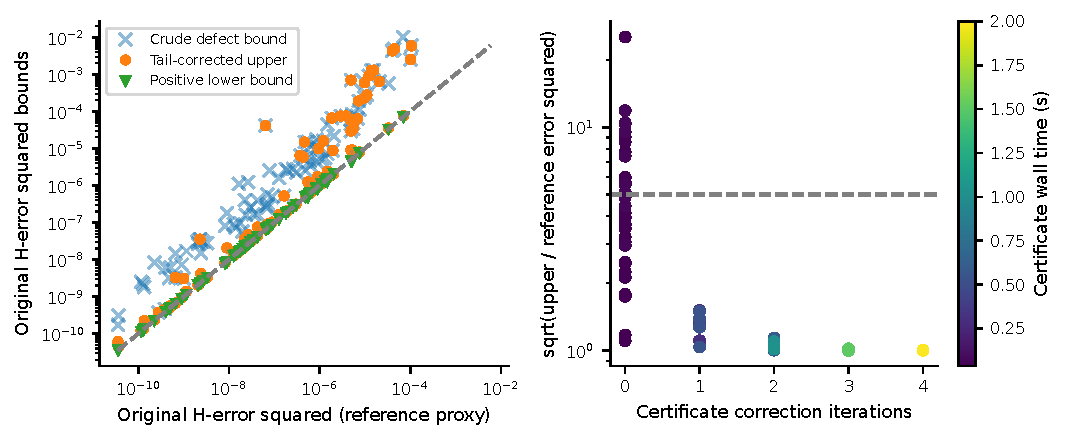
\includegraphics[width=\linewidth]{figures/Figure4_certificate.pdf}
\caption{Conditional local energy-error calibration. Left: squared errors and bounds. Right: upper \(H\)-norm effectivity and paid wall time. Zero lower bounds remain in the data but cannot appear on a logarithmic axis.}
\end{figure}

The separate unpreconditioned eight-action Gauss/Radau diagnostic has 192 action rows. Its conditional bounds are supported by the eligible finite-reference intervals. Final \(H\)-norm effectivity is about 1.005, but the median paired time ratio to accepted B0 is 1.514. It is separately paid offline work, not an extra free consequence of the deployed PCG trajectory.

All E5 routes use the same \(M_0\), full actions, initial proposal, and 99\% reduction target. B1 is a bounded material-history/Krylov adaptation; it compresses accumulated paid step/gradient history by SVD to eight directions and is not a reproduction of a named published solver. B2 is a selective sensitivity/adjoint adaptation, likewise not a full reproduction of adaptive-RB literature. B3 uses paired warm repair; B4 and B5 use paired and generic augmentation respectively. B4/B5 comparisons isolate bank source under the same route; B3/B4 also change execution route.

\begin{table}[tbp]\centering\footnotesize\setlength{\tabcolsep}{3pt}
\begin{tabularx}{\linewidth}{lXXXXX}\toprule
Route & Method-stage ratio [95\% CI] & Anchor-inclusive ratio [95\% CI] & Cold-equivalent ratio [95\% CI] & Median PCG corrections & Median full RHS \\\midrule
B0 & 1 & 1 & 1 & 2 & 66 \\
B1 & 3.489 [3.457, 3.541] & 1.386 [1.248, 1.392] & 1.316 [1.187, 1.320] & 0 & 234 \\
B2 & 2.308 [2.264, 2.321] & 1.199 [1.123, 1.205] & 1.163 [1.093, 1.168] & 2 & 150 \\
B3 & 3.757 [3.528, 4.147] & 1.416 [1.330, 1.445] & 1.341 [1.235, 1.368] & 1 & 342 \\
B4 & 9.786 [9.430, 10.031] & 2.299 [1.908, 2.365] & 2.066 [1.678, 2.121] & 1 & 648 \\
B5 & 9.505 [9.287, 9.753] & 2.270 [1.880, 2.361] & 2.039 [1.657, 2.111] & 1 & 642 \\
\bottomrule\end{tabularx}
\end{table}

The B3 anchor-inclusive ratio is 1.41629, with object-bootstrap interval [1.32959, 1.44545]. Each ratio first pairs the same object, anchor, and repeat with B0; six ratios per object are collapsed by a median, followed by an eight-object median and bootstrap. ``Anchor-inclusive'' is method wall time plus shared ROM setup and full-state anchor time. The cold equivalent additionally allocates common geometry setup across three anchors and must not be summed over methods as actual campaign elapsed time. Offline reference and truth generation are separate.

JVP/VJP call counts alone do not count batched columns. Full RHS counts each full-solve right-hand-side column. Candidate generation, adjoint pullbacks, full \(JZ/HZ\), QR, small solves, and refreshes remain charged. E3 timings omit candidate generation for direct steps and random generation/QR for generic banks, while single-sided tests are charged the shared paired build. Those unequal subtotals cannot support end-to-end claims.

Development measured a 1.9249 s median bank-plus-warm phase and an estimated PCG saving of -0.0762 s after removing that expense. The frozen controller disabled unpaid new banks; held-out timings were not used to learn a new rule. \(M_0\) is rebuilt at each anchor. No verified cross-anchor spectral transfer, dynamic rolling cost adaptation, or N-Port rank-saving result is part of the implemented evidence.

\section*{S8. Nonlinear, noise, and finer-discretization evidence}

Five preselected objects compare B0, B1, static ROM, and MURR. The other three provide B0 trajectories and anchors. All methods share \(\chi_0=0.1+0.04i\), prior weight \(10^{-5}\), initial LM damping 0.01 multiplied by 0.3 every three iterations, an 18-iteration cap, physical projection, and full nonlinear Armijo acceptance. ``Static'' denotes a fixed Gs24 mode-selection rule plus the current primal anchor, with operators refreshed at each state, not a single immutable operator.

The registered endpoint criteria are \(e_{\chi,m}\le1.02e_{\chi,B0}+0.002\) and \(e_{y,m}\le1.02e_{y,B0}+0.0002\). Receiver holdout uses a rotated receiver array at the same frequency and incident fields. This is distinct from object-level holdout from development. A B0 material error above 25\% triggers an insufficient-recovery screen; passing it alone does not prove accurate or generally robust reconstruction.

\begin{table}[tbp]\centering\footnotesize\setlength{\tabcolsep}{3pt}
\begin{tabularx}{\linewidth}{lXXXXXX}\toprule
Object & B0 material error & Static material error & B0 seconds & Static seconds & B0/static state trials & Static endpoint noninferiority \\\midrule
11 & 2.810\% & 3.906\% & 94.7 & 73.4 & 18/18 & fail \\
13 & 0.973\% & 1.135\% & 92.4 & 206.8 & 16/57 & pass \\
15 & 0.447\% & 0.540\% & 101.8 & 140.9 & 18/38 & pass \\
16 & 9.539\% & 16.320\% & 553.5 & 684.8 & 42/64 & fail \\
17 & 0.067\% & 0.128\% & 233.8 & 371.2 & 16/34 & pass \\
\bottomrule\end{tabularx}
\end{table}

MURR follows B0 and has bitwise-identical saved materials in all five objects. Its nonlinear time ratio is 1.000 [0.994, 1.019]. This is a skip-path result, not paired enrichment evidence. Object 16's combined 9.54\% B0/MURR material error contains real-part error 8.38\% and imaginary-part error 36.82\%; the static imaginary error is 50.33\%. Visual loss and boundary errors are retained, not hidden behind the combined norm. A voxel tangent of dimension 5488 with 1536 real measurements has unregularized local Jacobian nullity at least 3952; that dimensional fact is not a global nonlinear nonuniqueness theorem.

\begin{figure}[tbp]\centering
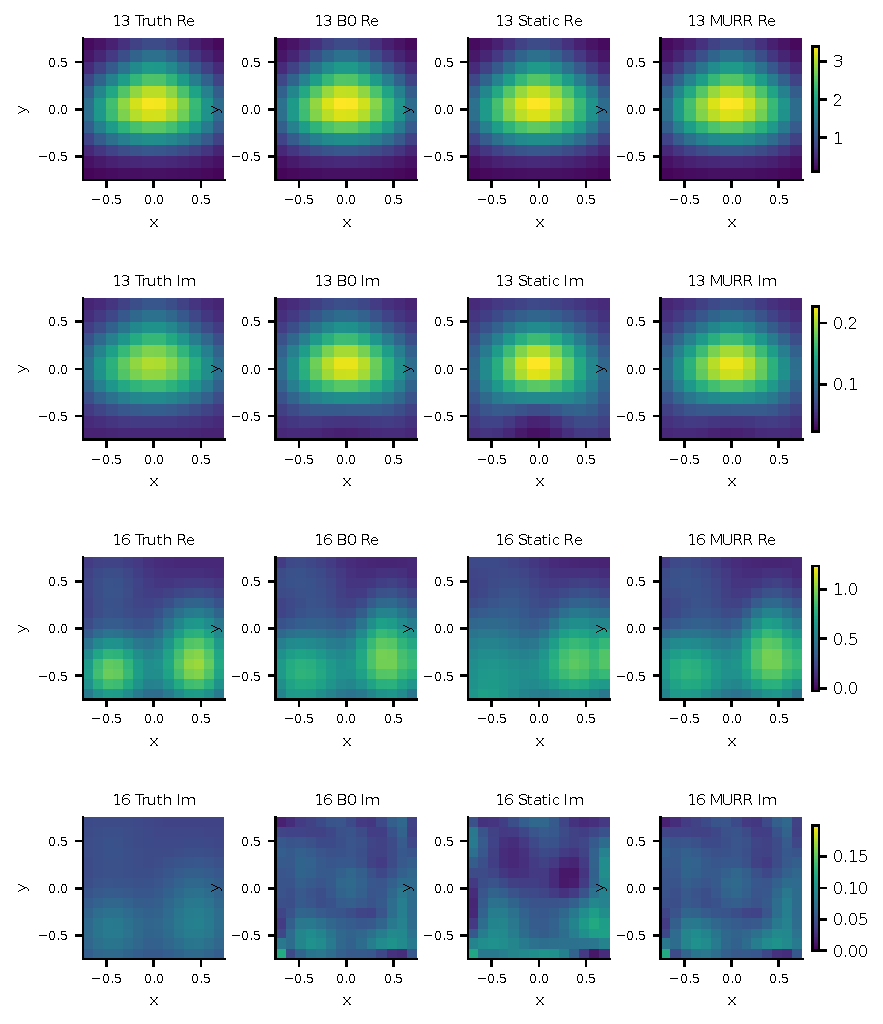
\includegraphics[width=\linewidth]{figures/Figure6_material_slices.pdf}
\caption{Smooth-target material slices on shared row scales for truth, matched full PCG, the fixed current rule, and the cost-controlled skip policy. Object 13 uses finer-grid data; object 16 is same-grid stress. Slices are the positive central cell planes, not exactly \(z=0\). Identity of the full-PCG and skip-policy estimates shows that no paired bank was executed.}
\end{figure}

The full nonlinear B0 trajectories reach as many as 37 PCG corrections as LM damping changes. The fixed-curvature E5 median cannot represent the entire nonlinear solve. Explicit gradient fallbacks, projection distances, and all accepted/rejected full-state trials remain paid.

Two Gaussian objects use one fixed complex noise realization at each nonzero level, shared across B0/MURR. The clean synthetic norm remains the normalization; these are controlled checks, not noise-blind deployment. The shared endpoints are:

\begin{table}[tbp]\centering\footnotesize\setlength{\tabcolsep}{3pt}
\begin{tabularx}{\linewidth}{lXXXXXXX}\toprule
Object & Noise & Material error & Clean receiver-holdout relative error & B0 seconds & Linear certified proposals & Full-state trials & Gradient fallbacks \\\midrule
11 & 0\% & 2.810\% & 0.00005953 & 94.7 & 18/18 & 18 & 0 \\
11 & 1\% & 12.116\% & 0.001587 & 596.5 & 18/18 & 164 & 11 \\
11 & 3\% & 18.879\% & 0.004846 & 631.2 & 18/18 & 175 & 13 \\
13 & 0\% & 0.973\% & 0.0007953 & 92.4 & 16/16 & 16 & 0 \\
13 & 1\% & 1.527\% & 0.001801 & 94.5 & 16/16 & 16 & 0 \\
13 & 3\% & 2.362\% & 0.004622 & 96.5 & 16/16 & 16 & 0 \\
\bottomrule\end{tabularx}
\end{table}

For object 11 at 1\% noise, all 18 preprojection proposals were accepted by the local certificate, but only seven retain that provenance after 11 gradient replacements. At 3\%, five retain it after 13 replacements. Neither count certifies constrained optimality. None of the four nonzero-noise endpoints crosses 25\% material error, but skipped banks establish no paired-bank noise advantage.

The finer-grid endpoint check uses object 13 only. Saved Gaussian coefficients are lifted to \(14^3\) using the same continuous dictionary, with maximum fitting residual \(2.147\times10^{-15}\), followed by forward evaluation only. Exact B0/MURR material identity allows one shared fine solve.

\begin{table}[tbp]\centering\footnotesize\setlength{\tabcolsep}{3pt}
\begin{tabularx}{\linewidth}{lXXXXX}\toprule
Method & Material error at \(12^3\) & Material error at \(14^3\) & Clean holdout at \(12^3\) & Clean holdout at \(14^3\) & Training field at \(14^3\) \\\midrule
B0 / MURR & 0.009734 & 0.009733 & 0.0007953 & 0.007911 & 0.007910 \\
Static & 0.01135 & 0.01134 & 0.0008284 & 0.007947 & 0.007946 \\
\bottomrule\end{tabularx}
\end{table}

All entries are relative norms, not percentages. The 0.7809\% coarse/fine truth-field discrepancy uses the training acquisition and fine truth-field norm. The approximately 0.00361 percentage-point static--B0 fine holdout difference uses the rotated receiver operator and its own truth norm. Their operators and denominators differ; the former is not an error bar or a resolution threshold for the latter. The evaluation reveals discretization dependence without providing a physical-error enclosure for method differences or a rigorous continuum bound from two grids. It was registered after initial held-out inspection, does not alter trajectories or thresholds, and remains within the same DDA family.

\section*{S9. Evidence provenance and final scope}

The original smooth-target campaign ran on an RTX 4060 Laptop GPU, 8 GB, with an i9-14900HX host. Its 20 main jobs and one fine-grid endpoint evaluation completed. Peak GPU allocation/reservation was 5.064/6.074 GiB. A separate development native-process failure with exit code 3221225477 and its successful same-configuration retry remain distinct records; the cause is not inferred from the exit code.

The immutable A12 experiment ledger has 1698 data rows, including 31 process records, 24 anchors, 35 nonlinear records, 576 iteration rows, 648 E3 method rows, 96 calibrations, and 288 E5 executions. It includes development and rejected/failed records; it is not a count of independent held-out experiments. The final writing read all rows and retained the original files.

Three analysis corrections remain essential. First, the legacy zero-valued method-level fallback field is not a count of projected-gradient fallback; per-iteration history is authoritative. Second, history objectives are pre-step while material errors are post-step; final objective is reconstructed from the last accepted trial or unchanged state rather than a rejected last attempt. Third, original linear certification and retained certificate provenance after projection/fallback are distinct events. These corrections affect reporting, not frozen algorithms or measurements.

The feedback, certificate, cost, and smooth-reconstruction figures reuse original data; the mechanism schematic and repair comparison have been redrawn for this manuscript. Corresponding CSV sidecars and per-anchor JSON remain authoritative. Raw figure ratios, empirical table values, finite-reference error intervals, complete histories, and source provenance are linked in the final claim ledger. Earlier conditional cross-anchor, TSOM-safe, and N-Port extensions remain in the historical supplement but are not added as contributions to this mechanism paper.

The manuscript and this supplement state and prove the theoretical results directly. New revision diagnostics are kept separate from the original campaign. The original S-DBIM/FFT-TSOM full-text gaps remain in the final reference audit. Inaccessible text is not evidence that an equivalent result does not exist.

\section*{S10. Precision path in five registered numerical closure failures}

The original 72-pair study registered five normalized closure failures, all at the first state with the TSOM-inspired bank. We retained that decision and replayed those five cases together with three passing controls of the same bank and state index. The original source snapshot fixes the current model; the replay records the hash of its historical TSOM candidate dependency. Current, Schur, and Jacobian actions use \(\texttt{complex128}\); material normal steps and material signatures use \(\texttt{float64}\). No formal reconstruction uses the FP32 diagnostic branch.

Independent calculation of \(s_C\) and \(s_0\), followed by subtraction, gives an absolute closure distance between \(4.48\times10^{-16}\) and \(6.26\times10^{-14}\). The corresponding step changes have \(H\)-norm between \(2.01\times10^{-7}\) and \(5.00\times10^{-5}\). To locate cancellation, the same step difference was evaluated from
\begin{equation}
H_C\Delta s=-\{\Delta J^*r+[J_C^*J_C-J_0^*J_0]s_0\},\qquad\Delta s=s_C-s_0,
\label{eq:stable-step-difference}
\end{equation}
using the low-rank Schur JVP/VJP, without forming a complete voxel Jacobian or a dense material Hessian. The eight direct-subtraction normalized distances range from \(1.42\times10^{-11}\) to \(1.03\times10^{-8}\); the difference-equation distances range from \(2.06\times10^{-15}\) to \(2.48\times10^{-14}\). The small Schur singular values lie in \([1.0624,1.0684]\), its normalized solve backward error is at most \(2.15\times10^{-16}\), and no tracked nonzero FP64 value is subnormal. This is numerical evidence for cancellation in the two-step subtraction followed by division by a small true step change, not for Schur ill-conditioning or underflow.

A controlled small-Schur precision test gives CPU/GPU FP64 solution differences of \(1.17\times10^{-16}\)--\(2.18\times10^{-16}\). GPU FP32 differs from CPU FP64 by \(6.58\times10^{-8}\)--\(1.43\times10^{-7}\), illustrating why changing precision would answer a different question. Complete GPU FP64 replays of the same eight saved anchors give direct-subtraction normalized distances of \(1.10\times10^{-11}\)--\(1.23\times10^{-8}\), versus \(2.17\times10^{-15}\)--\(3.21\times10^{-14}\) from the difference equation; no tracked GPU intermediate is subnormal. The GPU FP32 branch is a small-Schur stress test, not a full inverse replay or the precision used in the original campaign. Original failed labels remain unchanged.

\begin{figure}[tbp]\centering
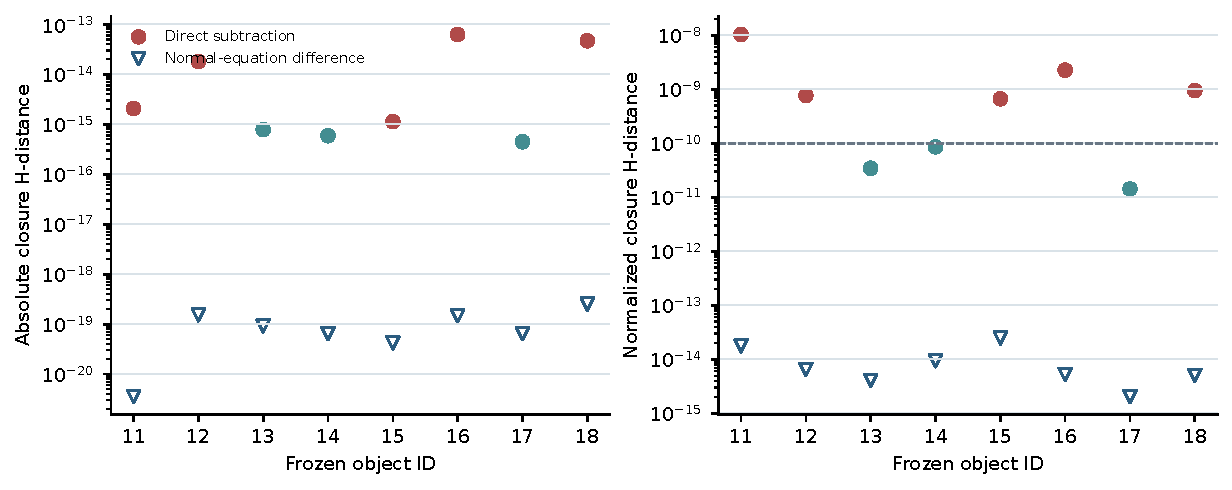
\includegraphics[width=\linewidth]{figures/Figure_precision_cancellation.pdf}
\caption{Targeted CPU FP64 replay of five historical closure failures (red) and three matched passing cases (teal). Directly subtracting independently computed regularized steps leaves small absolute errors that grow after division by the step difference. The Schur-action normal-equation-difference route computes the same quantity without the cancellation. Complete GPU FP64 replay follows the same pattern; its per-case values are tabulated in the R1 raw-data companion. The dashed line is the original \(10^{-10}\) tolerance floor; original status labels are unchanged.}
\end{figure}

\section*{S11. Complete sharp-target primary endpoints}

Table~\ref{tab:sharp-all} lists every completed primary trajectory, including real and imaginary contrast error, fixed-threshold outer-support overlap, held-out response, true objective ratio, fallback events, and counted full Jacobian-vector right-hand sides. The threshold is the predeclared midpoint between zero background and the lowest nonzero real material class; it is used only for evaluation, not supplied as a region to the inverse solver. A dash in the full-JVP column means that the fixed-current route did not perform the corresponding full-model material action. Successful-segment algorithmic time does not erase crashed attempts or restarted setup; campaign occupation is computed from every started job in the remote execution ledger.

\begin{table}[tbp]\centering\caption{Complete frozen sharp-scene primary endpoints. Material errors and IoU are against the declared discrete truth on a common grid. The true objective ratio is final/initial; fallback counts are recorded nonlinear fallback events. Times are successful-segment algorithmic totals including shared setup, not inclusive GPU occupation for failed/retried attempts. Inclusive occupation is separately charged in the run ledger. Re and Im RMSE use contrast units.}\label{tab:sharp-all}
\resizebox{\textwidth}{!}{\begin{tabular}{lllr rrrrrrrrr}\hline
Object & Noise & Method & Re RMSE & Im RMSE & Rel. material & IoU & Held-out & Obj. ratio & Fallback & Accepted & Time (s) & Full JVP RHS \\\hline
sphere & 0\% & full PCG & 1.256 & 0.069 & 0.755 & 0.026 & 0.027 & 0.001109 & 11 & 18 & 427.2 & 9804 \\
sphere & 0\% & fixed Gs24 & 1.275 & 0.061 & 0.766 & 0.000 & 0.032 & 0.001458 & 12 & 18 & 274.1 & -- \\
sphere & 1\% & full PCG & 1.256 & 0.070 & 0.755 & 0.026 & 0.027 & 0.001205 & 11 & 18 & 432.7 & 9960 \\
sphere & 1\% & fixed Gs24 & 1.270 & 0.061 & 0.764 & 0.000 & 0.032 & 0.001605 & 11 & 18 & 246.3 & -- \\
split cuboid & 0\% & full PCG & 1.000 & 0.071 & 0.750 & 0.455 & 0.047 & 0.003368 & 14 & 18 & 479.7 & 9180 \\
split cuboid & 0\% & fixed Gs24 & 1.009 & 0.081 & 0.757 & 0.437 & 0.055 & 0.004693 & 14 & 18 & 274.6 & -- \\
split cuboid & 1\% & full PCG & 0.999 & 0.070 & 0.749 & 0.457 & 0.047 & 0.003499 & 14 & 18 & 226.7 & 5826 \\
split cuboid & 1\% & fixed Gs24 & 1.008 & 0.079 & 0.757 & 0.439 & 0.055 & 0.004861 & 14 & 18 & 267.6 & -- \\
eccentric shell & 0\% & full PCG & 0.836 & 0.059 & 0.560 & 0.692 & 0.019 & 0.0005275 & 8 & 18 & 356.4 & 8400 \\
eccentric shell & 0\% & fixed Gs24 & 0.875 & 0.078 & 0.587 & 0.675 & 0.026 & 0.00101 & 11 & 18 & 228.0 & -- \\
eccentric shell & 1\% & full PCG & 0.869 & 0.072 & 0.583 & 0.662 & 0.021 & 0.0008201 & 11 & 18 & 418.6 & 9156 \\
eccentric shell & 1\% & fixed Gs24 & 0.874 & 0.076 & 0.586 & 0.672 & 0.026 & 0.001155 & 11 & 18 & 236.1 & -- \\
two ellipsoids & 0\% & full PCG & 1.086 & 0.053 & 0.906 & 0.000 & 0.073 & 0.01224 & 15 & 18 & 462.7 & 9012 \\
two ellipsoids & 0\% & fixed Gs24 & 1.079 & 0.055 & 0.901 & 0.000 & 0.072 & 0.01177 & 13 & 18 & 301.7 & -- \\
two ellipsoids & 1\% & full PCG & 1.087 & 0.053 & 0.907 & 0.000 & 0.072 & 0.01208 & 15 & 18 & 464.9 & 9108 \\
two ellipsoids & 1\% & fixed Gs24 & 1.079 & 0.055 & 0.901 & 0.000 & 0.071 & 0.0116 & 14 & 18 & 288.5 & -- \\
\hline\end{tabular}}
\end{table}


Table~\ref{tab:sharp-class-means} makes the contrast loss explicit. These class averages are evaluation summaries at the true class locations, not class labels supplied to the inverse solver. In particular, the high-contrast ellipsoid's recovered mean is less than one in real contrast for both methods although its true value is seven.

\begin{table}[tbp]\centering\caption{Zero-noise nonbackground class-mean complex contrast, evaluated on the true class locations without revealing regions to the inverse solver. Values in parentheses are real and imaginary parts.}\label{tab:sharp-class-means}
\begin{tabular}{llrrr}\hline
Object & Class & True (Re,Im) & Full PCG & Fixed Gs24 \\\hline
sphere & 1 & (5.0,0.2) & (1.909,0.062) & (1.820,0.064) \\
split cuboid & 1 & (3.0,0.1) & (1.401,0.041) & (1.361,0.035) \\
split cuboid & 2 & (5.0,0.2) & (1.659,0.027) & (1.600,0.019) \\
eccentric shell & 1 & (3.0,0.1) & (1.875,0.045) & (1.773,0.051) \\
eccentric shell & 2 & (7.0,0.3) & (3.731,0.204) & (3.438,0.133) \\
two ellipsoids & 1 & (3.0,0.1) & (0.509,0.008) & (0.506,0.004) \\
two ellipsoids & 2 & (7.0,0.3) & (0.781,0.011) & (0.833,0.012) \\
\hline\end{tabular}
\end{table}


The complete predeclared 3\% noise and same-grid resolution extensions appear in Table~\ref{tab:sharp-extension}; they are distinct from the primary 16 trajectories and the historical local 72 comparisons.

\begin{table}[tbp]\centering\caption{All eight predeclared sharp-scene extension endpoints, separate from the 16 primary trajectories. The 3\% noise rows use the main 12-cell inverse grid and 14-cell truth grid. The resolution rows fit 14-cell data on the same 14-cell inverse grid, so they are not independent discretization checks. Material and IoU are against the declared discrete truth; times exclude failed/restarted attempts, which remain in the GPU occupation ledger.}\label{tab:sharp-extension}
\resizebox{\textwidth}{!}{\begin{tabular}{llllrrrrr}\hline
Object & Extension & Grid & Method & Rel. material & IoU & Held-out & Obj. ratio & Time (s) \\\hline
sphere & resolution & 14 & full PCG & 0.7206 & 0.0263 & 0.02673 & 0.00106 & 1010.4 \\
sphere & resolution & 14 & fixed Gs24 & 0.7366 & 0.0000 & 0.03131 & 0.001438 & 779.7 \\
split cuboid & 3\% noise & 12 & full PCG & 0.7501 & 0.4583 & 0.04666 & 0.004603 & 462.8 \\
split cuboid & 3\% noise & 12 & fixed Gs24 & 0.7584 & 0.4341 & 0.05483 & 0.005939 & 256.2 \\
split cuboid & resolution & 14 & full PCG & 0.7153 & 0.5980 & 0.05268 & 0.004304 & 1115.6 \\
split cuboid & resolution & 14 & fixed Gs24 & 0.7191 & 0.5359 & 0.05479 & 0.004654 & 779.2 \\
eccentric shell & 3\% noise & 12 & full PCG & 0.5830 & 0.6703 & 0.02454 & 0.002 & 410.9 \\
eccentric shell & 3\% noise & 12 & fixed Gs24 & 0.5845 & 0.6768 & 0.02710 & 0.002253 & 224.6 \\
\hline\end{tabular}}
\end{table}


At the 12 saved zero-noise full-model pre-update states, three candidate-bank rules provide the 36 local rows in Tables~\ref{tab:sharp-local-gains} and \ref{tab:sharp-local-mechanism}. Every paired and material Krylov space has equal real rank 48. The same-state bank rows share the full physical state and cannot be counted as independent targets. Negative direct gain means that the new current model's step is worse on the unchanged full quadratic than the previous reduced-model step.

% Generated from results/local_updates/S*_anchor*.json; do not edit by hand.
% Complete: 4 scenes x 3 frozen anchors x 3 candidate banks = 36 rows.
\begin{table*}[tbp]\centering\scriptsize\setlength{\tabcolsep}{3pt}
\caption{Frozen sharp-scene local update comparisons, part I. Gains are reductions in the same full regularized quadratic relative to the old current-model step; negative values mean an increase. The shared rank column is the equal real material rank of paired and Krylov. These are specified current-bank diagnostics, not nonlinear paired trajectories. All 36 scene--anchor--bank rows are retained.}\label{tab:sharp-local-gains}
\begin{tabular}{ll l r r r r r}\toprule
Scene & Anchor & Bank & Current cols. & Both ranks & Direct gain & Paired gain & Krylov gain\\\midrule
Sphere & 0 & Residual & 2 & 48 & $1.029\!\times\!10^{-4}$ & $1.376\!\times\!10^{-4}$ & $1.704\!\times\!10^{-4}$\\
Sphere & 0 & Gs & 2 & 48 & $-1.722\!\times\!10^{-6}$ & $7.888\!\times\!10^{-5}$ & $1.704\!\times\!10^{-4}$\\
Sphere & 0 & TSOM-inspired & 2 & 48 & $9.032\!\times\!10^{-8}$ & $7.948\!\times\!10^{-5}$ & $1.704\!\times\!10^{-4}$\\
Sphere & 3 & Residual & 2 & 48 & $3.328\!\times\!10^{-4}$ & $5.153\!\times\!10^{-4}$ & $6.449\!\times\!10^{-4}$\\
Sphere & 3 & Gs & 2 & 48 & $2.702\!\times\!10^{-5}$ & $1.752\!\times\!10^{-4}$ & $6.449\!\times\!10^{-4}$\\
Sphere & 3 & TSOM-inspired & 2 & 48 & $2.920\!\times\!10^{-6}$ & $3.193\!\times\!10^{-4}$ & $6.449\!\times\!10^{-4}$\\
Sphere & 7 & Residual & 2 & 48 & $1.377\!\times\!10^{-4}$ & $3.327\!\times\!10^{-4}$ & $4.639\!\times\!10^{-4}$\\
Sphere & 7 & Gs & 2 & 48 & $2.977\!\times\!10^{-5}$ & $2.059\!\times\!10^{-4}$ & $4.639\!\times\!10^{-4}$\\
Sphere & 7 & TSOM-inspired & 2 & 48 & $2.693\!\times\!10^{-6}$ & $1.996\!\times\!10^{-4}$ & $4.639\!\times\!10^{-4}$\\
Split cuboid & 0 & Residual & 2 & 48 & $1.130\!\times\!10^{-4}$ & $2.386\!\times\!10^{-4}$ & $2.674\!\times\!10^{-4}$\\
Split cuboid & 0 & Gs & 2 & 48 & $1.063\!\times\!10^{-5}$ & $1.357\!\times\!10^{-4}$ & $2.674\!\times\!10^{-4}$\\
Split cuboid & 0 & TSOM-inspired & 2 & 48 & $2.002\!\times\!10^{-7}$ & $1.198\!\times\!10^{-4}$ & $2.674\!\times\!10^{-4}$\\
Split cuboid & 3 & Residual & 2 & 48 & $2.227\!\times\!10^{-4}$ & $4.640\!\times\!10^{-4}$ & $8.773\!\times\!10^{-4}$\\
Split cuboid & 3 & Gs & 2 & 48 & $1.582\!\times\!10^{-5}$ & $3.193\!\times\!10^{-4}$ & $8.773\!\times\!10^{-4}$\\
Split cuboid & 3 & TSOM-inspired & 2 & 48 & $1.130\!\times\!10^{-5}$ & $3.688\!\times\!10^{-4}$ & $8.773\!\times\!10^{-4}$\\
Split cuboid & 7 & Residual & 2 & 48 & $3.396\!\times\!10^{-4}$ & $5.152\!\times\!10^{-4}$ & $8.438\!\times\!10^{-4}$\\
Split cuboid & 7 & Gs & 2 & 48 & $-1.682\!\times\!10^{-5}$ & $2.292\!\times\!10^{-4}$ & $8.438\!\times\!10^{-4}$\\
Split cuboid & 7 & TSOM-inspired & 2 & 48 & $1.014\!\times\!10^{-5}$ & $3.049\!\times\!10^{-4}$ & $8.438\!\times\!10^{-4}$\\
Eccentric shell & 0 & Residual & 2 & 48 & $1.237\!\times\!10^{-4}$ & $1.665\!\times\!10^{-4}$ & $1.934\!\times\!10^{-4}$\\
Eccentric shell & 0 & Gs & 2 & 48 & $5.855\!\times\!10^{-6}$ & $1.009\!\times\!10^{-4}$ & $1.934\!\times\!10^{-4}$\\
Eccentric shell & 0 & TSOM-inspired & 2 & 48 & $1.200\!\times\!10^{-7}$ & $9.779\!\times\!10^{-5}$ & $1.934\!\times\!10^{-4}$\\
Eccentric shell & 3 & Residual & 2 & 48 & $3.116\!\times\!10^{-4}$ & $4.230\!\times\!10^{-4}$ & $5.712\!\times\!10^{-4}$\\
Eccentric shell & 3 & Gs & 2 & 48 & $3.109\!\times\!10^{-5}$ & $1.545\!\times\!10^{-4}$ & $5.712\!\times\!10^{-4}$\\
Eccentric shell & 3 & TSOM-inspired & 2 & 48 & $2.774\!\times\!10^{-8}$ & $2.928\!\times\!10^{-4}$ & $5.712\!\times\!10^{-4}$\\
Eccentric shell & 7 & Residual & 2 & 48 & $2.243\!\times\!10^{-4}$ & $3.017\!\times\!10^{-4}$ & $3.547\!\times\!10^{-4}$\\
Eccentric shell & 7 & Gs & 2 & 48 & $1.578\!\times\!10^{-5}$ & $1.884\!\times\!10^{-4}$ & $3.547\!\times\!10^{-4}$\\
Eccentric shell & 7 & TSOM-inspired & 2 & 48 & $2.518\!\times\!10^{-6}$ & $1.902\!\times\!10^{-4}$ & $3.547\!\times\!10^{-4}$\\
Two ellipsoids & 0 & Residual & 2 & 48 & $2.509\!\times\!10^{-4}$ & $3.901\!\times\!10^{-4}$ & $4.616\!\times\!10^{-4}$\\
Two ellipsoids & 0 & Gs & 2 & 48 & $6.357\!\times\!10^{-5}$ & $2.687\!\times\!10^{-4}$ & $4.616\!\times\!10^{-4}$\\
Two ellipsoids & 0 & TSOM-inspired & 2 & 48 & $2.026\!\times\!10^{-8}$ & $2.195\!\times\!10^{-4}$ & $4.616\!\times\!10^{-4}$\\
Two ellipsoids & 3 & Residual & 2 & 48 & $5.221\!\times\!10^{-4}$ & $6.465\!\times\!10^{-4}$ & $8.541\!\times\!10^{-4}$\\
Two ellipsoids & 3 & Gs & 2 & 48 & $2.940\!\times\!10^{-6}$ & $3.777\!\times\!10^{-4}$ & $8.541\!\times\!10^{-4}$\\
Two ellipsoids & 3 & TSOM-inspired & 2 & 48 & $5.350\!\times\!10^{-6}$ & $3.086\!\times\!10^{-4}$ & $8.541\!\times\!10^{-4}$\\
Two ellipsoids & 7 & Residual & 2 & 48 & $6.328\!\times\!10^{-4}$ & $7.438\!\times\!10^{-4}$ & $9.726\!\times\!10^{-4}$\\
Two ellipsoids & 7 & Gs & 2 & 48 & $6.172\!\times\!10^{-5}$ & $5.108\!\times\!10^{-4}$ & $9.726\!\times\!10^{-4}$\\
Two ellipsoids & 7 & TSOM-inspired & 2 & 48 & $1.998\!\times\!10^{-5}$ & $4.070\!\times\!10^{-4}$ & $9.726\!\times\!10^{-4}$\\
\bottomrule\end{tabular}\end{table*}

\begin{table*}[tbp]\centering\scriptsize\setlength{\tabcolsep}{5pt}
\caption{Frozen sharp-scene local update comparisons, part II. Closure distance is the absolute and normalized \(H\)-norm distance from the specified enlarged-model step change to the paired material envelope. Feedback/direct is the norm of retained feedback output divided by the norm of raw candidate output for the same bank; the implementation guards the denominator by \(10^{-300}\). Thus an extreme ratio with nearly dark direct output needs its absolute norms for interpretation.}\label{tab:sharp-local-mechanism}
\begin{tabular}{ll l r r r}\toprule
Scene & Anchor & Bank & Closure abs. & Closure rel. & Feedback/direct\\\midrule
Sphere & 0 & Residual & $1.633\!\times\!10^{-14}$ & $1.572\!\times\!10^{-12}$ & $0.694$\\
Sphere & 0 & Gs & $2.325\!\times\!10^{-14}$ & $8.083\!\times\!10^{-12}$ & $0.0806$\\
Sphere & 0 & TSOM-inspired & $3.647\!\times\!10^{-14}$ & $1.264\!\times\!10^{-10}$ & $0.4$\\
Sphere & 3 & Residual & $1.409\!\times\!10^{-14}$ & $8.177\!\times\!10^{-13}$ & $4.92$\\
Sphere & 3 & Gs & $1.262\!\times\!10^{-14}$ & $2.090\!\times\!10^{-12}$ & $0.311$\\
Sphere & 3 & TSOM-inspired & $1.271\!\times\!10^{-14}$ & $1.758\!\times\!10^{-11}$ & $5.26$\\
Sphere & 7 & Residual & $4.434\!\times\!10^{-14}$ & $3.328\!\times\!10^{-12}$ & $5.85$\\
Sphere & 7 & Gs & $4.372\!\times\!10^{-14}$ & $6.415\!\times\!10^{-12}$ & $0.233$\\
Sphere & 7 & TSOM-inspired & $4.426\!\times\!10^{-14}$ & $5.697\!\times\!10^{-11}$ & $6.26$\\
Split cuboid & 0 & Residual & $3.486\!\times\!10^{-14}$ & $2.449\!\times\!10^{-12}$ & $0.769$\\
Split cuboid & 0 & Gs & $4.244\!\times\!10^{-14}$ & $1.124\!\times\!10^{-11}$ & $0.0806$\\
Split cuboid & 0 & TSOM-inspired & $4.908\!\times\!10^{-14}$ & $1.097\!\times\!10^{-10}$ & $0.4$\\
Split cuboid & 3 & Residual & $3.246\!\times\!10^{-14}$ & $1.471\!\times\!10^{-12}$ & $4.18$\\
Split cuboid & 3 & Gs & $2.557\!\times\!10^{-14}$ & $6.334\!\times\!10^{-12}$ & $0.232$\\
Split cuboid & 3 & TSOM-inspired & $2.996\!\times\!10^{-14}$ & $1.934\!\times\!10^{-11}$ & $5.35$\\
Split cuboid & 7 & Residual & $4.054\!\times\!10^{-14}$ & $1.706\!\times\!10^{-12}$ & $4.31$\\
Split cuboid & 7 & Gs & $4.438\!\times\!10^{-14}$ & $1.121\!\times\!10^{-11}$ & $0.215$\\
Split cuboid & 7 & TSOM-inspired & $4.263\!\times\!10^{-14}$ & $1.923\!\times\!10^{-11}$ & $5.61$\\
Eccentric shell & 0 & Residual & $2.130\!\times\!10^{-14}$ & $1.928\!\times\!10^{-12}$ & $0.792$\\
Eccentric shell & 0 & Gs & $2.330\!\times\!10^{-14}$ & $8.565\!\times\!10^{-12}$ & $0.0806$\\
Eccentric shell & 0 & TSOM-inspired & $3.220\!\times\!10^{-14}$ & $1.375\!\times\!10^{-10}$ & $0.4$\\
Eccentric shell & 3 & Residual & $1.703\!\times\!10^{-14}$ & $8.501\!\times\!10^{-13}$ & $5.85$\\
Eccentric shell & 3 & Gs & $1.635\!\times\!10^{-14}$ & $4.310\!\times\!10^{-12}$ & $0.285$\\
Eccentric shell & 3 & TSOM-inspired & $1.714\!\times\!10^{-14}$ & $2.117\!\times\!10^{-11}$ & $5.36$\\
Eccentric shell & 7 & Residual & $3.939\!\times\!10^{-14}$ & $2.654\!\times\!10^{-12}$ & $11.2$\\
Eccentric shell & 7 & Gs & $3.791\!\times\!10^{-14}$ & $1.305\!\times\!10^{-11}$ & $0.227$\\
Eccentric shell & 7 & TSOM-inspired & $4.457\!\times\!10^{-14}$ & $8.323\!\times\!10^{-11}$ & $6.1$\\
Two ellipsoids & 0 & Residual & $1.449\!\times\!10^{-13}$ & $7.450\!\times\!10^{-12}$ & $0.749$\\
Two ellipsoids & 0 & Gs & $2.435\!\times\!10^{-13}$ & $3.514\!\times\!10^{-11}$ & $0.0806$\\
Two ellipsoids & 0 & TSOM-inspired & $2.202\!\times\!10^{-13}$ & $3.136\!\times\!10^{-10}$ & $0.4$\\
Two ellipsoids & 3 & Residual & $1.374\!\times\!10^{-13}$ & $3.890\!\times\!10^{-12}$ & $2.72$\\
Two ellipsoids & 3 & Gs & $1.524\!\times\!10^{-13}$ & $3.744\!\times\!10^{-11}$ & $0.173$\\
Two ellipsoids & 3 & TSOM-inspired & $1.280\!\times\!10^{-13}$ & $6.069\!\times\!10^{-11}$ & $1.93$\\
Two ellipsoids & 7 & Residual & $6.368\!\times\!10^{-13}$ & $1.420\!\times\!10^{-11}$ & $3.04$\\
Two ellipsoids & 7 & Gs & $6.411\!\times\!10^{-13}$ & $8.630\!\times\!10^{-11}$ & $0.169$\\
Two ellipsoids & 7 & TSOM-inspired & $5.961\!\times\!10^{-13}$ & $2.320\!\times\!10^{-10}$ & $1.97$\\
\bottomrule\end{tabular}\end{table*}


\begin{figure*}[tbp]\centering
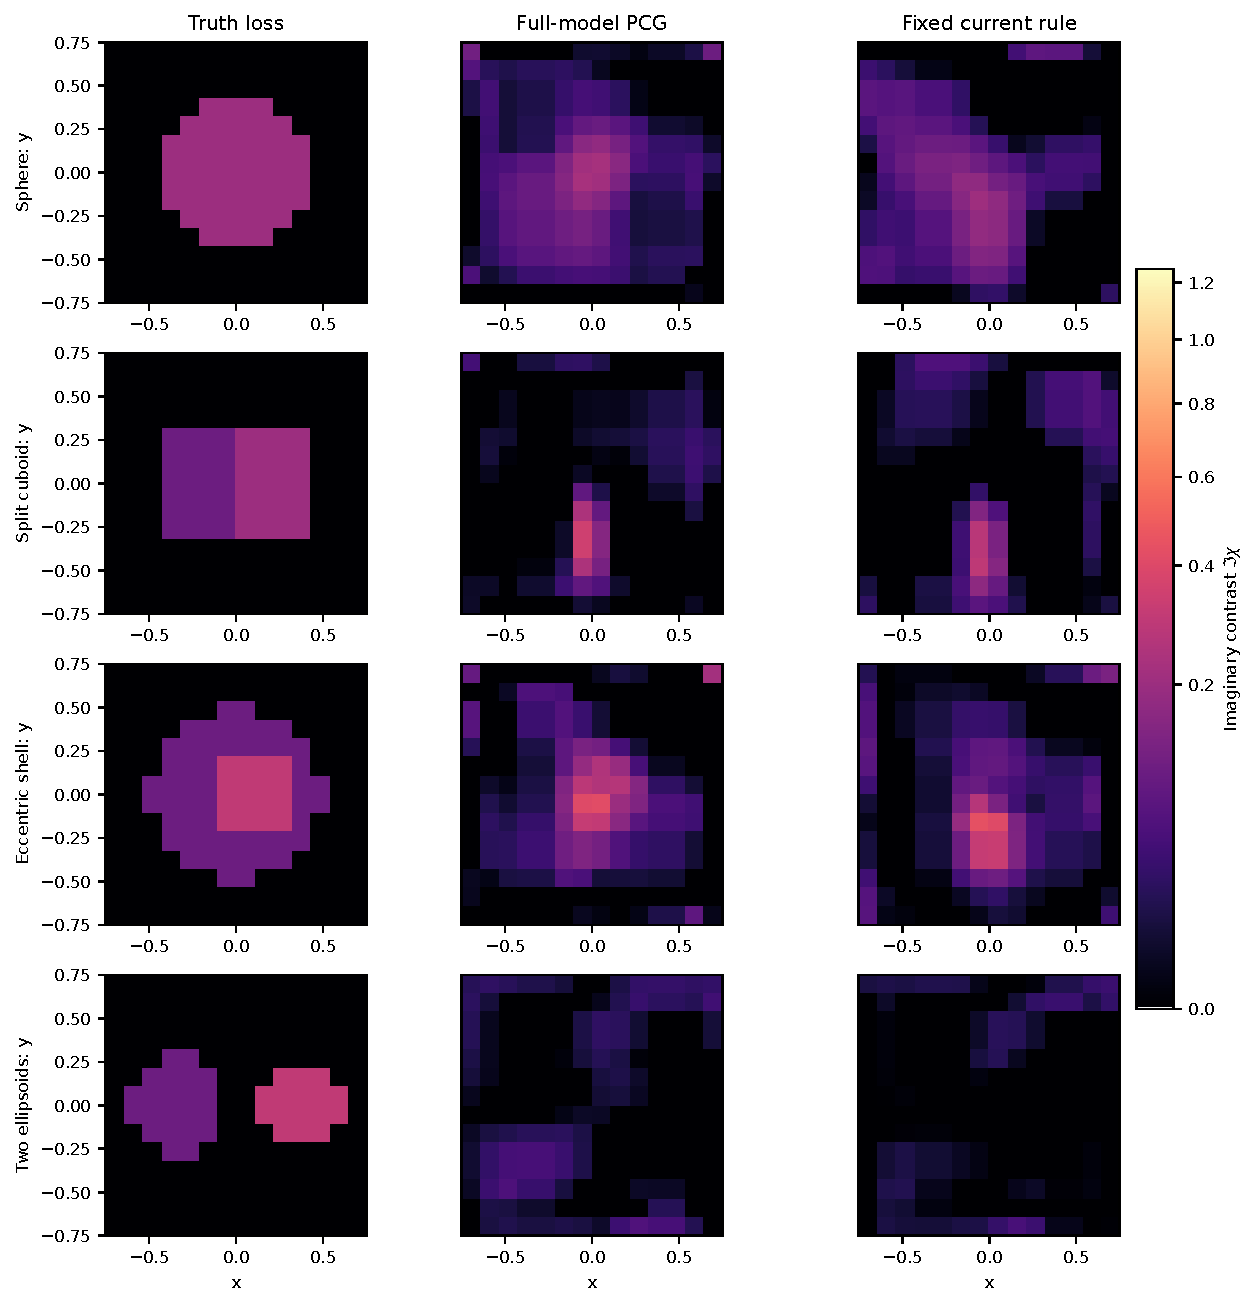
\includegraphics[width=0.94\textwidth]{figures/Figure_sharp_imag_slices.pdf}
\caption{Imaginary-contrast (loss) slices for the four zero-noise sharp targets: sampled truth, full-model PCG, and the fixed Gs24 current-selection rule. Both inversion routes produce diffuse loss and localized high-loss hotspots that do not reproduce the piecewise-constant truth. All panels share one \(\operatorname{PowerNorm}(\gamma=0.45)\) mapping and one physical-value color scale, so displayed brightness is nonlinear in imaginary contrast. The display makes small positive values visible; quantitative real and imaginary errors remain in Table~\ref{tab:sharp-all}. Appearance alone does not quantify material recovery or identify a unique error mechanism.}
\label{fig:sharp-imag-slices}
\end{figure*}

\clearpage
\section*{S12. Receiver-dependent local repair gains}

Table~\ref{tab:faemis-repair} reports the fixed-probe, fixed-absolute-noise synthetic residual experiment described in the main text. The material state and current bank are fixed within each three-radius series, but each receiver defines its own full local quadratic. Paired and Krylov material ranks are both 48 in every row. These are two states with correlated receiver changes, not twelve independent inverse problems. Far-field replacement is not ordered in gain across the two states.

\begin{table}[tbp]\centering\caption{Local full-quadratic gain under finite-distance and strict far-field receiver operators. The far/finite ratio refers to paired gain; Krylov is an equal-real-rank material correction under the same receiver and local quadratic.}\label{tab:faemis-repair}
\resizebox{\textwidth}{!}{\begin{tabular}{llrrrr}\hline
State & Radius & Finite paired & Finite Krylov & Far paired & Far/finite paired \\\hline
Sharp voxel & 5 & 0.0025299 & 0.0065130 & 0.0026130 & 1.0328\\
Sharp voxel & 10 & 0.0011306 & 0.0026628 & 0.0011792 & 1.0430\\
Sharp voxel & 20 & 0.00046452 & 0.0010354 & 0.00047462 & 1.0217\\
Smooth Gaussian & 5 & 0.000055429 & 0.000057983 & 0.000051556 & 0.9301\\
Smooth Gaussian & 10 & 0.000022031 & 0.000024835 & 0.000020807 & 0.9444\\
Smooth Gaussian & 20 & 0.0000058438 & 0.0000068420 & 0.0000054876 & 0.9391\\
\hline\end{tabular}}
\end{table}

\section*{S13. Paid GPU occupation and phase profiling}

The revision consumed 3.416 charged GPU-job hours: 3.140 hours for sharp-target trajectories, 0.083 hours for precision/receiver diagnostics, and 0.192 hours for frozen local comparisons. Three sharp-trajectory and two local-comparison attempts failed before successful retries; their time remains in the occupation total. All 24 planned sharp trajectories (16 primary plus eight declared extensions) and all 12 frozen local-state jobs completed. The largest one-second sampled device-memory fraction was 65.2\% across 12148 samples in 45 trace files; no 80\% warning or 90\% memory stop was recorded. This sampled maximum is not an upper bound on subsecond memory peaks.

At the representative zero-noise full-model sphere, cuboid, and shell trajectories, median per-iteration preparation times were 0.336, 0.328, and 0.320\,s; controller times were 7.773, 6.937, and 5.320\,s; line-search times were 14.617, 20.063, and 4.657\,s. Across 36 candidate banks in the local comparisons, the median candidate generation and two-sided envelope construction were 0.024 and 0.234\,s, respectively; the recorded paired-bank build median was 0.267\,s. The complete diagnostic, including direct current enlargement, paired and Krylov corrections, and full-goal checks, took a median 45.081\,s across 12 saved states. These component medians cannot be added to reconstruct one specific job. They are profiling of distinct workflows, not a new matched-quality paired versus PCG cost comparison. The historical 1.416 anchor-inclusive wall ratio remains the relevant measured method comparison.

\begin{figure*}[tbp]\centering
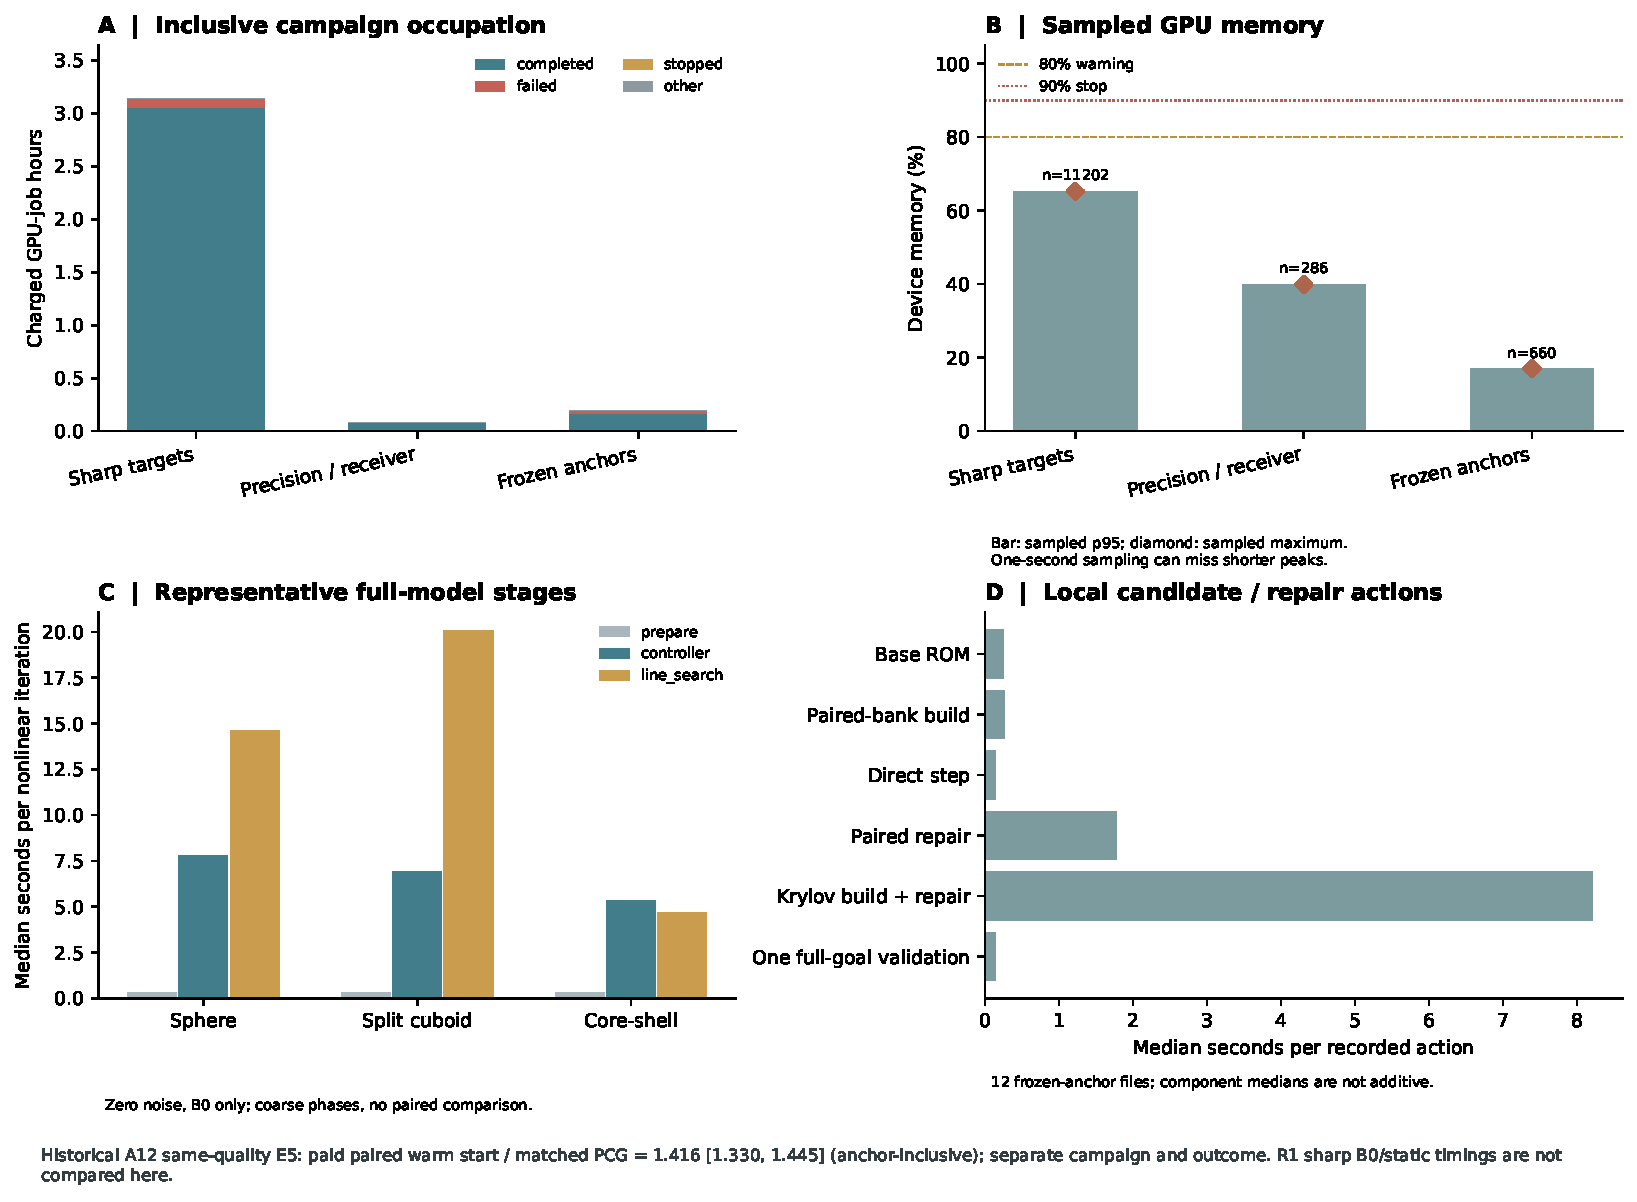
\includegraphics[width=0.96\textwidth]{figures/Figure_cost_resources.pdf}
\caption{Inclusive GPU occupation, sampled device memory, representative full-model nonlinear stages, and frozen-anchor local comparison actions. Failed attempts and retries are charged in panel (a). Panel (b) shows one-second sampled values; it cannot resolve shorter peaks. Panel (c) profiles the full-model baseline, whereas panel (d) combines separate local comparison actions and is not a matched nonlinear solver cost test. The historical paid paired/PCG wall ratio is 1.416 in a separate campaign.}
\label{fig:cost-resources}
\end{figure*}

\clearpage
\section*{S14. Full-material preconditioner execution}
The observation and injection factors also determine a low-rank change of the material normal matrix. This section follows that change into an inverse used by full-H PCG, then records the checks and costs of its implementation. The final solve continues to use the complete material operator.
The new experiments reuse historical states and preserve their original material fields, damping, data, acquisition, and material parameterization. All material coordinates use the declared volume-weighted physical metric. Complex dielectric increments are packed into real and imaginary parts; because the frozen DDA derivative is complex-linear in the increment, the implementation uses its equivalent complex representation internally. The requested two-column current enrichment is a complex current rank, not a two-dimensional real material repair. Over six illuminations, the update signatures may have many more material columns.

Gate 0 compares a dense inverse, an indefinite Woodbury realization, and rank-revealing QR followed by a small SPD solve. Seven cases include random complex matrices, exact and near rank loss, adjoint and realification checks, and a 27-cell vector DDA. The largest small-DDA inverse residual is approximately \(6.3\times10^{-13}\). A separate adapter check uses the production tangent convention for Gaussian and voxel coordinates, with discrepancies below \(3\times10^{-15}\). These are implementation checks, not continuum validation.

Let \(D=Y_bT_b\). The signature-based identity
\[
H_C-H_0=[J_0^*Y_b,T_b^*]
\begin{bmatrix}0&I\\I&Y_b^*Y_b\end{bmatrix}
[J_0^*Y_b,T_b^*]^*
\]
uses block-diagonal observation factors for different illuminations and a shared material coordinate. The small inverse does not evaluate full \(JZ\) or \(HZ\). Its setup still includes candidate projection/SVD, \(LC\), local injection adjoints, whitening by the baseline inverse, and a small Cholesky factorization. An independently built enlarged Galerkin model checks the resulting Jacobian and inverse. These reconstruction checks are offline validation: their costs appear in job occupation, not in the marginal solver comparison.

Every full-H solve starts at the same old-model step. The stopping target is
\[
\frac{\|Hs+h\|_2}{\|h\|_2}\le10^{-8},
\]
with a maximum of 150 PCG iterations and an explicitly recomputed final residual. Each full normal action entails six primal and six adjoint full-wave right-hand sides. The initial and final residual evaluations are charged. No dense full-H factorization is used by the online solver. Baseline timings include CPU copies that retain the first six paid current/material actions; their instrumentation overhead is not separately attributed. Thus the reported wall ratios concern this instrumented prototype, and small single-replay margins cannot establish production acceleration. Exact small-tangent spectra, reference intervals, and the separate 30-step and 100-step voxel Ritz diagnostic are offline data.

A computable conservative energy-error interval follows from \(H\succeq\lambda I\):
\[
\|s-s_*\|_H\le\|Hs+h\|_2/\sqrt\lambda,
\qquad \Phi(s)-\Phi(s_*)\le\|Hs+h\|_2^2/(2\lambda).
\]
The CSV uses an upper bound for \(\|h\|\) obtained from the stored initial full-H action and initial defect. This can be conservative; it is not labeled an exact reference error.

\section*{S15. Probabilistic certificates and reuse accounting}
The bidirectional tail gives a sufficient spectral condition; evaluating it cheaply requires a separate statistical check. Independent receiver/material actions probe the omitted transfer, with an explicit failure probability. We then account for how checking, construction, and history acquisition affect repeated use of the inverse.
For a fixed real operator \(A\) and independent standard real Gaussian vectors \(g_i\),
\[
\Pr\{\|A\|_2>2\max_{1\le i\le8}\|Ag_i\|_2\}
\le[2\Phi_{\rm N}(1/2)-1]^8=4.62285\times10^{-4}.
\]
The primary campaign uses \(A=(J-J_C)\Lambda^{-1/2}\). Its upper bound also bounds \(\eta_C\), but can be loose. All candidates are frozen before these validation probes. A union bound over the 72 candidate checks is 0.0333; sharing probe vectors across fixed banks does not require cross-bank independence for this union bound. One nonvacuous upper bound is not evidence that the other bounds failed probabilistically: a value above one simply gives no contraction certificate.

A post-primary four-case check replaces $\Lambda$ whitening by the available exact $H_C$ inverse factor in the Jacobian probe operator. For prior-adjoint ranks 2/12, the two objects yield upper bounds 3.765/2.342 and 14.345/8.861. All remain vacuous; the factor and probe costs are recorded. These results exclude an easy resolution merely by changing the whitening.

The reuse check factors \(M_{C,a}=FF^*\) and probes the symmetric operator
\[
A=F^*(H_t-H_{C,a})F.
\]
An upper bound below one yields spectral equivalence; the declared refresh threshold is 0.6. The small factor is constructed from the positive eigenvalues of the QR-SPD block, with no hidden regularization. Eight full-H actions per check are charged. A certificate based on a mean-square probe statistic would not satisfy the stated maximum-probe probability formula and is not used.

Chronological policies are always refresh, never refresh, refresh every two saved states, and independent-probe-triggered refresh. Cached construction timings are recharged at each simulated refresh, so the reported totals are measured phase sums, not uninterrupted end-to-end trajectories. At the first state, no historical adjoint bank exists; the reuse driver records a residual-current fallback. Later adjoint banks use previous-state paid current snapshots.

The frozen-H multiple-RHS experiment uses eight distinct one-percent complex measurement-noise realizations at the same late material state. It represents repeated local uncertainty/data-perturbation solves, not eight nonlinear reconstructions. Full state, baseline inverse, and the corresponding RHS construction are genuinely common. Snapshot acquisition is available from the disclosed preceding full solve; it is not a free cold-start resource. The setup and one probabilistic check are paid before the eight proposed solves. Baseline/proposed order alternates.

The initial rank-two material-recycling control receives already-paid histories from separately timed baseline solves. It is therefore an externally assisted historical-information comparator, not a standalone recycling policy. The rank-12 extension corrects this deployment distinction: after the common initial history, each recycling solve captures its own full-H actions and reuses only those. Both controls use a refreshed material coarse correction followed by full-H PCG. Neither is claimed to exhaust optimized deflated/block/recycling Krylov implementations.

\section*{S16. Structured-path experiment and limits}
The principal path experiment has a one-dimensional chain of 13 wavevectors with all three field components. A uniform lossy background is inverted blockwise through the dyadic Maxwell symbol; a nearest-neighbor modulation defines the residual mode graph. Injection and observation lie in a specified noncentral channel. Increasing the retained radius from zero to three changes the minimum omitted round-trip order from two to eight. The residual coupling norm is explicitly scaled to the reported \(\rho\); this is a controlled finite Fourier model rather than an Ewald periodic simulation of the sharp target.

All four selectors use matched current rank: support-path neighborhoods, centered low frequency, background-propagation block strength, and direct observation strength with deterministic ties. The leading exponent is fitted on the smallest three coupling values; the theoretical statement remains an upper bound. Strong residual coupling outside \(\rho<1\) is retained as an assumption-failure check in the auxiliary periodic stress experiment. An auxiliary worker's control labeled ``radiation'' actually used propagation strength; that row is excluded from receiver-ranking claims.

The finite free-space witness uses the implemented polarizability derivative and total field. One seeded material perturbation produces six illumination-dependent tangent-current responses through the full current equation. The construction projects these responses outside the joint receiver-row and old-current space and retains two independent orthonormal columns. The full material Jacobian is used for evaluation, not to select the witness. This deliberate construction tests existence rather than prevalence or a general online selection rule. The current solve residual stays around \(10^{-15}\), while the feedback-dressed derivative change is percent-level. The uniform-grid changes are a discrete sensitivity check, not independent continuum validation. Supplement S23 specifies the output and derivative norms and their real-material interpretation.

\section*{S17. Reproduction and evidence hierarchy}
The accompanying execution archive provides a frozen protocol, source hashes, raw anchor JSON and paid-current histories, resource logs, failures, and experiment/cost ledgers. The original paired-repair and sharp-reconstruction records remain unchanged. New records are labeled by stage and cannot be pooled with the historical 72/36 comparisons as independent trials. The standalone reproduction guide identifies local CPU tests and the direct-LAN CUDA commands. The code retains FP64, fixed within-solve preconditioning, an explicit SPD failure path, and a serial GPU watchdog. No FFT acceleration or native TSOM optimizer is implemented in this extension; no speed or superiority claim depends on either.

\clearpage
\section*{S18. Expanded receiver and sharp-interface stress evidence}
\subsection*{Receiver Geometry and Calibration as Design Conditions}

A current-bank correction reaches an experiment only through its observation factor \(Y_C=S\bar C\). In a far-field receiver, \(S\) is the transverse radiation operator, including phase and geometric amplitude. At a finite stand-off distance it is instead the full dyadic Green map. The retained feedback \(\bar C\), the material-injection factor \(N_C\), and the Schur matrix \(\Gamma_C\) are fixed when only the receiver changes. The observation factor changes directly with aperture and calibration. Although \(N_C\) itself remains fixed, its material lift \(M_0N_C^*\) can also change because the regularized normal inverse \(M_0\) depends on the receiver. This separation is a mathematical prerequisite for extending a Fresnel-aware, \(k\)-space electromagnetic imaging workflow toward calibrated multiple-scattering material updates. The authors' FAEMIS (Fresnel-Aware Electromagnetic Inverse Scattering) project already studies finite-range/array operator corrections, spectral preconditioning, and amplitude calibration [14, main manuscript], while its present forward/imaging baselines use Born-type linearization. Our receiver experiments do not reproduce that project or use hardware data; they isolate the additional full-wave material-update requirement.

Suppose the complex measurements have covariance \(\Gamma_n\succ0\), and a known, invertible calibration map \(T\) is applied coherently to predicted data, observations, and covariance. Then \(J'=TJ\), \(r'=Tr\), and \(\Gamma_n'=T\Gamma_nT^*\). Direct substitution gives
\begin{equation}
J'^*\Gamma_n'^{-1}J'=J^*\Gamma_n^{-1}J,\qquad
J'^*\Gamma_n'^{-1}r'=J^*\Gamma_n^{-1}r.
\tag{S15}\label{eq:calibration-invariance}
\end{equation}
A known invertible amplitude/phase recalibration therefore changes coordinates, not the regularized local material step. An image-domain amplitude correction fitted using the true material is a different, oracle operation and cannot establish this invariance for an unknown target.

The same algebra preserves the paired material space itself. For the fixed current bank, \(Y_C'=TY_C\), while \(N_C\) and \(\Gamma_C\) are unchanged. Because \(J_0'^*\Gamma_n'^{-1}Y_C'=J_0^*\Gamma_n^{-1}Y_C\), the noise-weighted reduced normal inverse \(M_0\) and both generators of \(\mathcal E_0(C)\) are identical. Thus an exactly known, invertible receiver recalibration cannot by itself improve or degrade the specified-bank material-update closure. This conclusion fails for a singular aperture mask or for a gain map applied without transforming the corresponding noise model.

By contrast, discarding receiver components is a noninvertible change of experiment. For a correctly marginalized observation mask \(P\), define the whitened information matrix \(F_P=J^*P^*(P\Gamma_nP^*)^{-1}PJ\). Then \(F_P\preceq F=J^*\Gamma_n^{-1}J\): the omitted data cannot increase Fisher information for a fixed physical Jacobian. This order does not imply that a particular paired correction always shrinks monotonically, because the candidate bank, residual, and regularized optimization geometry also enter its gain. The quantity \(\sigma_{\min}(\Gamma_n^{-1/2}Y_C)\) on a declared observation subspace, together with the corresponding material injection \(N_C\), makes the design condition testable.

A sensitivity loss is not by itself a reconstruction-error lower bound. Let \(\mathcal A\) be the declared admissible material set and let \(\eta\) bound noise in the whitened receive norm. If two states \(\chi_1,\chi_2\in\mathcal A\) have \(\|\Gamma_n^{-1/2}[F(\chi_1)-F(\chi_2)]\|\le2\eta\), their noise balls intersect. Any estimator given an observation in that intersection has worst-case physical-material error at least \(\|\chi_1-\chi_2\|_{M_\chi}/2\). This is a conditional two-point bound for the specified forward model, admissible set, and error budget; finite-amplitude use requires both full-wave responses, not just a local singular value. A calibration-error set can be included by enlarging the two receive-data sets before testing intersection.

Our operator check compares complete dyadic receivers at radii 5, 10, and 20 with a phase- and amplitude-matched strict far-field map. At a saved \(12^3\) voxel iterate for the sharp sphere target, the relative full-wave current-response differences are 8.29\%, 4.14\%, and 2.07\%; at a saved \(12^3\) smooth-target Gaussian iterate they are 20.90\%, 10.31\%, and 5.14\%. In both cases the material state, incident fields, current basis, and candidate bank are frozen as the receiver moves. A known invertible gain/phase transformation preserves the tested whitened normal scalar and gradient to approximately \(10^{-15}\), whereas retaining every other receiver yields about half the information along one predeclared material probe. A separate small-model full-matrix check verifies the calibration identity and positive-semidefinite information loss to roundoff. The voxel case also shows why a raw lifted-signature norm is not an information score: the unwhitened \(\|M_0N_C^*\|_F\) rises from 848 to 1529 as the radius grows from 5 to 20, even while the fixed material probe's received sensitivity falls. The receiver-dependent inverse \(M_0\) changes the lift's scaling. These are synthetic Maxwell operator tests, not hardware measurements or complete inverse reconstructions.

To connect receiver choice to optimization, we also evaluated the paired and equal-real-rank Krylov corrections for one fixed material probe and one fixed absolute complex-noise realization at each of these two saved states. The residual is generated from that probe and the corresponding full receiver Jacobian; it is not an observed target residual. Figure~\ref{fig:faemis-repair} shows the same-radius far/finite paired-gain ratio and the within-receiver paired/Krylov gain ratio. Krylov gives larger full-quadratic gain in all 12 correlated receiver/state conditions. For the sharp-sphere iterate, replacing a finite receiver by its strict far-field approximation increases the paired gain by 2.2--4.3\% across the three radii; for the Gaussian iterate it decreases gain by 5.6--7.0\%. Thus a far-field approximation has no state-independent sign on the gain of this specified repair, even when its complex-field discrepancy decreases with distance. At fixed absolute noise, moving either receiver outward lowers the absolute paired gain, but cross-radius gains are different quadratic objectives and do not quantify reconstruction error. Supplement S12 records the individual values.

\begin{figure*}[tbp]\centering
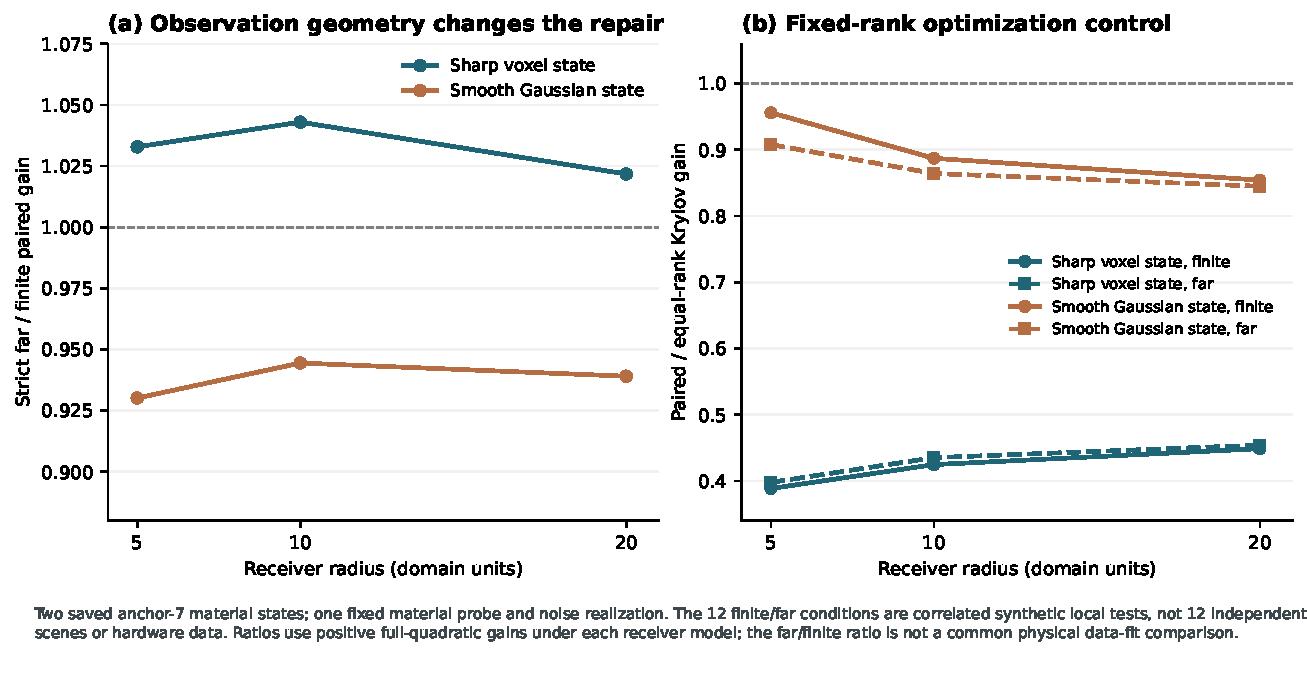
\includegraphics[width=0.96\textwidth]{figures/Figure_faemis_repair.pdf}
\caption{Receiver-dependent material-repair gains at two saved anchor-7 material states. (a) Strict-far paired gain divided by finite-receiver paired gain at the same radius. (b) Paired gain divided by equal-real-rank (48) material Krylov gain within each receiver and its own full local quadratic. The probe and absolute complex-noise realization are fixed per state; the residuals are synthetic. The 12 finite/far receiver/state conditions are correlated local tests, not independent scenes, hardware measurements, or reconstruction-error comparisons.}
\label{fig:faemis-repair}
\end{figure*}

\begin{figure}[tbp]\centering
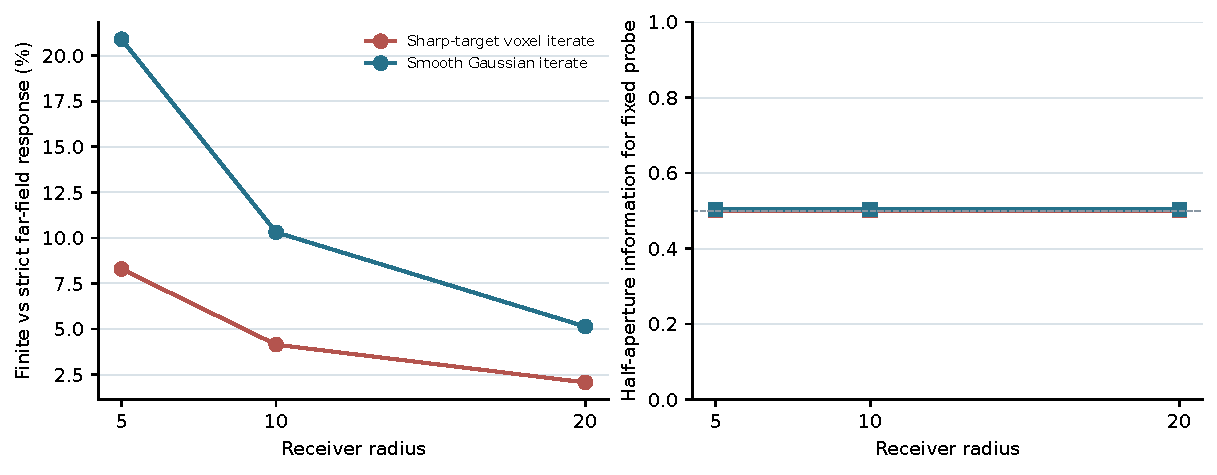
\includegraphics[width=0.98\columnwidth]{figures/Figure_farfield_aperture.pdf}
\caption{Synthetic receiver-design checks at two saved \(12^3\) material states. Radii 5, 10, and 20 use the same nondimensional length unit as the side-1.5 computational box and wavenumber 2.5. The strict far-field response is matched to each radius in propagation phase and \(1/r\) amplitude before taking a complex relative norm. Half-aperture information is one predeclared material-probe quadratic ratio, not a full-Jacobian singular-value or paired-repair bound.}
\end{figure}

\begin{figure}[tbp]\centering
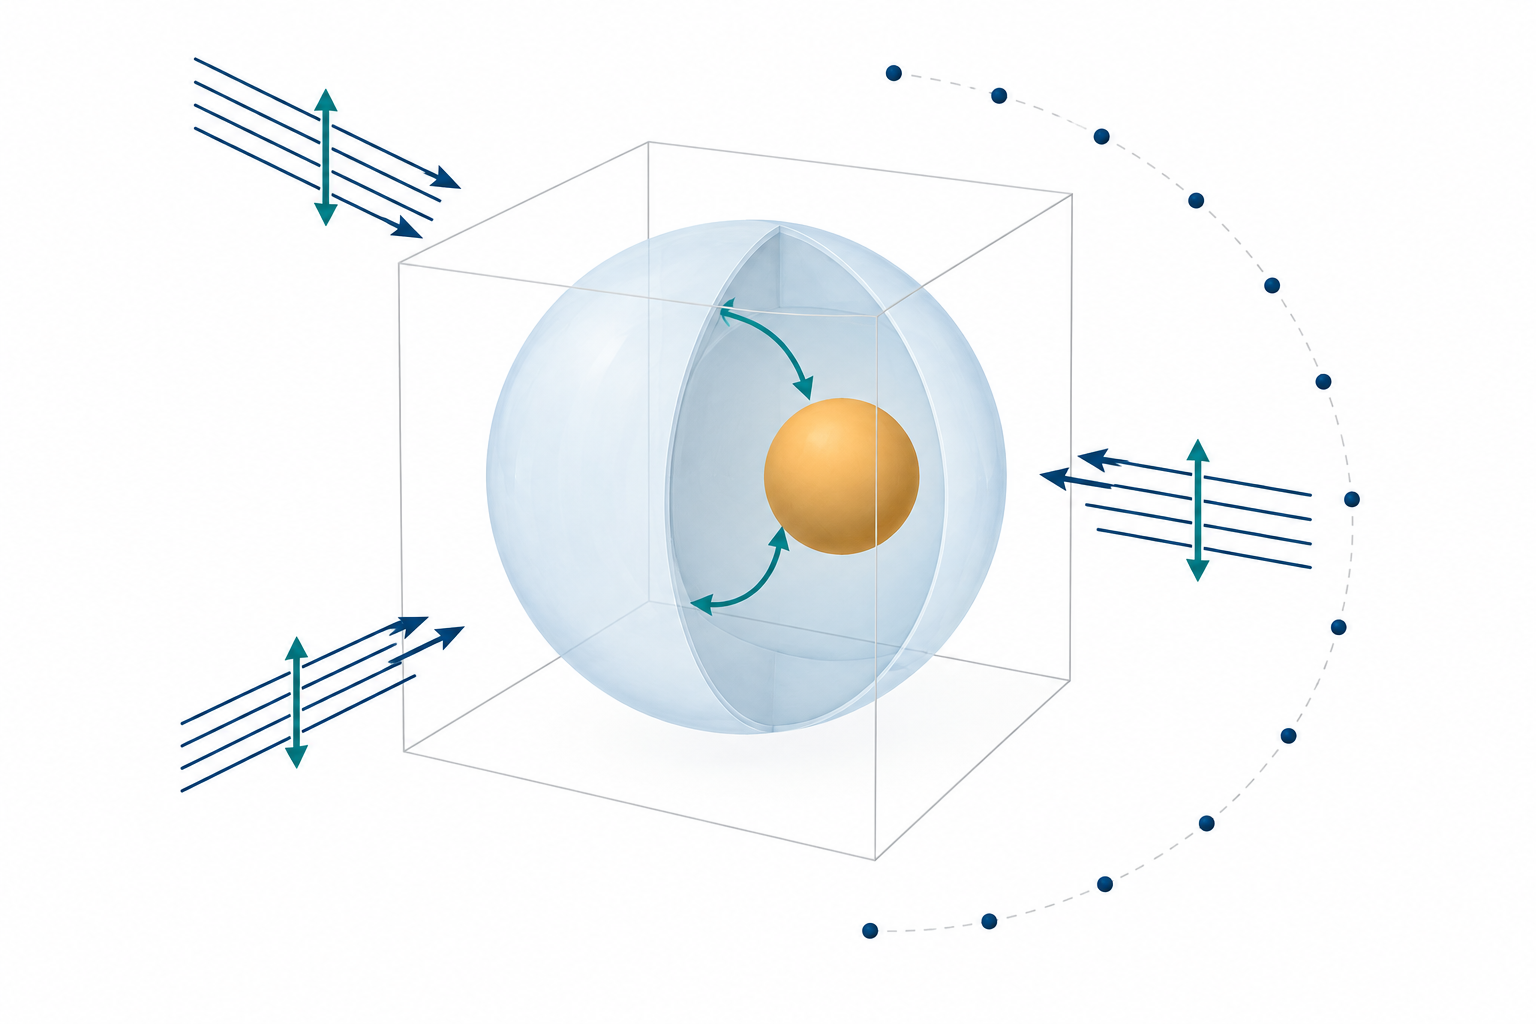
\includegraphics[width=0.96\columnwidth]{figures/scene_concept_3d.png}
\caption{Conceptual three-dimensional receiver scene: a sharply bounded dielectric object is illuminated from multiple directions, induces internal rescattering currents, and is observed in two transverse polarizations. The illustration describes acquisition geometry; it is not a computed field, reconstruction, or experimental datum.}
\end{figure}

\subsection*{Sharp-Interface Vector-Maxwell Challenge}

The preceding mechanism tests used smooth targets, which do not probe interface recovery. We therefore froze four higher-contrast geometries before running a new campaign: a homogeneous sphere, a two-material split rectangular solid, an eccentric-core shell, and two separated dielectric ellipsoids. All are in a vacuum box of side 1.5 at wavenumber 2.5, with six incident fields and dual-polarization reception. The new comparison uses physically normalized voxel material coordinates without giving the inverse solver true boundaries or regions. Truth is generated on a \(14^3\) grid and fitted on a \(12^3\) grid, within the same discrete-dipole family; same-grid \(14^3\) checks are labeled separately. The full-model preconditioned-CG route and a fixed \emph{Gs24 spectral selection rule} share initial material, regularization, constraints, noise realization, and nonlinear acceptance rule. The latter uses fresh primal anchors and state-dependent operators at each iteration, not a stale physical state or immutable current basis. Neither route executes the paired material repair. The sharp-scene record is reported separately from the original 72 correlated smooth-state local comparisons.

At \(12^3\), complex voxel contrast has 3456 real coordinates but the six illuminations provide only \(6\times128=768\) complex, or 1536 real, receiver values. The local material Jacobian is necessarily rank deficient before prior information. A small measurement residual cannot therefore certify a sharp material interface; recovery must be judged against the declared prior and truth as a separate endpoint.

We first quantify the full-wave/Born response difference, because large dielectric contrast alone does not prove a large retained-feedback contribution. Reconstruction assessment then uses real and imaginary material error on a common physical grid, fixed-threshold interface overlap, class-average contrast, held-out receiver data, true nonlinear objective reduction, fallback counts, and total cost. Local current-bank comparisons at full-model iterates 0, 3, and 7 use that iterate's actual damping. This distinction matters: the previous local bank study fixed a diagnostic curvature and cannot stand in for the new nonlinear-state comparisons.

All 16 frozen primary trajectories completed. Table~\ref{tab:sharp-primary} reports the zero-noise endpoints; the 1\% complex-noise cases use the same noise realization for both methods. The full-model route has smaller material and held-out-field errors in six of eight method pairs, but this relative ordering does not amount to successful sharp-interface inversion. Across the eight full-model runs, the median final/initial true-objective ratio is 0.00229, and the median fallback count is 12.5; objective decrease is therefore substantial despite weak material recovery. For example, the homogeneous sphere reaches 2.73\% held-out response error while its complex material error remains 75.52\% and thresholded support overlap is only 2.63\%. Its recovered mean interior real contrast is 1.91 versus the specified 5.0. The two separated ellipsoids are not recovered by either route: support overlap is zero in both noise conditions, and the true real-contrast-7 class averages only 0.78 in the zero-noise full-model image. The shell is the best-recovered case by support overlap, about 69.25\% for the zero-noise full-model run, although its complex material error remains 56.03\% and the contrast-7 core averages 3.73. These are endpoint measurements against the specified discrete truth, not estimates of continuum material error.

\begin{table}[tbp]\centering\caption{Frozen sharp-interface primary endpoints at zero measurement noise. Material error is the relative complex contrast error; IoU is thresholded outer-support overlap; held-out error uses receiver data omitted from fitting. The last column is the full-model response difference from its first-Born counterpart at the true discrete material. Every row compares a full-model preconditioned-CG update (F) with a fixed current-space update (R), each after at most 18 accepted nonlinear iterations. The two routes have different accuracy, so their run times are not a matched-quality acceleration comparison.}\label{tab:sharp-primary}
\resizebox{\columnwidth}{!}{\begin{tabular}{lrrrrrrr}\hline
Target & Mat. F & Mat. R & IoU F & IoU R & Held-out F & Held-out R & Full/Born \\\hline
Sphere & .755 & .766 & .026 & .000 & .027 & .032 & .695\\
Split cuboid & .750 & .757 & .455 & .437 & .047 & .055 & .606\\
Eccentric shell & .560 & .587 & .692 & .675 & .019 & .026 & .736\\
Two ellipsoids & .906 & .901 & .000 & .000 & .073 & .072 & .335\\\hline
\end{tabular}}
\end{table}

The full/Born differences range from 33.5\% to 73.6\%. The separated ellipsoids have the highest constituent contrast but the smallest measured departure from Born in this set. Material contrast alone is therefore a poor proxy for the realized multiple-scattering strength under a given geometry and illumination. The fixed current-space route is sometimes faster in wall time, but it does not reach the same material or data endpoint in the six pairs where the full route wins. We accordingly do not infer an inverse-solver speedup from these unequal-quality runs.

At the saved full-model pre-update states 0, 3, and 7 for each zero-noise target, we also compared three specified current banks (residual, Gs, and TSOM-inspired) under the \emph{same full regularized local quadratic}, using the actual damping of that update. These bank labels identify candidate generators, not complete native SOM or TSOM algorithms. Across 36 correlated scene--state--bank rows, the paired material repair improves the specified direct current enlargement in 36/36, while equal-real-rank material Krylov improves the paired repair in 36/36. Both material banks have rank 48 in every comparison. The paired-gain median is \(2.81\times10^{-4}\), between the direct-enlargement median \(1.79\times10^{-5}\) and Krylov median \(5.18\times10^{-4}\); two direct enlargements even increase the full quadratic. The prescribed step change lies in the computed paired envelope to a median relative \(H\)-distance \(1.12\times10^{-11}\) (maximum \(3.14\times10^{-10}\)). These are local, highly correlated comparisons and do not represent paired nonlinear reconstruction trajectories. Their agreement with the original 72-comparison ordering supports the mechanism beyond smooth targets while retaining the negative equal-rank result. Supplement S11 lists every row and the associated absolute distances.

The retained feedback has appreciable size in these sharp states: in 16/36 banks its radiated norm exceeds that of the direct candidate current, with a maximum feedback/direct ratio of 11.20. The total dressed/direct output ratio has median 1.25 and maximum 11.25. Thus inspecting only the raw radiation of a proposed current can miss a larger retained-space-mediated output. The ratio is not a material information score, and it does not determine the objective gain without the injection side and current full defect.

\begin{figure*}[tbp]\centering
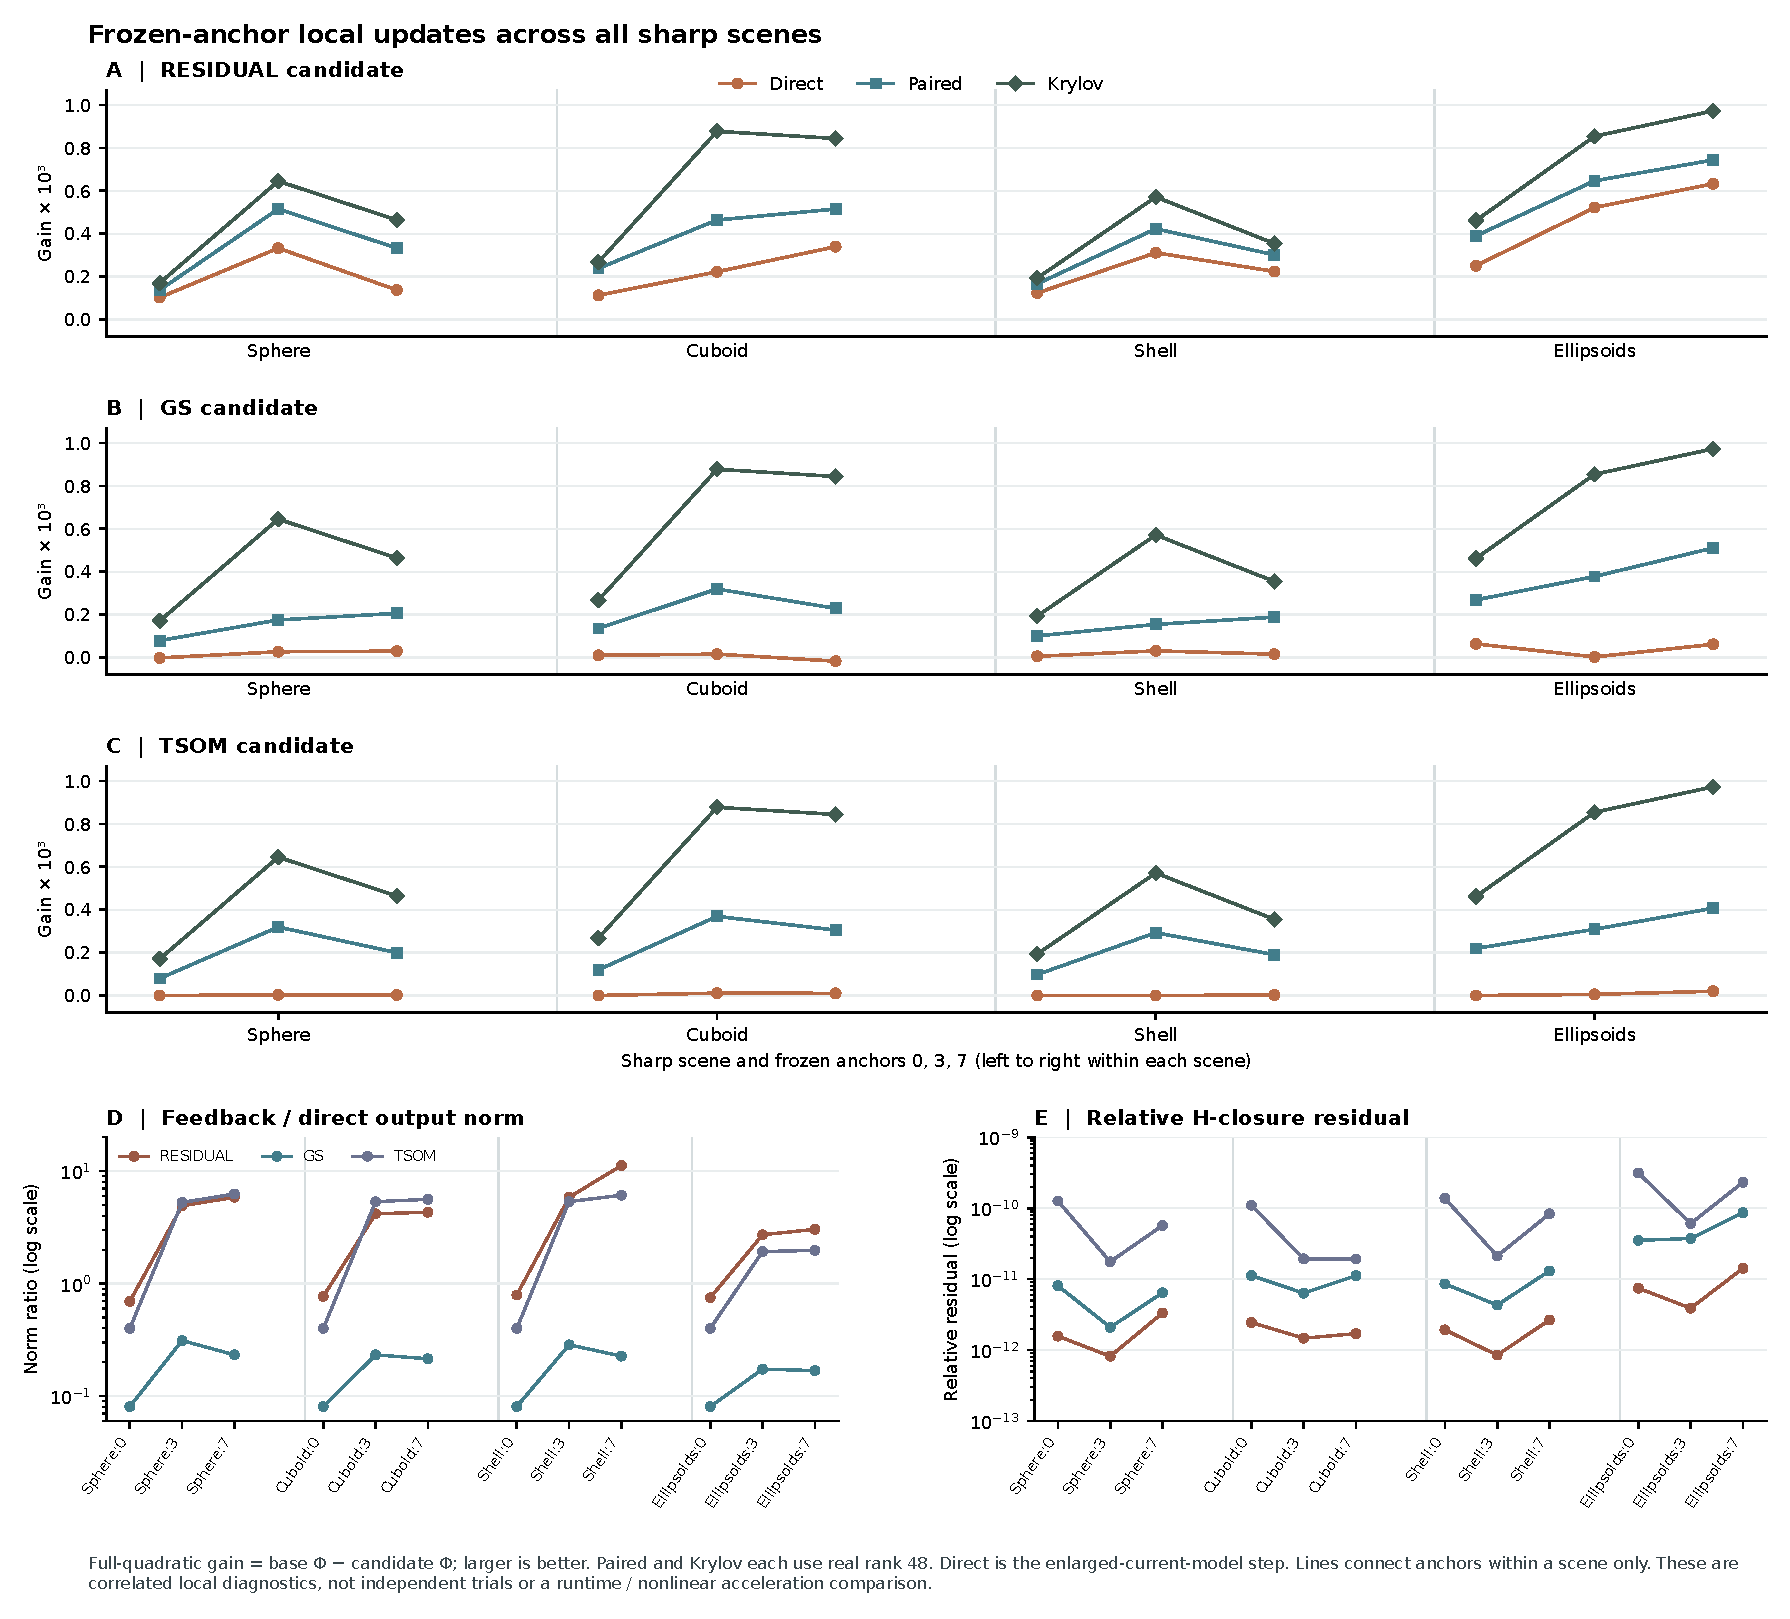
\includegraphics[width=0.96\textwidth]{figures/Figure_sharp_local.pdf}
\caption{Specified-bank local repair on four sharp vector-Maxwell targets. Three bank sources share each of 12 saved material states. The upper panels compare decrease in the same full regularized local quadratic for direct current enlargement, paired material repair, and equal-real-rank (48) material Krylov. The lower panels show retained-feedback/direct radiation and relative \(H\)-closure distance. All 36 rows are correlated frozen-state diagnostics rather than independent reconstructions; a negative direct gain is a worse full quadratic.}
\label{fig:sharp-local}
\end{figure*}

The predeclared 3\% noise extension covers only the split cuboid and eccentric shell, with a shared realization across the two methods. Full/fixed complex-material errors are 0.7501/0.7584 for the cuboid and 0.5830/0.5845 for the shell; corresponding held-out errors are 0.04666/0.05483 and 0.02454/0.02710. Material recovery remains limited, and the fixed shell route has slightly higher thresholded support overlap (0.6768 versus 0.6703). These four extension trajectories show that the primary negative material result is not confined to noiseless data, but do not establish general noise robustness.

The two predeclared same-grid \(14^3\) inverse-resolution pairs likewise do not resolve the material limitation. For the sphere, full/fixed complex-material errors are 0.7206/0.7366 and support overlaps are 0.0263/0; for the split cuboid, the corresponding values are 0.7153/0.7191 and 0.5980/0.5359. The cuboid boundary overlap improves relative to its \(12^3\) inversion, but its full-model held-out response error increases from 0.04655 to 0.05268. These same-family, same-grid runs are resolution checks, not independent continuum validation.

\begin{figure}[tbp]\centering
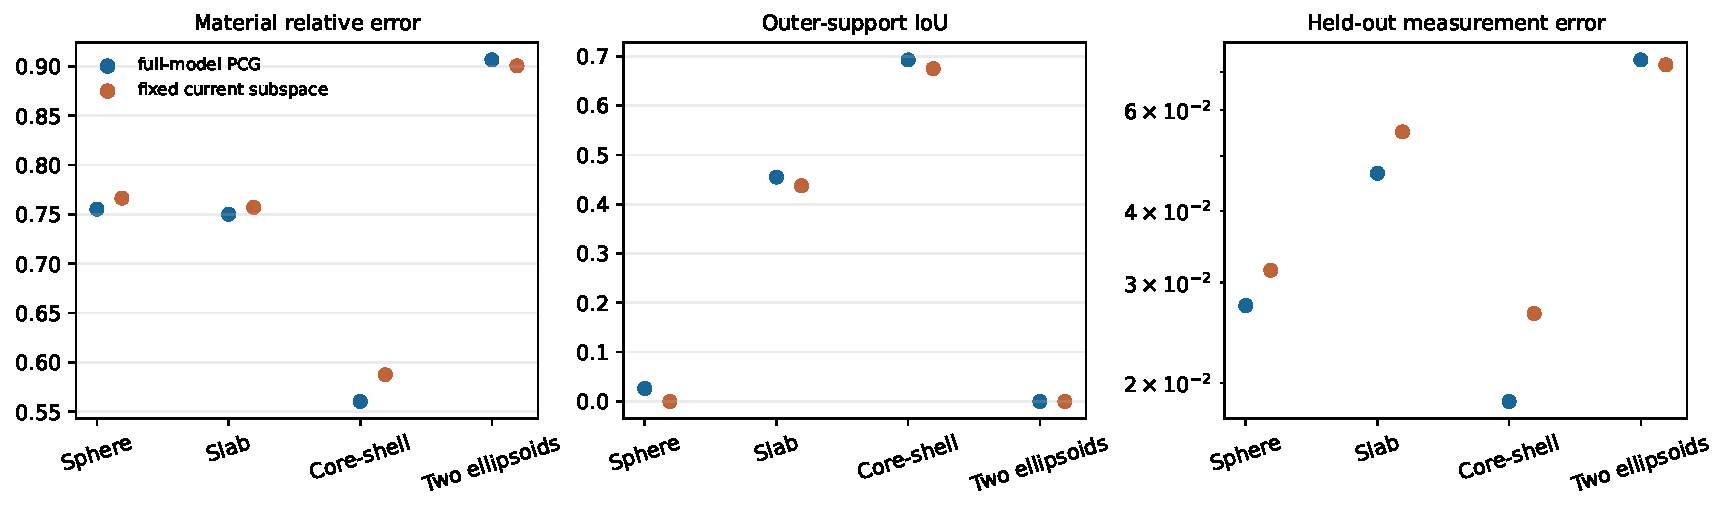
\includegraphics[width=0.98\columnwidth]{figures/Figure_sharp_primary_metrics.pdf}
\caption{Material error, held-out response error, and support overlap for the eight zero-noise trajectories in the 16-run primary campaign. Paired markers share the object, initialization, and acceptance rule. Small held-out response error can coexist with severe material and interface errors. The eight method pairs are correlated fixed scenarios, not a sample of 16 independent objects.}
\end{figure}

\begin{figure*}[tbp]\centering
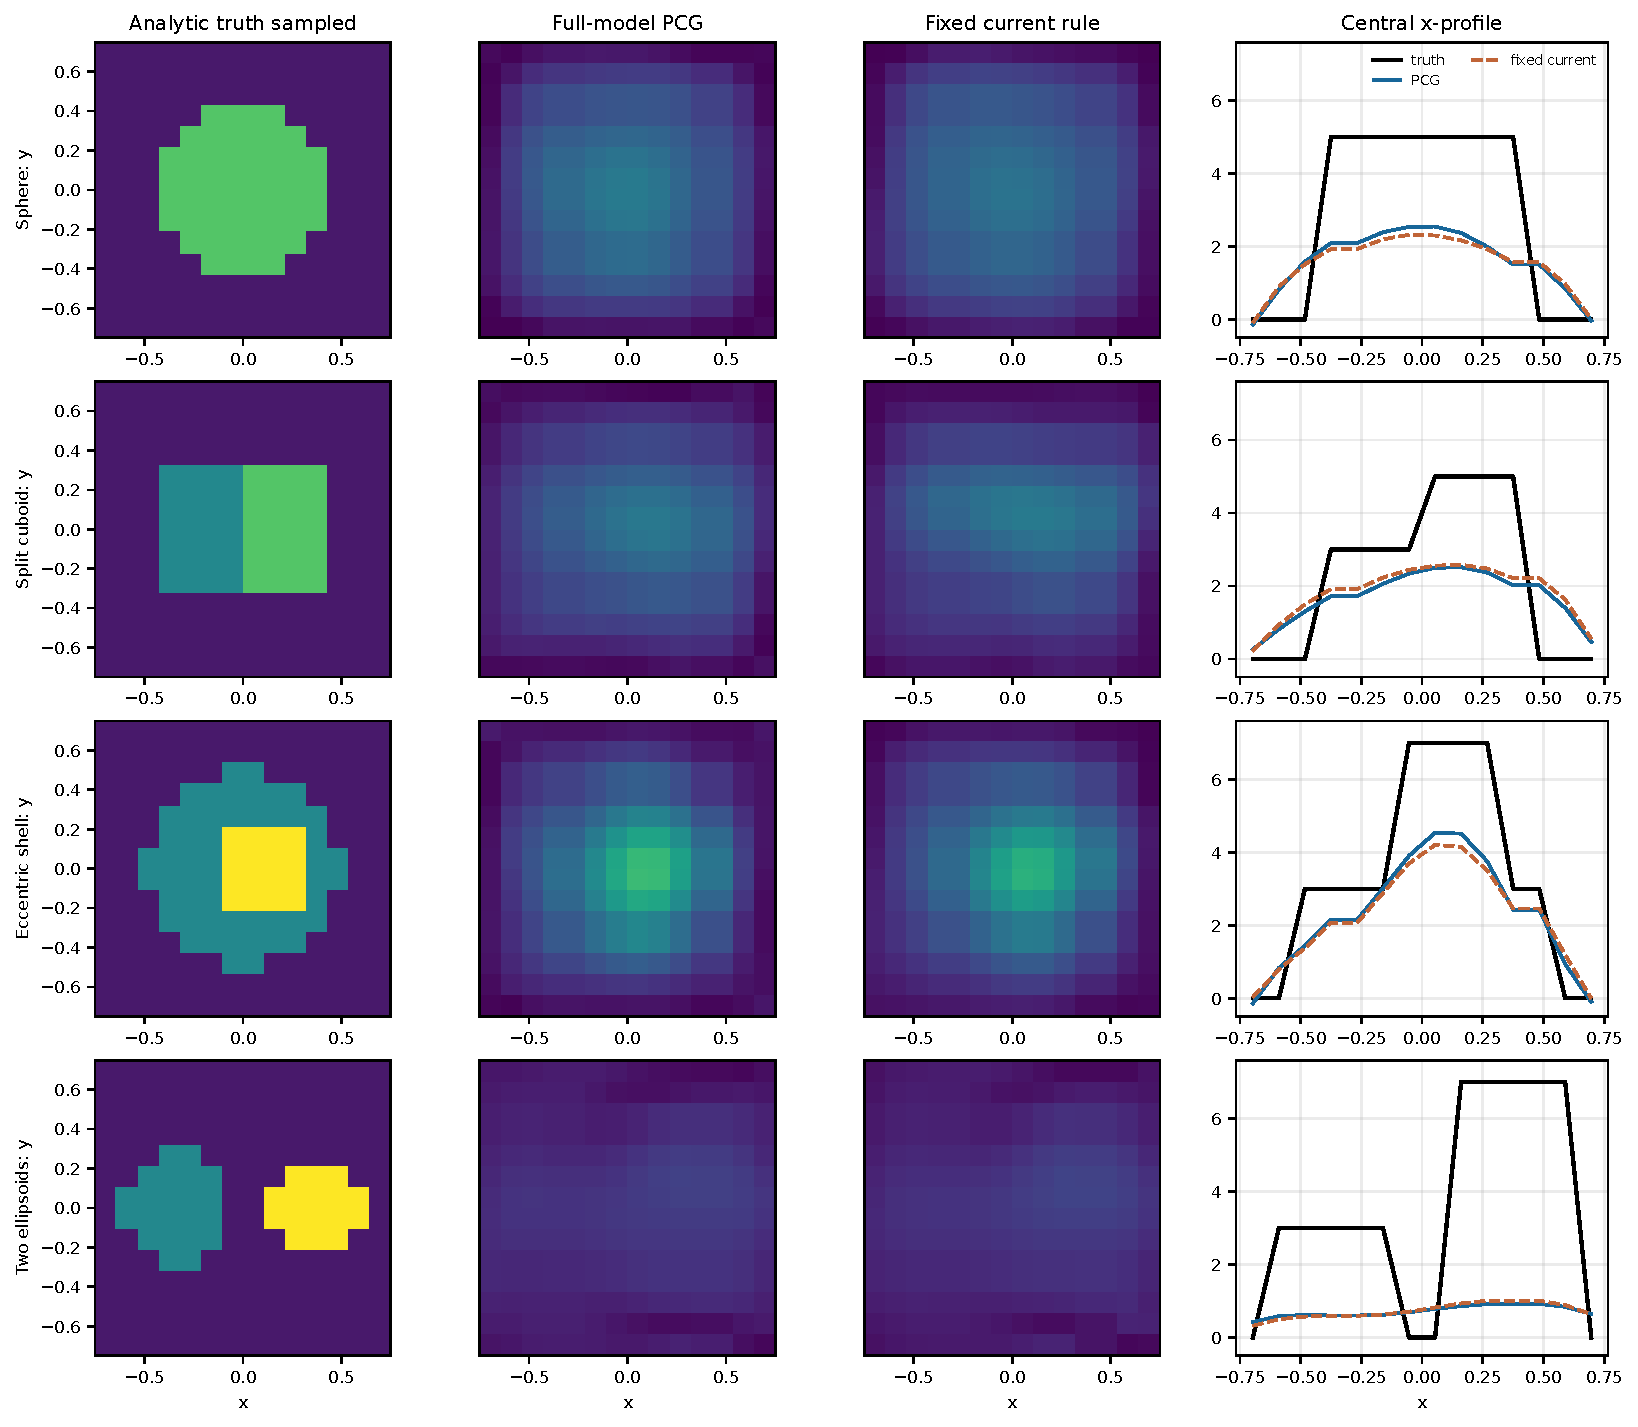
\includegraphics[width=0.96\textwidth]{figures/Figure_sharp_profiles.pdf}
\caption{Zero-noise real-contrast slices and central line profiles for all four frozen objects. The displayed truth is the analytic geometry sampled on the declared grid; reconstructions are mapped to that display grid with one common color scale. The full-model and fixed-current routes both smooth or miss sharp boundaries, particularly for the sphere and separated ellipsoids. This visualization supplements, rather than replaces, the complex-material and held-out-response metrics in Table~\ref{tab:sharp-primary}.}
\end{figure*}

An independent spherical-wave check places an important limit on the sharp-target validation. For the homogeneous sphere at contrast \(5+0.2i\), a predeclared forward receiver channel has complex-field relative errors of 21.40\% for the \(14^3\) DDA truth grid, 11.13\% at \(28^3\), and 9.73\% at \(32^3\), against the vector Mie series [15, main manuscript] after matching phase and far-field amplitude conventions. The finite voxel boundary makes convergence nonmonotone; this one-channel check is not a whole-aperture error bound. It nevertheless prevents interpreting the \(14^3\) same-family reference as a resolved continuum-Maxwell truth for this high-contrast sharp sphere. We keep material reconstruction and receiver-fit results relative to the declared discrete truth and do not transfer local ROM-step closure to continuum accuracy.

\begin{figure}[tbp]\centering
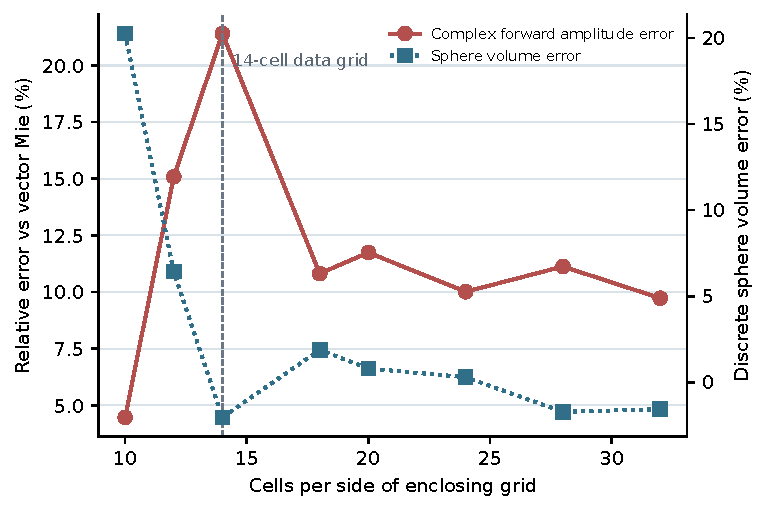
\includegraphics[width=0.98\columnwidth]{figures/Figure_mie_sharp_sphere.pdf}
\caption{Independent vector Mie comparison for one predeclared forward far-field channel of the high-contrast sphere. Complex-field errors are nonmonotone across voxel grids and remain 21.40\% at the \(14^3\) grid used to generate the main discrete truth. The plot is a forward-discretization diagnostic, not a bound for every receiver or a validation of recovered material.}
\end{figure}


\clearpage
\section*{S19. Frozen-state matched-history reuse protocol}
This experiment solves the complete material normal equation at saved states; it does not generate a new nonlinear reconstruction dataset. The common state includes the current factorization, material tangent, retained current basis, and baseline inverse. The prescribed residual sequence contains eight independent seeded complex Gaussian perturbations, each with norm 1\% of the fixed measured-data norm. The same perturbation is used by all methods. Middle-state histories come from the initial saved state; late-state histories come from the middle saved state.

To isolate preconditioning from initialization, every route receives a preceding converged full-normal step computed in a common preparation sequence. Preparation is timed separately. This paired-start contract is stronger than comparing each method from a different warm start, but it is not a deployable autonomous trajectory. Full experiment accounting includes this preparation; marginal-use accounting assumes the shared starts and paid histories exist. A separate history-acquisition surcharge shows what happens if the previous solve must be purchased for reuse. This surcharge is measured once with the common instrumented history collector, which saves both material directions and current snapshots; it is not a separately optimized cold-start collector for each method. The timed target-state plain baseline saves no unnecessary current snapshots.

The plain baseline never saves current snapshots during a timed solve. The current-derived inverse uses at most twelve columns obtained from the previous state's adjoint-current snapshots. Its construction is frozen for all eight right-hand sides. An eight-probe diagnostic is charged once, regardless of whether its sufficient condition passes. The initial six paid full-H actions supply history; they can include the initial-guess action and must not all be called search directions.

\begin{figure}[htbp]\centering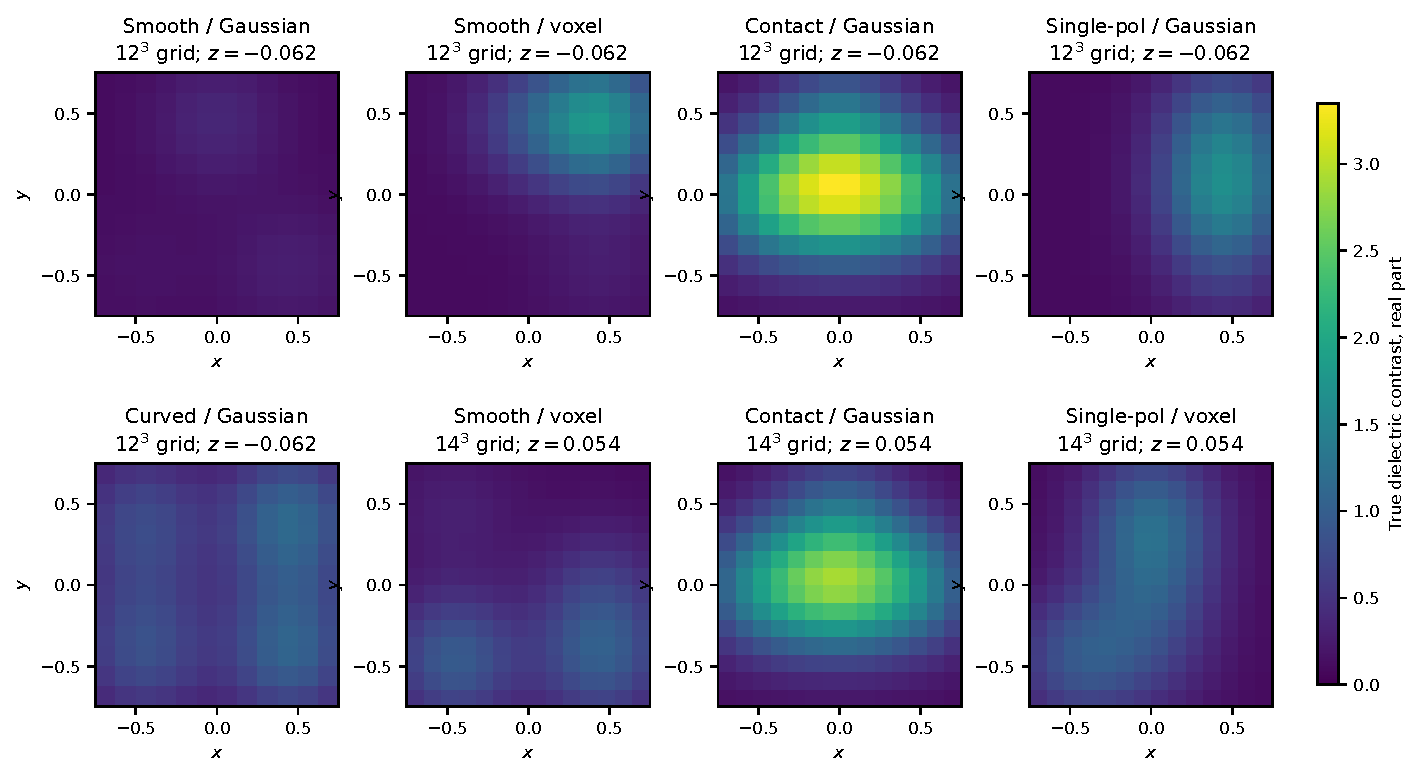
\includegraphics[width=\linewidth]{figures/frozen_objects.pdf}
\caption{Saved target slices for the eight smooth-object cases, using one common real-contrast color scale. These are target fields, not reconstructions. The nearest sampled central $z$ plane is reported for each grid. Gaussian/voxel labels refer to the material tangent used in inversion; ``Single-pol'' changes illumination polarization, not receiver aperture. These are distinct existing objects, so the panels are not a matched representation comparison.}
\end{figure}

\subsection*{State and history separation}
The eight smooth-object saved states use scalar regularization 0.00301 at index 3 and 0.00091 at index 7. Their current banks come from indices 0 and 3, respectively. In the volume-weighted material norm, the relative change from the historical material to the target material ranges from 0.963 to 7.911 for the former pair and from 0.0346 to 0.1512 for the latter. Consequently, an intermediate/late performance difference changes both damping and the proximity of the available history; it does not isolate either as its cause. The two sharp stress states use the same late-state regularization, with relative historical-material changes 0.317 and 0.192. These are extracted state descriptors, not new forward solves or input to the frozen selection rule; the full values are in \texttt{ANCHOR\_STATE\_METADATA.csv}.

\subsection*{Standard material-space two-level comparison}
Let $Z$ contain retained real material directions and $E=Z^THZ$. Define
\[
P=I-ZE^{-1}Z^TH,\qquad
M_{\mathrm{two}}=ZE^{-1}Z^T+PM_0P^T.
\]
For a positive-definite $H,M_0$ and independent $Z$, this inverse action is symmetric positive definite and $M_{\mathrm{two}}HZ=Z$. The implementation applies the two coarse projections and the base inverse without forming $P$. The coarse space is constant throughout a PCG solve. Only after that solve does the method append its own newly paid material directions and reselect generalized Ritz directions using the projected pair $(Z^THZ,Z^TH_0Z)$.

This is a balanced two-level/deflated preconditioner. The general augmentation/deflation framework explains its connection to projected Krylov correction; the code is not claimed to reproduce every singular projected solver in that literature. A separate recent-six coarse warm-start control applies a correction only to the starting vector and is labeled accordingly.

The storage budget equals the current method's extra persistent numerical arrays, excluding references to the common state and baseline inverse. The material method stores $Z,HZ,E$ and its Cholesky factor; the cached sensitivity also includes retained Ritz values. Actual ranks are recorded because a complex current column and a real material column have different dimensions and costs. On a 54-dimensional Gaussian material tangent, this byte budget can eventually admit all 54 directions. Such a full-rank projected spectrum is learned from paid actions, not supplied by an offline oracle. Temporary history and factorization memory are recorded separately from persistent storage.

\subsection*{Finite precision and the cached-image sensitivity}
For nearly dependent columns, forming $HZV\Sigma^{-1}$ can amplify roundoff. A robust realization recomputes $H$ on the rank-revealed basis; all these actions and the associated wall time are charged. Local tests on SPD, clustered, exactly rank-deficient, and nearly dependent histories give coarse-exactness errors below $2.1\times10^{-13}$ across relative dependency scales from $10^{-4}$ to $10^{-14}$.

The separately named cached-image sensitivity uses a stronger normalized singular-value cutoff of $10^{-6}$. Historical images from a different state are refreshed once. Same-state reselection reuses already paid $HZ$, with up to four deterministic orthonormal span checks. An image discrepancy exceeding $10^{-9}\lambda$ times the checked direction norm triggers a paid complete retained-basis refresh. The check is a numerical consistency guard, not a certificate over untested directions. No diagonal jitter is inserted to hide an indefinite coarse matrix.

The cached implementation is reported separately because it changes the numerical realization and the rank cutoff. Its rule was fixed using development evidence before examining validation outcomes. The robust implementation remains in the raw record. A timing lower bound that removes maintenance is explicitly an optimistic sensitivity, not an implemented method.

\subsection*{What the charged Gaussian check certifies}
The repeated-solve experiment checks a normalized Hessian difference, rather than directly estimating the Jacobian-tail quantity $\eta_U$. With $M_C=FF^T$, let $A=F^T(H-H_C)F$. Eight independently generated standard real Gaussian vectors give
\[
\widehat\epsilon_H=2\max_{1\le j\le8}\|Ag_j\|.
\]
For a fixed candidate independent of these probes, the probability that $\widehat\epsilon_H<\|A\|_2$ is at most $\Pr(|N(0,1)|<1/2)^8\simeq4.62\times10^{-4}$. If the bound is below1, the symmetric preconditioned spectrum lies in $[1-\widehat\epsilon_H,1+\widehat\epsilon_H]$ with that probability guarantee. An acceptance flag uses the stricter threshold0.6. Performance measurements still run the SPD inverse when the flag rejects, so they are empirical tests rather than a certified deployment policy.

The five timing repetitions reuse the same fixed probes and candidate, and are not five independent probability events. Across18 distinct tested frozen states, a union bound is at most0.00833; it is conservative and does not claim probe completeness. Construction of the inverse square-root factors and all eight full-H actions are charged. The full-Hessian check and the earlier regularization-whitened Jacobian bounds are separate quantities in the evidence record.

\subsection*{Stopping, timing, and units of evidence}
All timed routes use FP64, the same full $H,h$, regularization, and relative true normal residual threshold $10^{-8}$. PCG has at most 150 steps and checks the actual residual, with replacement if a recursive residual is misleading. Every row records achieved residual, full-wave right-hand sides, setup, application, capture, reselection, and total time. Small-system spectra and exact full spectra used for interpretation are excluded from online selection and separately charged.

Five repetitions use identical physical data and rotate method order. Their median and interquartile range quantify timing variability. Eight noise residuals are eight uses of one state, not independent objects. Middle and late states of one object are also correlated. Overall validation summaries aggregate at object level. Development objects, six rule-validation objects, and two sharp stress objects remain distinct groups.

A sustained break-even use is the first use after which cumulative current-method cost remains below matched baseline cost through the eighth use. It includes construction and the diagnostic check. An absent break-even is recorded, not extrapolated from average iteration savings. If history is not already available, its measured acquisition cost is added as a separate surcharge. Initial geometry/operator assembly and experiment bookkeeping are also contained in the complete monitored job time, but are not isolated as separately repeated per-method phases. Accordingly, route comparisons are labeled marginal or paired-common-cost comparisons; the occupation ledger gives the total campaign expenditure, not an autonomous cold-start speedup.

\noindent Ratios compare eight complete solves with the same-phase baseline. Cost cells give median [Q1,Q3] over five timing repetitions. Paid history adds the previous-state instrumented history acquisition. All quality outcomes are retained.
\par Rank labels: C/W are complex current/signature ranks; R is the real material coarse rank. They are different spaces. Diagnostic counts and KiB are medians; the machine-readable record retains every repetition. Sustained break-even (BE) is the number of successful repetitions followed by the minimum--maximum use index.
\par\medskip\noindent\begin{minipage}{\linewidth}\textbf{Development --- Paid-refresh Ritz (part 1)}
\begin{center}\fontsize{8}{10}\selectfont\setlength{\tabcolsep}{3pt}
\resizebox{\textwidth}{!}{\begin{tabular}{llccc}
\toprule Case/state & Method & Available history ratio & History charged ratio & History (s)\\\midrule
Smooth G12 / mid & Current & 0.998 [0.995,1.004] & 1.420 [1.418,1.431] & 4.49\\
Smooth G12 / mid & Ritz & 3.676 [3.651,3.684] & 4.098 [4.072,4.111] & 4.49\\
Smooth G12 / mid & Warm start & 1.153 [1.141,1.159] & 1.575 [1.561,1.585] & 4.49\\
Smooth G12 / late & Current & 0.802 [0.802,0.805] & 1.197 [1.196,1.203] & 5.32\\
Smooth G12 / late & Ritz & 2.851 [2.836,2.872] & 3.248 [3.232,3.266] & 5.32\\
Smooth G12 / late & Warm start & 1.110 [1.109,1.110] & 1.506 [1.504,1.506] & 5.32\\
Smooth V12 / mid & Current & 1.000 [0.998,1.004] & 1.278 [1.272,1.281] & 4.88\\
Smooth V12 / mid & Ritz & 3.633 [3.625,3.634] & 3.911 [3.900,3.912] & 4.88\\
Smooth V12 / mid & Warm start & 1.082 [1.077,1.086] & 1.357 [1.351,1.363] & 4.88\\
Smooth V12 / late & Current & 0.733 [0.731,0.738] & 0.989 [0.982,0.996] & 6.07\\
Smooth V12 / late & Ritz & 3.374 [3.356,3.382] & 3.630 [3.610,3.638] & 6.07\\
Smooth V12 / late & Warm start & 1.052 [1.046,1.054] & 1.307 [1.300,1.310] & 6.07\\
\bottomrule\end{tabular}}\end{center}
\end{minipage}
\begin{center}\fontsize{8}{10}\selectfont\setlength{\tabcolsep}{3pt}
\resizebox{\textwidth}{!}{\begin{tabular}{llccccc}
\toprule Case/state & Method & Rank & KiB & Full-wave RHS & True residual & Sustained BE\\\midrule
Smooth G12 / mid & Current & C12/W27 & 1445.8 & 1128 & 8.57e-09 & 3/5: 8--8\\
Smooth G12 / mid & Ritz & R4--54 & 91.1 & 5406 & 7.78e-09 & none (0/5)\\
Smooth G12 / mid & Warm start & R4--6 & 5.3 & 1320 & 6.47e-09 & none (0/5)\\
Smooth G12 / late & Current & C12/W27 & 1445.8 & 1152 & 2.63e-09 & 5/5: 3--3\\
Smooth G12 / late & Ritz & R6--54 & 91.1 & 5286 & 8.98e-09 & none (0/5)\\
Smooth G12 / late & Warm start & R6--6 & 5.3 & 1608 & 7.22e-09 & none (0/5)\\
Smooth V12 / mid & Current & C12/W144 & 16226.6 & 1632 & 8.74e-09 & 3/5: 8--8\\
Smooth V12 / mid & Ritz & R6--88 & 4873.0 & 8796 & 6.76e-09 & none (0/5)\\
Smooth V12 / mid & Warm start & R6--6 & 324.3 & 1992 & 7.88e-09 & none (0/5)\\
Smooth V12 / late & Current & C12/W144 & 16226.6 & 1620 & 7.22e-09 & 5/5: 2--3\\
Smooth V12 / late & Ritz & R6--110 & 6129.1 & 11016 & 7.24e-09 & none (0/5)\\
Smooth V12 / late & Warm start & R6--6 & 324.3 & 2604 & 9.29e-09 & none (0/5)\\
\bottomrule\end{tabular}}\end{center}
\par\medskip\noindent\begin{minipage}{\linewidth}\textbf{Development --- Cached-image Ritz (part 1)}
\begin{center}\fontsize{8}{10}\selectfont\setlength{\tabcolsep}{3pt}
\resizebox{\textwidth}{!}{\begin{tabular}{llccc}
\toprule Case/state & Method & Available history ratio & History charged ratio & History (s)\\\midrule
Smooth G12 / mid & Current & 0.998 [0.996,0.999] & 1.430 [1.430,1.432] & 4.77\\
Smooth G12 / mid & Ritz & 1.122 [1.122,1.124] & 1.555 [1.554,1.556] & 4.77\\
Smooth G12 / late & Current & 0.808 [0.807,0.809] & 1.203 [1.202,1.205] & 5.50\\
Smooth G12 / late & Ritz & 0.918 [0.917,0.919] & 1.311 [1.310,1.316] & 5.50\\
Smooth V12 / mid & Current & 1.012 [1.011,1.015] & 1.292 [1.290,1.293] & 5.08\\
Smooth V12 / mid & Ritz & 0.986 [0.984,0.986] & 1.264 [1.263,1.264] & 5.08\\
Smooth V12 / late & Current & 0.740 [0.740,0.741] & 0.997 [0.996,0.998] & 6.35\\
Smooth V12 / late & Ritz & 0.858 [0.855,0.859] & 1.115 [1.111,1.115] & 6.35\\
\bottomrule\end{tabular}}\end{center}
\end{minipage}
\begin{center}\fontsize{8}{10}\selectfont\setlength{\tabcolsep}{3pt}
\resizebox{\textwidth}{!}{\begin{tabular}{llccccc}
\toprule Case/state & Method & Rank & KiB & Full-wave RHS & True residual & Sustained BE\\\midrule
Smooth G12 / mid & Current & C12/W27 & 1445.8 & 1128 & 8.57e-09 & 5/5: 8--8\\
Smooth G12 / mid & Ritz & R4--50 & 81.6 & 1440 & 7.78e-09 & none (0/5)\\
Smooth G12 / late & Current & C12/W27 & 1445.8 & 1152 & 2.63e-09 & 5/5: 3--3\\
Smooth G12 / late & Ritz & R6--54 & 91.5 & 1488 & 8.98e-09 & 5/5: 8--8\\
Smooth V12 / mid & Current & C12/W144 & 16226.6 & 1632 & 8.74e-09 & none (0/5)\\
Smooth V12 / mid & Ritz & R6--83 & 4590.3 & 1896 & 7.51e-09 & 5/5: 8--8\\
Smooth V12 / late & Current & C12/W144 & 16226.6 & 1620 & 7.22e-09 & 5/5: 3--3\\
Smooth V12 / late & Ritz & R6--106 & 5900.4 & 2196 & 9.00e-09 & 5/5: 5--5\\
\bottomrule\end{tabular}}\end{center}
\par\medskip\noindent\begin{minipage}{\linewidth}\textbf{Validation --- Paid-refresh Ritz (part 1)}
\begin{center}\fontsize{8}{10}\selectfont\setlength{\tabcolsep}{3pt}
\resizebox{\textwidth}{!}{\begin{tabular}{llccc}
\toprule Case/state & Method & Available history ratio & History charged ratio & History (s)\\\midrule
Contact G12 / mid & Current & 0.951 [0.945,0.955] & 1.291 [1.285,1.299] & 4.82\\
Contact G12 / mid & Ritz & 2.255 [2.246,2.258] & 2.595 [2.587,2.601] & 4.82\\
Contact G12 / mid & Warm start & 1.111 [1.106,1.119] & 1.452 [1.446,1.462] & 4.82\\
Contact G12 / late & Current & 0.684 [0.679,0.691] & 0.993 [0.991,1.003] & 5.54\\
Contact G12 / late & Ritz & 1.669 [1.651,1.670] & 1.981 [1.959,1.983] & 5.54\\
Contact G12 / late & Warm start & 1.087 [1.084,1.091] & 1.397 [1.392,1.402] & 5.54\\
Single-pol G12 / mid & Current & 0.909 [0.895,0.911] & 1.249 [1.235,1.254] & 4.86\\
Single-pol G12 / mid & Ritz & 2.765 [2.748,2.768] & 3.107 [3.085,3.108] & 4.86\\
Single-pol G12 / mid & Warm start & 1.112 [1.104,1.115] & 1.452 [1.447,1.453] & 4.86\\
Single-pol G12 / late & Current & 0.716 [0.714,0.716] & 1.079 [1.078,1.080] & 5.59\\
Single-pol G12 / late & Ritz & 2.613 [2.613,2.614] & 2.976 [2.976,2.978] & 5.59\\
Single-pol G12 / late & Warm start & 1.086 [1.083,1.091] & 1.451 [1.449,1.454] & 5.59\\
\bottomrule\end{tabular}}\end{center}
\end{minipage}
\begin{center}\fontsize{8}{10}\selectfont\setlength{\tabcolsep}{3pt}
\resizebox{\textwidth}{!}{\begin{tabular}{llccccc}
\toprule Case/state & Method & Rank & KiB & Full-wave RHS & True residual & Sustained BE\\\midrule
Contact G12 / mid & Current & C12/W27 & 1445.8 & 1428 & 6.99e-09 & 5/5: 5--6\\
Contact G12 / mid & Ritz & R6--54 & 91.1 & 4350 & 7.90e-09 & none (0/5)\\
Contact G12 / mid & Warm start & R6--6 & 5.3 & 1692 & 7.05e-09 & none (0/5)\\
Contact G12 / late & Current & C12/W27 & 1445.8 & 1296 & 9.72e-09 & 5/5: 2--2\\
Contact G12 / late & Ritz & R6--54 & 91.1 & 4020 & 3.97e-09 & none (0/5)\\
Contact G12 / late & Warm start & R6--6 & 5.3 & 2088 & 8.70e-09 & none (0/5)\\
Single-pol G12 / mid & Current & C12/W27 & 1445.8 & 1368 & 8.32e-09 & 5/5: 4--4\\
Single-pol G12 / mid & Ritz & R6--54 & 91.1 & 5424 & 3.82e-09 & none (0/5)\\
Single-pol G12 / mid & Warm start & R6--6 & 5.3 & 1704 & 3.31e-09 & none (0/5)\\
Single-pol G12 / late & Current & C12/W27 & 1445.8 & 1152 & 8.67e-09 & 5/5: 2--2\\
Single-pol G12 / late & Ritz & R6--54 & 91.1 & 5508 & 9.83e-09 & none (0/5)\\
Single-pol G12 / late & Warm start & R6--6 & 5.3 & 1788 & 9.76e-09 & none (0/5)\\
\bottomrule\end{tabular}}\end{center}
\par\medskip\noindent\begin{minipage}{\linewidth}\textbf{Validation --- Paid-refresh Ritz (part 2)}
\begin{center}\fontsize{8}{10}\selectfont\setlength{\tabcolsep}{3pt}
\resizebox{\textwidth}{!}{\begin{tabular}{llccc}
\toprule Case/state & Method & Available history ratio & History charged ratio & History (s)\\\midrule
Curved G12 / mid & Current & 0.835 [0.834,0.838] & 1.168 [1.167,1.169] & 4.88\\
Curved G12 / mid & Ritz & 2.259 [2.258,2.261] & 2.592 [2.591,2.592] & 4.88\\
Curved G12 / mid & Warm start & 1.111 [1.109,1.111] & 1.442 [1.439,1.443] & 4.88\\
Curved G12 / late & Current & 0.710 [0.704,0.714] & 1.029 [1.023,1.031] & 5.33\\
Curved G12 / late & Ritz & 2.119 [2.065,2.119] & 2.438 [2.378,2.442] & 5.33\\
Curved G12 / late & Warm start & 1.095 [1.062,1.095] & 1.413 [1.377,1.418] & 5.33\\
Smooth V14 / mid & Current & 0.944 [0.943,0.949] & 1.326 [1.326,1.330] & 13.45\\
Smooth V14 / mid & Ritz & 3.605 [3.605,3.611] & 3.987 [3.985,3.993] & 13.45\\
Smooth V14 / mid & Warm start & 1.080 [1.079,1.082] & 1.462 [1.461,1.463] & 13.45\\
Smooth V14 / late & Current & 0.720 [0.719,0.720] & 1.058 [1.057,1.059] & 15.67\\
Smooth V14 / late & Ritz & 3.445 [3.443,3.450] & 3.783 [3.782,3.788] & 15.67\\
Smooth V14 / late & Warm start & 1.047 [1.047,1.048] & 1.386 [1.386,1.386] & 15.67\\
\bottomrule\end{tabular}}\end{center}
\end{minipage}
\begin{center}\fontsize{8}{10}\selectfont\setlength{\tabcolsep}{3pt}
\resizebox{\textwidth}{!}{\begin{tabular}{llccccc}
\toprule Case/state & Method & Rank & KiB & Full-wave RHS & True residual & Sustained BE\\\midrule
Curved G12 / mid & Current & C12/W27 & 1445.8 & 1260 & 8.22e-09 & 5/5: 3--3\\
Curved G12 / mid & Ritz & R5--54 & 91.1 & 4374 & 9.16e-09 & none (0/5)\\
Curved G12 / mid & Warm start & R5--6 & 5.3 & 1704 & 2.46e-09 & none (0/5)\\
Curved G12 / late & Current & C12/W27 & 1445.8 & 1212 & 8.42e-09 & 5/5: 2--2\\
Curved G12 / late & Ritz & R6--54 & 91.1 & 4674 & 9.95e-09 & none (0/5)\\
Curved G12 / late & Warm start & R6--6 & 5.3 & 1896 & 5.23e-09 & none (0/5)\\
Smooth V14 / mid & Current & C12/W144 & 25370.6 & 1728 & 4.80e-09 & 5/5: 6--6\\
Smooth V14 / mid & Ritz & R6--96 & 8376.0 & 9504 & 7.47e-09 & none (0/5)\\
Smooth V14 / mid & Warm start & R6--6 & 514.8 & 2196 & 7.17e-09 & none (0/5)\\
Smooth V14 / late & Current & C12/W144 & 25370.6 & 1728 & 7.02e-09 & 5/5: 2--2\\
Smooth V14 / late & Ritz & R6--119 & 10425.5 & 11934 & 8.98e-09 & none (0/5)\\
Smooth V14 / late & Warm start & R6--6 & 514.8 & 2796 & 9.79e-09 & none (0/5)\\
\bottomrule\end{tabular}}\end{center}
\par\medskip\noindent\begin{minipage}{\linewidth}\textbf{Validation --- Paid-refresh Ritz (part 3)}
\begin{center}\fontsize{8}{10}\selectfont\setlength{\tabcolsep}{3pt}
\resizebox{\textwidth}{!}{\begin{tabular}{llccc}
\toprule Case/state & Method & Available history ratio & History charged ratio & History (s)\\\midrule
Contact G14 / mid & Current & 0.923 [0.922,0.925] & 1.382 [1.382,1.386] & 12.93\\
Contact G14 / mid & Ritz & 2.218 [2.215,2.219] & 2.678 [2.674,2.680] & 12.93\\
Contact G14 / mid & Warm start & 1.086 [1.086,1.086] & 1.546 [1.546,1.546] & 12.93\\
Contact G14 / late & Current & 0.658 [0.656,0.658] & 1.084 [1.082,1.086] & 14.64\\
Contact G14 / late & Ritz & 1.613 [1.611,1.614] & 2.040 [2.037,2.041] & 14.64\\
Contact G14 / late & Warm start & 1.066 [1.064,1.067] & 1.493 [1.490,1.494] & 14.64\\
Single-pol V14 / mid & Current & 1.096 [1.091,1.098] & 1.480 [1.474,1.481] & 12.97\\
Single-pol V14 / mid & Ritz & 3.954 [3.951,3.959] & 4.338 [4.336,4.342] & 12.97\\
Single-pol V14 / mid & Warm start & 1.072 [1.072,1.074] & 1.457 [1.456,1.458] & 12.97\\
Single-pol V14 / late & Current & 0.719 [0.719,0.721] & 1.050 [1.049,1.053] & 15.47\\
Single-pol V14 / late & Ritz & 3.755 [3.755,3.757] & 4.087 [4.086,4.088] & 15.47\\
Single-pol V14 / late & Warm start & 1.039 [1.039,1.040] & 1.371 [1.370,1.371] & 15.47\\
\bottomrule\end{tabular}}\end{center}
\end{minipage}
\begin{center}\fontsize{8}{10}\selectfont\setlength{\tabcolsep}{3pt}
\resizebox{\textwidth}{!}{\begin{tabular}{llccccc}
\toprule Case/state & Method & Rank & KiB & Full-wave RHS & True residual & Sustained BE\\\midrule
Contact G14 / mid & Current & C12/W27 & 2017.3 & 1512 & 8.46e-09 & 5/5: 5--5\\
Contact G14 / mid & Ritz & R6--54 & 91.1 & 4608 & 7.64e-09 & none (0/5)\\
Contact G14 / mid & Warm start & R6--6 & 5.3 & 1800 & 7.14e-09 & none (0/5)\\
Contact G14 / late & Current & C12/W27 & 2017.3 & 1308 & 7.89e-09 & 5/5: 2--2\\
Contact G14 / late & Ritz & R6--54 & 91.1 & 4038 & 4.69e-09 & none (0/5)\\
Contact G14 / late & Warm start & R6--6 & 5.3 & 2148 & 9.28e-09 & none (0/5)\\
Single-pol V14 / mid & Current & C12/W144 & 25370.6 & 1920 & 5.43e-09 & none (0/5)\\
Single-pol V14 / mid & Ritz & R6--104 & 9087.0 & 9948 & 9.78e-09 & none (0/5)\\
Single-pol V14 / mid & Warm start & R6--6 & 514.8 & 2088 & 7.79e-09 & none (0/5)\\
Single-pol V14 / late & Current & C12/W144 & 25370.6 & 1740 & 9.49e-09 & 5/5: 2--2\\
Single-pol V14 / late & Ritz & R6--134 & 11771.1 & 13086 & 8.41e-09 & none (0/5)\\
Single-pol V14 / late & Warm start & R6--6 & 514.8 & 2796 & 9.48e-09 & none (0/5)\\
\bottomrule\end{tabular}}\end{center}
\par\medskip\noindent\begin{minipage}{\linewidth}\textbf{Validation --- Cached-image Ritz (part 1)}
\begin{center}\fontsize{8}{10}\selectfont\setlength{\tabcolsep}{3pt}
\resizebox{\textwidth}{!}{\begin{tabular}{llccc}
\toprule Case/state & Method & Available history ratio & History charged ratio & History (s)\\\midrule
Contact G12 / mid & Current & 0.950 [0.948,0.952] & 1.293 [1.288,1.294] & 5.01\\
Contact G12 / mid & Ritz & 0.850 [0.849,0.853] & 1.193 [1.193,1.194] & 5.01\\
Contact G12 / late & Current & 0.686 [0.684,0.686] & 1.008 [1.006,1.012] & 6.00\\
Contact G12 / late & Ritz & 0.628 [0.628,0.630] & 0.951 [0.950,0.952] & 6.00\\
Single-pol G12 / mid & Current & 0.907 [0.906,0.908] & 1.219 [1.217,1.220] & 4.56\\
Single-pol G12 / mid & Ritz & 0.842 [0.841,0.844] & 1.155 [1.152,1.156] & 4.56\\
Single-pol G12 / late & Current & 0.718 [0.718,0.720] & 1.102 [1.102,1.103] & 5.96\\
Single-pol G12 / late & Ritz & 0.791 [0.790,0.791] & 1.174 [1.174,1.175] & 5.96\\
Curved G12 / mid & Current & 0.835 [0.833,0.837] & 1.168 [1.165,1.172] & 4.90\\
Curved G12 / mid & Ritz & 0.842 [0.841,0.843] & 1.177 [1.171,1.178] & 4.90\\
Curved G12 / late & Current & 0.716 [0.716,0.718] & 1.072 [1.069,1.072] & 5.82\\
Curved G12 / late & Ritz & 0.726 [0.724,0.726] & 1.080 [1.078,1.081] & 5.82\\
\bottomrule\end{tabular}}\end{center}
\end{minipage}
\begin{center}\fontsize{8}{10}\selectfont\setlength{\tabcolsep}{3pt}
\resizebox{\textwidth}{!}{\begin{tabular}{llccccc}
\toprule Case/state & Method & Rank & KiB & Full-wave RHS & True residual & Sustained BE\\\midrule
Contact G12 / mid & Current & C12/W27 & 1445.8 & 1428 & 6.99e-09 & 5/5: 5--6\\
Contact G12 / mid & Ritz & R6--54 & 91.5 & 1428 & 7.90e-09 & 5/5: 7--7\\
Contact G12 / late & Current & C12/W27 & 1445.8 & 1296 & 9.72e-09 & 5/5: 2--2\\
Contact G12 / late & Ritz & R6--54 & 91.5 & 1308 & 3.97e-09 & 5/5: 5--5\\
Single-pol G12 / mid & Current & C12/W27 & 1445.8 & 1368 & 8.32e-09 & 5/5: 4--4\\
Single-pol G12 / mid & Ritz & R6--54 & 91.5 & 1428 & 5.38e-09 & 5/5: 7--7\\
Single-pol G12 / late & Current & C12/W27 & 1445.8 & 1152 & 8.67e-09 & 5/5: 2--2\\
Single-pol G12 / late & Ritz & R6--54 & 91.5 & 1428 & 3.95e-09 & 5/5: 6--6\\
Curved G12 / mid & Current & C12/W27 & 1445.8 & 1260 & 8.22e-09 & 5/5: 3--3\\
Curved G12 / mid & Ritz & R5--54 & 91.5 & 1422 & 9.16e-09 & 5/5: 7--7\\
Curved G12 / late & Current & C12/W27 & 1445.8 & 1212 & 8.42e-09 & 5/5: 2--2\\
Curved G12 / late & Ritz & R6--54 & 91.5 & 1368 & 9.66e-09 & 5/5: 6--6\\
\bottomrule\end{tabular}}\end{center}
\par\medskip\noindent\begin{minipage}{\linewidth}\textbf{Validation --- Cached-image Ritz (part 2)}
\begin{center}\fontsize{8}{10}\selectfont\setlength{\tabcolsep}{3pt}
\resizebox{\textwidth}{!}{\begin{tabular}{llccc}
\toprule Case/state & Method & Available history ratio & History charged ratio & History (s)\\\midrule
Smooth V14 / mid & Current & 0.944 [0.944,0.946] & 1.317 [1.316,1.318] & 13.13\\
Smooth V14 / mid & Ritz & 0.940 [0.939,0.940] & 1.311 [1.311,1.313] & 13.13\\
Smooth V14 / late & Current & 0.722 [0.721,0.723] & 1.062 [1.061,1.062] & 15.71\\
Smooth V14 / late & Ritz & 0.847 [0.847,0.848] & 1.187 [1.186,1.187] & 15.71\\
Contact G14 / mid & Current & 0.925 [0.925,0.925] & 1.380 [1.379,1.381] & 12.83\\
Contact G14 / mid & Ritz & 0.750 [0.749,0.750] & 1.204 [1.204,1.205] & 12.83\\
Contact G14 / late & Current & 0.658 [0.657,0.658] & 1.088 [1.087,1.088] & 14.74\\
Contact G14 / late & Ritz & 0.601 [0.601,0.602] & 1.031 [1.029,1.031] & 14.74\\
Single-pol V14 / mid & Current & 1.096 [1.095,1.096] & 1.480 [1.480,1.480] & 12.99\\
Single-pol V14 / mid & Ritz & 1.053 [1.052,1.053] & 1.437 [1.436,1.438] & 12.99\\
Single-pol V14 / late & Current & 0.719 [0.719,0.720] & 1.051 [1.050,1.052] & 15.53\\
Single-pol V14 / late & Ritz & 0.917 [0.916,0.917] & 1.248 [1.247,1.248] & 15.53\\
\bottomrule\end{tabular}}\end{center}
\end{minipage}
\begin{center}\fontsize{8}{10}\selectfont\setlength{\tabcolsep}{3pt}
\resizebox{\textwidth}{!}{\begin{tabular}{llccccc}
\toprule Case/state & Method & Rank & KiB & Full-wave RHS & True residual & Sustained BE\\\midrule
Smooth V14 / mid & Current & C12/W144 & 25370.6 & 1728 & 4.80e-09 & 5/5: 6--6\\
Smooth V14 / mid & Ritz & R6--91 & 7933.4 & 1992 & 9.48e-09 & 5/5: 8--8\\
Smooth V14 / late & Current & C12/W144 & 25370.6 & 1728 & 7.02e-09 & 5/5: 2--2\\
Smooth V14 / late & Ritz & R6--115 & 10068.8 & 2304 & 8.98e-09 & 5/5: 5--5\\
Contact G14 / mid & Current & C12/W27 & 2017.3 & 1512 & 8.46e-09 & 5/5: 5--5\\
Contact G14 / mid & Ritz & R6--54 & 91.5 & 1356 & 9.52e-09 & 5/5: 6--6\\
Contact G14 / late & Current & C12/W27 & 2017.3 & 1308 & 7.89e-09 & 5/5: 2--2\\
Contact G14 / late & Ritz & R6--54 & 91.5 & 1308 & 4.69e-09 & 5/5: 5--5\\
Single-pol V14 / mid & Current & C12/W144 & 25370.6 & 1920 & 5.43e-09 & none (0/5)\\
Single-pol V14 / mid & Ritz & R6--99 & 8643.2 & 2124 & 9.78e-09 & none (0/5)\\
Single-pol V14 / late & Current & C12/W144 & 25370.6 & 1740 & 9.49e-09 & 5/5: 2--2\\
Single-pol V14 / late & Ritz & R6--129 & 11322.8 & 2496 & 9.17e-09 & 5/5: 7--7\\
\bottomrule\end{tabular}}\end{center}
\par\medskip\noindent\begin{minipage}{\linewidth}\textbf{Sharp stress --- Paid-refresh Ritz (part 1)}
\begin{center}\fontsize{8}{10}\selectfont\setlength{\tabcolsep}{3pt}
\resizebox{\textwidth}{!}{\begin{tabular}{llccc}
\toprule Case/state & Method & Available history ratio & History charged ratio & History (s)\\\midrule
Sharp sphere / late & Current & 0.540 [0.540,0.541] & 0.669 [0.668,0.670] & 8.69\\
Sharp sphere / late & Ritz & 2.552 [2.549,2.553] & 2.681 [2.677,2.682] & 8.69\\
Sharp sphere / late & Warm start & 1.011 [1.009,1.013] & 1.139 [1.138,1.141] & 8.69\\
Layered cuboid / late & Current & 0.465 [0.465,0.467] & 0.613 [0.612,0.614] & 8.91\\
Layered cuboid / late & Ritz & 2.608 [2.605,2.612] & 2.754 [2.752,2.760] & 8.91\\
Layered cuboid / late & Warm start & 1.020 [1.020,1.023] & 1.166 [1.166,1.170] & 8.91\\
\bottomrule\end{tabular}}\end{center}
\end{minipage}
\begin{center}\fontsize{8}{10}\selectfont\setlength{\tabcolsep}{3pt}
\resizebox{\textwidth}{!}{\begin{tabular}{llccccc}
\toprule Case/state & Method & Rank & KiB & Full-wave RHS & True residual & Sustained BE\\\midrule
Sharp sphere / late & Current & C12/W144 & 16226.6 & 3324 & 9.88e-09 & 5/5: 1--1\\
Sharp sphere / late & Ritz & R6--219 & 12575.4 & 22956 & 9.57e-09 & none (0/5)\\
Sharp sphere / late & Warm start & R6--6 & 324.3 & 6864 & 9.28e-09 & none (0/5)\\
Layered cuboid / late & Current & C12/W144 & 16226.6 & 2556 & 9.76e-09 & 5/5: 1--1\\
Layered cuboid / late & Ritz & R6--200 & 11425.0 & 21054 & 9.98e-09 & none (0/5)\\
Layered cuboid / late & Warm start & R6--6 & 324.3 & 6240 & 9.74e-09 & none (0/5)\\
\bottomrule\end{tabular}}\end{center}
\par\medskip\noindent\begin{minipage}{\linewidth}\textbf{Sharp stress --- Cached-image Ritz (part 1)}
\begin{center}\fontsize{8}{10}\selectfont\setlength{\tabcolsep}{3pt}
\resizebox{\textwidth}{!}{\begin{tabular}{llccc}
\toprule Case/state & Method & Available history ratio & History charged ratio & History (s)\\\midrule
Sharp sphere / late & Current & 0.541 [0.540,0.541] & 0.671 [0.670,0.672] & 8.80\\
Sharp sphere / late & Ritz & 0.684 [0.682,0.685] & 0.815 [0.812,0.815] & 8.80\\
Layered cuboid / late & Current & 0.467 [0.467,0.467] & 0.615 [0.615,0.615] & 9.00\\
Layered cuboid / late & Ritz & 0.705 [0.703,0.706] & 0.853 [0.851,0.854] & 9.00\\
\bottomrule\end{tabular}}\end{center}
\end{minipage}
\begin{center}\fontsize{8}{10}\selectfont\setlength{\tabcolsep}{3pt}
\resizebox{\textwidth}{!}{\begin{tabular}{llccccc}
\toprule Case/state & Method & Rank & KiB & Full-wave RHS & True residual & Sustained BE\\\midrule
Sharp sphere / late & Current & C12/W144 & 16226.6 & 3324 & 9.88e-09 & 5/5: 1--1\\
Sharp sphere / late & Ritz & R6--217 & 12455.5 & 4872 & 9.96e-09 & 5/5: 5--5\\
Layered cuboid / late & Current & C12/W144 & 16226.6 & 2556 & 9.76e-09 & 5/5: 1--1\\
Layered cuboid / late & Ritz & R6--197 & 11245.9 & 4542 & 9.39e-09 & 5/5: 5--5\\
\bottomrule\end{tabular}}\end{center}
\noindent Current RHS includes its paid check; Ritz RHS includes image checks and refresh/reselection. History acquisition and common starting-step preparation are separate. The cache does not run the warm-start control. Rank ranges cover uses and repetitions; complex signature rank is not real-material rank. Object-level statistics combine the two correlated states within each timing repetition. Full arrays, timings, and per-stage action counts are in the accompanying CSV/JSON ledger.


\section*{S20. Independent angular sphere reference}
The fixed target has radius 0.35, background wavenumber 2, and contrast $1+0.05i$, centered in a cube of side1.5. The prescribed grid sides are16,20,24,28,32. Only exterior points with exactly zero polarizability are removed. This support restriction defines the forward validation geometry; it is not an unknown-boundary inversion prior.

The reference is a vector Mie series evaluated for arbitrary incidence and transverse observation bases, with time convention $e^{-i\omega t}$, incident phase $e^{ik\widehat u\cdot x}$, and outgoing phase $e^{ikR}/R$. Both references use strict leading far-field reception. All six illuminations and both transverse components at64 directions enter the complex aggregate error. The DDA local kernel and polarizability are not used to generate the analytic reference.

The uniform derivative direction is $\delta\chi=1$ at every active cell, at the stated complex material. Central differences of the Mie series use steps $10^{-4},3\times10^{-5},10^{-5}$; the declared error uses $10^{-5}$ and the Mie derivative norm in the denominator. Richardson extrapolation is a diagnostic only. Some inherited JSON key names contain ``best''; the value is selected by this fixed rule, not by the smallest observed error. The same definition is used in every table.

\begin{center}\begin{tabular}{rrrrr}\toprule
Grid & Active cells & Volume ratio & Field (\%) & Derivative (\%)\\\midrule
16$^3$ & 208 & 0.9543 & 4.169 & 3.605\\
20$^3$ & 432 & 1.0148 & 1.873 & 2.907\\
24$^3$ & 720 & 0.9788 & 1.747 & 1.294\\
28$^3$ & 1088 & 0.9314 & 6.437 & 6.162\\
32$^3$ & 1736 & 0.9956 & 0.252 & 0.731\\
\bottomrule\end{tabular}\end{center}


The aggregate error weights complex components by their actual amplitudes. Maximum angular discrepancy is additionally reported relative to the global reference peak. The phase of a nearly vanishing cross-polarized response is poorly defined: maximum componentwise phase errors can approach $180^\circ$ even when the aggregate vector error is small. The raw record includes the amplitude floor used for that statistic and the amplitude-weighted phase RMS. This is why neither maximum phase nor aggregate error alone substitutes for the full angular comparison.

The $28^3$ grid underrepresents the sphere volume by6.86\%; its nonmonotone error is retained. The finest grid passes the field/derivative targets for this fixed target, while the whole grid sequence does not pass at every resolution. The uniform derivative check does not certify all independent voxel directions. The associated voxel preconditioner and Ritz values are discrete diagnostics, explicitly separated from the analytic uniform-sphere comparison.

\section*{S21. Candidate scoring without full-Jacobian selection}
At each prescribed late state, a pool combines twelve receiver directions, twelve internal-propagation candidates, twelve primal snapshots, twelve adjoint snapshots, twelve low-frequency vector candidates, and twelve seeded random currents, subject to zero-direction removal after projection outside the retained space. A secondary source adds up to twelve receiver-null projections from each paid snapshot family, obtained from the joint complement of the receiver rows and retained currents. Numerical rank reveal excludes arbitrary SVD null completions. All four ranking rules see this same expanded pool. Invalid scalar Schur candidates are excluded rather than silently assigned to the selected bank. Material and current norms are physically normalized. The previous state's snapshot acquisition is paid.

For each candidate $c$, the four scores measure direct reception, internal action, an uncorrected injection--observation product, and the feedback-modified single-current-column Jacobian change $\|Y_c\|\|N_c\|/(|\Gamma_c|\sqrt\lambda)$. More explicitly, the direct score is $\|Sc\|_2$, the propagation score is $\|(I-L)c\|_2$, and the raw product is $\|Sc\|_2(\sum_p\|c^*B_p\|_2^2)^{1/2}/\sqrt\lambda$. Thus the propagation score includes the current material response ($XG_D$ in the contrast-source form); it is not a native TSOM algorithm or a pure $G_D$ spectral rule. For the feedback score, $N_c$ concatenates the illumination-specific injection rows in the declared physical material coordinates. Complex Frobenius energy and its full realification differ by a common factor, which does not affect this ranking. Ties use the fixed candidate order. A two-pass orthogonalization retains at most twelve independent directions from the ranking. Individual scores ignore mutual candidate interactions; hence their success must be judged on the joint enlarged model rather than by restating the single-candidate identity.

The score record calls the selected-column count \texttt{actual\_current\_rank}; it is measured before the inverse constructor repeats its orthogonalization. Post-constructor current rank and material-signature rank were not separately saved in these score jobs. The comparison therefore uses a common twelve-column selection budget, not a documented equal material-signature rank. The repeated-RHS experiment has its own richer rank records. Per-rule inverse setup starts after ranking and column selection, whose cost is included only in the total job; the combined four-score time must not be charged four times.

For each receiver-null family, one additional single-mode witness is selected by the same declared feedback score and evaluated on independent directions and a complete material solve. This tests computable existence in the saved-state setting, separately from the rank-twelve joint-bank comparison.

Sixteen independent normalized Gaussian material directions evaluate derivative discrepancy without providing a full-tail norm certificate. Small Gaussian tangents also allow a full offline derivative error and generalized spectrum. These offline quantities do not enter candidate formation or ranking. Large voxel results retain the sampled interpretation. Acquisition, pool construction, score formation, inverse construction, solve, and offline evaluation have different costs and are identified in the records.

\begin{table}[htbp]\centering\small
\caption{Single paid adjoint-current witnesses selected by the feedback score. The increment is the norm of $(J_C-J_0)Z$ divided by $\|JZ\|_F$ on sixteen independent real material directions, not a spectral-norm ratio. Each column is explicitly projected into the direct receiver null space.}
\begin{tabular}{lrrrr}\toprule
Object & $\|Sc\|_2$ & $\|Y_c\|_2$ & Increment (\%) & PCG base/current\\\midrule
Smooth G12 & 1.52e-16 & 0.0246 & 0.73 & 12/11\\
Smooth V12 & 1.36e-16 & 0.0958 & 4.65 & 22/20\\
Contact G12 & 1.01e-16 & 0.1478 & 9.31 & 17/17\\
Single-pol G12 & 1.21e-16 & 0.1282 & 5.05 & 15/14\\
Curved G12 & 7.54e-17 & 0.0598 & 3.00 & 16/15\\
Smooth V14 & 1.42e-16 & 0.0778 & 3.69 & 24/24\\
Contact G14 & 1.29e-16 & 0.1512 & 10.26 & 18/17\\
Single-pol V14 & 1.91e-16 & 0.1175 & 5.54 & 26/24\\
\bottomrule\end{tabular}\end{table}


\section*{S22. Resource and provenance record}
The shared backend is hybrid: complex128 LU factors and triangular solves reside on CUDA, while observation contractions, material recurrences, and most reduced algebra use NumPy/SciPy on the host. Each triangular solve transfers its right-hand side to the device and returns its result to the host. Thus timings characterize this shared implementation, not a fully device-resident implementation. A read-only ten-sample utilization check during one voxel comparison measured 19--59\% GPU utilization (mean40.3\%) and about0.98 CPU-core equivalents, despite a four-thread BLAS limit. These samples are diagnostic, not a campaign-average profile.

Jobs run serially on the same RTX4060 backend, with a four-thread BLAS limit, a two-hour per-job limit, and a48-hour cumulative job-occupation cap. Device usage is sampled once per second; the monitor warns at80\% and terminates at90\%. The sampled device peak is not described as an exact PyTorch allocation peak. Job logs retain resource, timeout, precision, or implementation failures. Saved physical anchors are immutable. Partial per-right-hand-side checkpoints protect ordinary job interruptions; an operating-system restart can still lose unflushed output. One such interrupted record is preserved separately and rerun with the identical configuration.

The package retains source/input hashes, raw outcomes, charged attempts, plotting inputs, and compilation instructions. Its reproduction map links descriptive object names to internal IDs.

\section*{S23. Norms and material coordinates in the receiver-dark witness}
Each witness uses two orthonormal complex current columns. Receiver responses use Frobenius norms; derivative ratios use spectral norms. The 27 complex Gaussian material columns encode both real and imaginary perturbations because $J(iz)=iJz$. For any complex $A$, its realification $[\operatorname{Re}A,-\operatorname{Im}A;\operatorname{Im}A,\operatorname{Re}A]$ has the same spectral norm.

A small-DDA audit verifies imaginary-material columns against $i$ times the real-material columns to $4.77\times10^{-16}$ relative error. Complex and 54-dimensional realified derivative ratios both give 3.5641873\%. The witness construction uses one seeded material perturbation and its six tangent currents; the full complex Jacobian is formed only for evaluation. Thus the spectral diagnostic is not restricted to real-only material changes.

\clearpage
\section*{S24. Fixed-current-dimension definitions and reproducible selectors}
The common forward state is full-wave; only tangent currents are reduced. The real material normal equation retains the physical prior gradient $\ell$, regularizer/damping $\Lambda$, and exact polarizability derivative. The actual complex current rank is shared across illuminations, not a real material rank. All tested spaces meet the prescribed $k$ or are recorded as infeasible. Reference and reduced true-normal residual limits are $10^{-10}$ and $10^{-8}$; the largest recorded admitted values are $9.5472\times10^{-12}$ and $9.3829\times10^{-10}$. The current rank and relative compressed singular-value limits are $10^{-10}$, with no hidden ridge.

The finite and first-order selectors use a common independently built 64-column current reference and common candidates. They retain full Schur coupling and rescore after each addition. The finite rule includes the quadratic cost of the proposed material-step change; the first-order rule omits it. Fixed lookahead and swap limits are inherited from the development lock. The limited-probe variant has only its declared complete-model action permission. Its information acquisition and rejected work are charged even if its result coincides with the no-probe version.

The generic control is an adaptation of primal--dual current POD/Galerkin: anchor material steps for the measured residual and four fixed normalized scenarios produce primal and dual current responses. The two blocks have equal trace weight before a total-$k$ shared-space POD; fixed completion supplies missing rank. It is not a reproduction of an entire interpolatory inverse-ROM optimizer. The receiver/internal control uses the projected complementary receiver construction described in Chen's book, with an approximate internal right-singular basis. It is not native nonlinear TSOM, FFT-TSOM, or their exact-intersection formulation.

The offline current search operates on the union of the fixed dictionary and evaluated legitimate baseline spaces, including deployed selector spaces, before bounded multistart/swap proposals. It is not globally certified. Material-only low-rank controls and unrestricted full-step current witnesses have separate records and do not enter that oracle domain or equal-current-budget statistics.

\section*{S25. Conditional noiseless coverage and complete control readings}
The original design has 16 objects, three states, and seven noise realizations per state: 336 instances and 2016 state--budget cells per method. Unstarted 1\%/3\% noise tests were explicitly deferred, retaining 288 instances/1728 cells. The conditional noiseless target is 48 instances/288 cells. Admission accepts 43 instances/258 cells and 5418 current-method records; ten random seeds remain distinct methods, not distinct objects. One reference failure removes three states and two native process failures remove one state each. No gap is replaced with zero, another object, or a copied state. The interrupted old state is excluded; its separately authorized optimized result is admitted once.

Thirteen objects have all states, two have two states, and one has no reference. All primary results use the 15 observed objects. A separate complete-three-state sensitivity gives finite/receiver ratio 1.0947, finite/primal--dual ratio 0.2904 and regret 1.1396, unchanged at the reported precision. Its offline-search ratio is 0.3214; this sensitivity does not replace the primary 0.4242 estimate.

The primary object ratio sums matched absolute gaps within each object before division; the overall estimate is the median object ratio. Intervals use 10,000 clusters with seed 20260930. Reference floors are fixed from reference normal residual and FP64 roundoff. Opportunity capture is evaluated only when receiver gap minus same-domain search gap exceeds the common floor: 256 units qualify. Regret is the object ratio of summed finite-minus-search to summed receiver-minus-search gaps; capture is one minus regret. Raw negative capture is retained. No ordering violation below the floor is observed. Full-quadratic gap uses the stable $H$-energy formula with the measured reference-gradient linear remainder, rather than subtracting two nearly equal objective values blindly.

\begin{table}[htbp]\centering\caption{All nonrandom current-selection controls: object-median full-quadratic gap ratio versus the locked receiver rule, over the conditional observed noiseless subset. This table is not a native algorithm comparison.}\begin{tabular}{lr}\toprule
Selection rule & Ratio\\\midrule
Receiver singular vectors & 1.000000\\
Projected receiver/internal proxy & 15.014409\\
Fourier directions & 25.265358\\
Current-energy POD & 18.300646\\
Raw two-sided transfer magnitude & 7.148301\\
Joint spectrum with actual current lifting & 224.022912\\
First-order signed gain & 7.393912\\
Finite gain, no full probes & 1.094721\\
Finite gain, limited full probes & 1.094721\\
Adapted primal--dual POD/Galerkin & 3.516725\\
Offline best-found current search & .424190\\\bottomrule
\end{tabular}\end{table}

The aggregate no-probe ratios by family are 1.3481 (Gaussian lobes), 1.0796 (contact), 1.5843 (shell/layered), and 0.2793 (asymmetric). The ratios by material representation are 1.5090 (seven Gaussian objects) and 0.8724 (eight voxel objects). Initial, middle and final-state ratios are 1.2761, 0.2793 and 0.3597. All are descriptive prespecified slices; neither incomplete coverage nor failed aggregate criteria is overridden by favorable slices.

\begin{figure}[htbp]\centering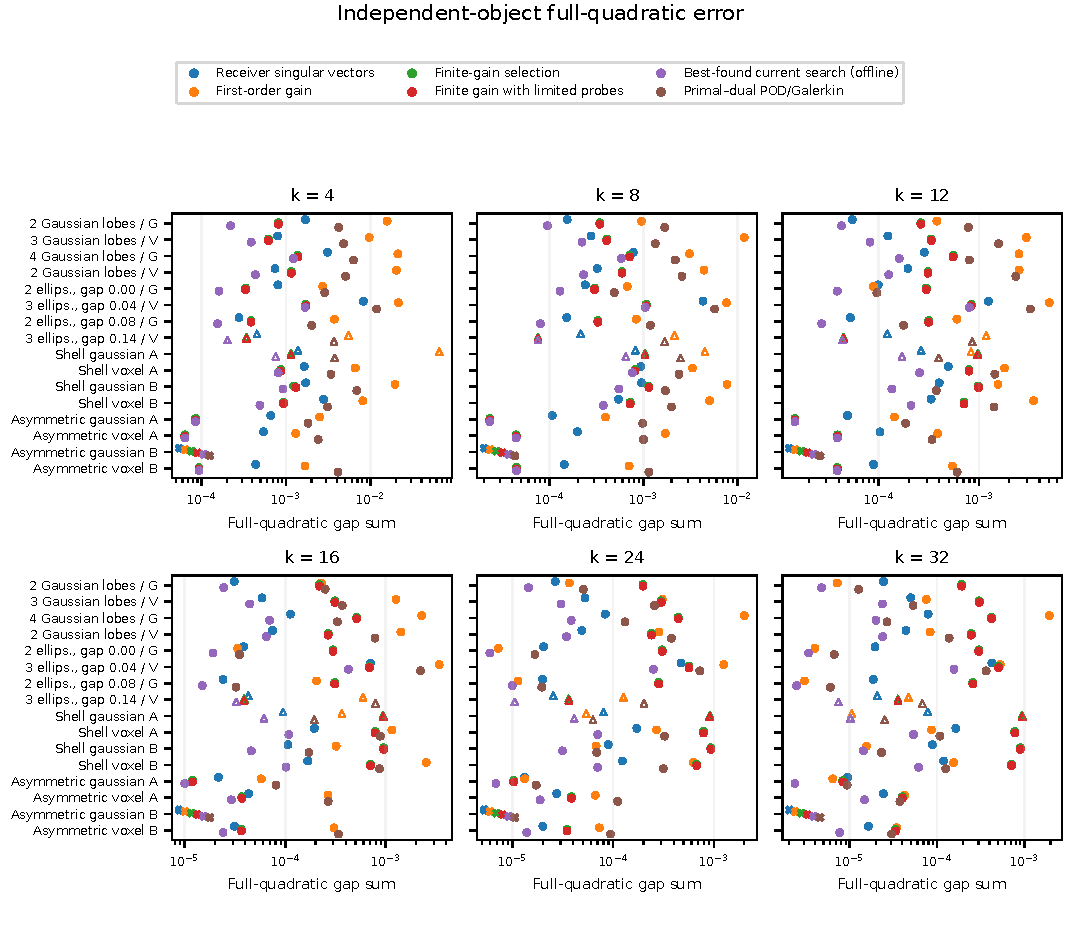
\includegraphics[width=.98\linewidth]{figures/current_design/02_object_fullgap.pdf}
\caption{Observed absolute full-quadratic gaps at all six budgets and all 16 planned objects. Filled/open markers distinguish complete/partial state coverage; missing objects have annotations rather than numerical zero. Object names describe geometry and material representation. Different objects are not points along one physical trajectory.}
\end{figure}
\begin{figure}[htbp]\centering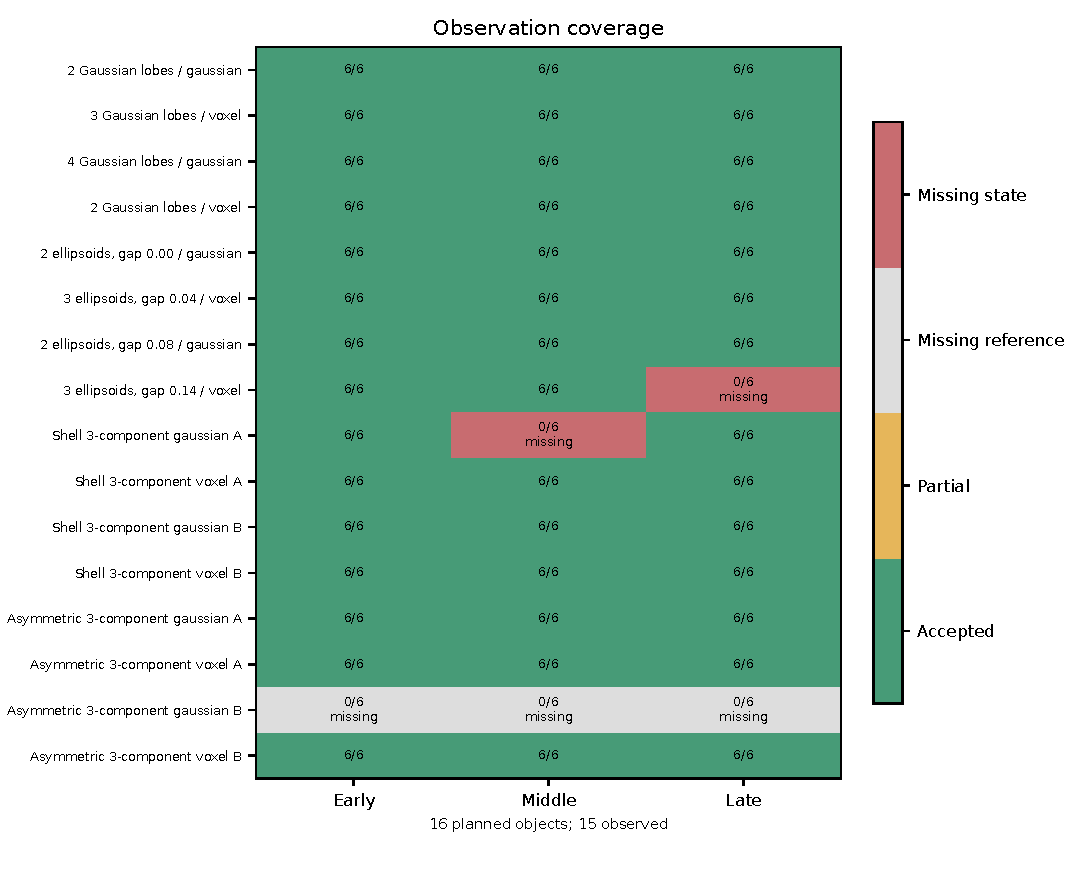
\includegraphics[width=.92\linewidth]{figures/current_design/04_zero_coverage.pdf}
\caption{Every planned noiseless state remains visible, including the failed reference and native process gaps. This conditional 43/48-state coverage does not close the original noise-inclusive gate.}
\end{figure}

\section*{S26. Information, cost and provenance boundaries}
The complete shared attempt ledger contains 166 uniquely paired starts/ends and 92629.937324\,s occupation (25.730538\,h), including diagnostics, full references, offline evaluation, failed attempts and interrupted work. Eight optimized continuation jobs consume 9086.047\,s. Five use CUDA candidate batches with CPU work retained; three small Gaussian cases use the exact CPU scoring path. Occupation includes host algebra, transfers, saving and waiting within a numerical job; it is not GPU kernel-active time.

\begin{figure}[htbp]\centering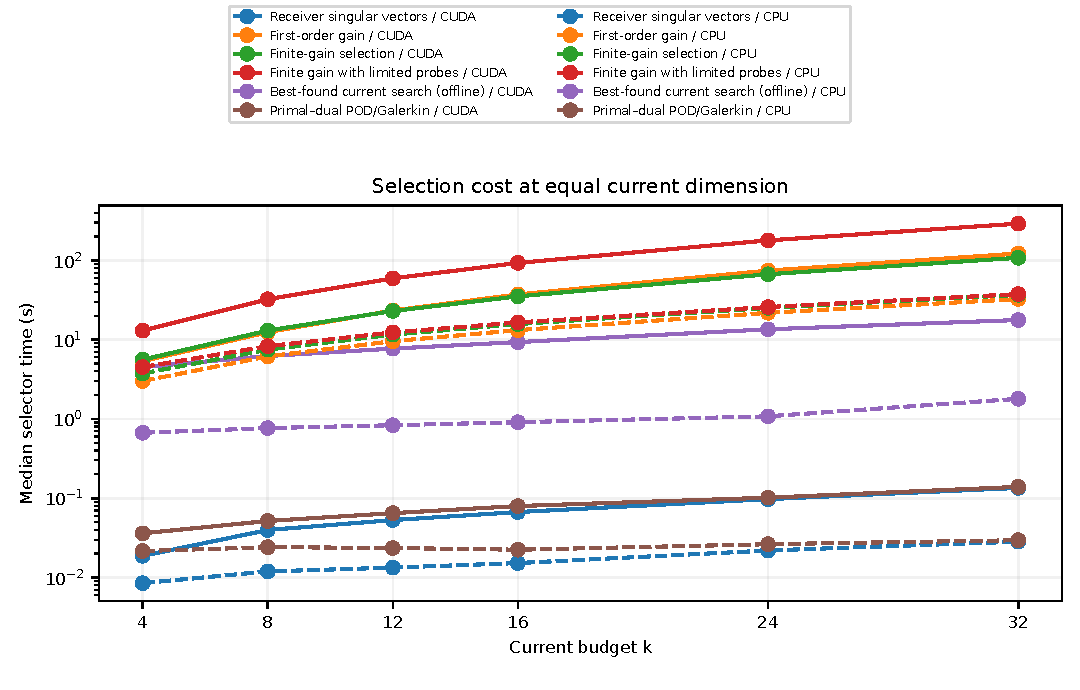
\includegraphics[width=.98\linewidth]{figures/current_design/03_selector_wall.pdf}
\caption{Version-separated shared-workspace marginal selector fees. The five CUDA-batched and three exact-CPU cases differ in object and material dimension, so these curves do not establish a cross-backend speedup. The older backend is not uniformly recorded and remains in the cost tables. Common-bank construction, reference, offline and interrupted work are separately charged; natural cold-deployment time is unmeasured.}
\end{figure}

The interrupted state retains 218 partial files and its uncertain-exit occupation upper bound of 1376.604324\,s. Failed native/reference attempts remain paid. All 46 core-validation source declarations match; seven of 15 earlier development declarations have an open historical source-version gap. One failed late-state setup component is missing, but its attempt fee is present. Cold/no-history/minimal-natural totals are unmeasured. Overlapping counter views are not summed twice.

The terminal archive binds old/optimized outputs, locks, configuration, material bases, reference authorities and attempts. Its SHA256 is
\par\noindent{\footnotesize\ttfamily ce31e9104fd25589207ee50e84dce9973525b39db0c991d20695ae82bab0e130}\par
Original seals and the external pre-first-selection authority for two unused references are retained with native/local mappings. Old records remain unchanged. Original SOM/TSOM/FFT-TSOM/S-DBIM publication-source gaps stay open.

Overall risk, cross-family/budget benefit, object wins and oracle capture fail their aggregate criteria. Only the adapted primal--dual comparison meets its conditional numerical threshold. Large-grid causal interventions, noise checks and selector reconstruction have no new results. The paper retains its mechanism and design-condition positioning.


\clearpage
\section*{S27. Receiver-centered exchange: frozen contract and dictionary}
\subsection{Receiver-centered conditional exchange protocol}
We use two development geometries, a near-contact object with Gaussian material coordinates and a layered object with voxel coordinates. A fixed extension uses a smooth Gaussian object and an asymmetric multi-object voxel target. Each supplies the initial, third-update, and seventeenth-update linearizations, with shared complex current dimensions $k=4,8,16$. The four objects therefore give 36 correlated state--budget cells. All reuse existing noiseless trajectories; states and budgets are not independent objects.

At each state a declared dictionary combines 32 receiver directions, 32 internal-propagation directions, 32 Fourier directions, 32 reduced primal--dual directions, 16 residual-current directions, and ten seeded random currents. Its 154 atoms have a lossless common embedding of rank 128. That embedding caches $L,S,B$ projections; the retained model still has exactly $k$ columns. This is a newly declared dictionary, not the original selector experiment's dictionary. The 1-swap teacher enumerates all feasible replacements in this domain: 600, 1168, and 2208 at the receiver starting spaces for $k=4,8,16$. It is a complete local enumeration, not a global optimum over all current subspaces.

The online proposal uses twelve incoming atoms, balanced across source families without complete-objective labels, and considers each deletable logical atom. It computes endpoint steps and reduced-anchor gains from a separate 64-column model. It then checks at most two finalists by the complete directional formula, accepts a resolved positive gain, and recomputes the conditional neighborhood. At most three actions are accepted. The exact-score teacher, unchecked surrogate, verified proposal, unchanged receiver, and a deletion/addition/swap policy with rank at most $k$ are recorded separately. A fixed restricted 2-swap domain supplies interaction diagnostics. Singular common cores trigger direct endpoint evaluation; endpoint stability determines feasibility.

The material state, full forward residual, injection, prior term $\ell$, damping, and physical coordinates are common to all methods. Full Jacobians and full-reference optimal steps are used only for offline diagnostics. Gaussian spaces have 54 real material coordinates; voxel spaces have 3456. The former allow complete information spectra, while voxel information diagnostics use sixteen fixed common directions. The material scale is $P=10^{-5}I$, separately recorded from LM damping. No measured noise covariance is fitted.

The reported risk is the complete frozen-quadratic gap relative to the paid reference solve. Its reference residual and floating-point floor accompany every cell. Ratios first sum paired risks within each object and only then aggregate objects. The numerical acceptance tolerance is predeclared; it is not a rigorous output-error bound. Selector construction, rejected candidates, failed factorizations, directed RHS, teacher labels and information diagnostics have separate cost records.

The twelve state runs yield 36 cells and 180 terminal policy records: unchanged receiver, reduced-anchor conditional exchange, exact-score local teacher, directed-verified exchange, and rank-at-most-$k$ actions. Early, middle, and late denote saved indices 0, 3, and 17. These are four reused objects, not a new independent acquisition dataset. No additional noise or nonlinear reconstruction trajectory is generated. The exchange dictionary is newly frozen and differs from the earlier broad current-selection search, including its random seed; their oracle domains are not interchangeable.

The declared dictionary contains 154 atoms: 32 receiver, 32 internal, 32 Fourier, 32 anchor primal/dual, 16 residual, and 10 random. Its lossless projected union has dimension 128. Each selected endpoint is a genuine current space with the stated complex dimension, shared across all illuminations. A conditional round removes one declared current atom and considers feasible replacements in the remaining shared core. Every accepted action reconstructs the endpoint step and the next conditional neighborhood. The local teacher examines its complete declared one-swap neighborhood, but follows at most three greedy actions; it is not a global current-space oracle.

\section*{S28. Finite gain, uncertainty, and acceptance}
Let $x=s_o$, $d=s_n-s_o$, $u=r+Jx$, and $z=Jd$. Expanding the unchanged complete quadratic gives
\[
Q=-u^Tz-(\ell+\Lambda x)^Td
-\tfrac12(z^Tz+d^T\Lambda d).
\]
This formula needs no complete adjoint once $Jx$ is available. Cached $Jx$ is updated after acceptance. Each new finalist still pays for the full physical direction action $Jd$.

Suppose certified output bounds give $\|u-\hat u\|\le e_u$ and $\|z-\hat z\|\le e_z$, while $d,\ell,\Lambda$ are fixed and evaluated exactly at this level. Cauchy--Schwarz and the quadratic expansion give
\[
|Q-\hat Q|\le e_u\|\hat z\|
+(\|\hat u\|+\|\hat z\|)e_z
+e_ue_z+\tfrac12e_z^2.
\]
Additional material or arithmetic errors need their own terms. An iterative residual without an applicable resolvent or output bound does not provide $e_u,e_z$. The present implementation consequently stores a null deterministic radius and uses high-fidelity numerical checks. The 22 unresolved and 14 move-budget stops remain distinct from a complete-neighborhood certificate.

The scale-aware numerical acceptance threshold is frozen before extension. The previous draft's approximate literal was corrected to its original exact declaration before the extension, with all 14792 existing classifications unchanged. This is recorded as a source epoch, not retroactively assumed from a current hash.

\section*{S29. Separate displacement from its evaluation}
The old-curvature displacement is
\[
v=-H_o^{-1}(J_o^TDs_o+D^Te_o),
\]
whereas the executed endpoint displacement includes the $D^TDs_o$ term and uses $H_n^{-1}$. On the same twelve-incoming candidate set at each receiver checkpoint, the diagnostic crosses direction choice ($v,d$) with linear or quadratic evaluation. All eight ranking rules execute the actual endpoint $d$; reference choice is additionally anchor or complete.

\begin{table}[htbp]\centering\caption{Mandatory top-one choices with negative actual complete gain, out of 36. No-op is excluded from this ranking diagnostic but is included in deployment acceptance.}
\begin{tabular}{@{}lrrrr@{}}\toprule
Reference&$v$, linear&$v$, quadratic&$d$, linear&$d$, quadratic\\\midrule
Complete&24&18&29&1\\
Richer reduced anchor&26&20&30&2\\\bottomrule
\end{tabular}\end{table}
These counts isolate a common-checkpoint finite-displacement effect. They do not identify the contribution of curvature alone to earlier entire-path policy ratios.

\section*{S30. Information magnitude, fidelity, and signed alignment}
All metrics use common real physical material coordinates and fixed $P=10^{-5}I$, separately from numerical LM damping. For $K_U=P^{-1/2}J_U^TJ_UP^{-1/2}$,
\[
\mathcal D(U)=\tfrac12\log\det(I+K_U),\qquad
d_{\rm eff}(U)=\operatorname{tr}[(I+K_U)^{-1}K_U].
\]
Complete spectra use the 54-dimensional Gaussian tangent. Voxel spectra use the same sixteen-direction projected material space. The projected spectrum cannot certify the 3456-dimensional voxel spectrum. Data normalization is numerical, without a calibrated covariance or a posterior-information claim.

The information subset fixes twelve incoming directions for each removal and adds the teacher-best endpoint when absent. The latter addition is utility-biased. The 3665 spectral records and the multiple-metric witness records are not independent physical samples or the entire exchange neighborhood.

The resolved information/utility witness increases $\mathcal D$ by 6.3127257611 and $d_{\rm eff}$ by 1.8613056862, while $Q=-5.5753875177\times10^{-5}$. Its initial gap $1.49684869697\times10^{-4}$ becomes $2.05438744875\times10^{-4}$. Its normalized curvature-fidelity improvement is $1.54242633\times10^{-4}$. The saved arrays, state/pool hashes, and move identity bind this example across spectral and action records.

All six complete Gaussian references have zero directions with $\nu\le1$ under the declared scale; each early state has two intermediate directions and 52 strong directions, and each middle/late state has 54 strong directions under the frozen bands. A direction decomposition using the matched full solve curvature reproduces the 72 endpoint risk changes with maximum relative discrepancy $6.50\times10^{-11}$. LM is retained in the matching risk weights rather than silently added to the information definition. No full-material weak-space claim is made for voxel.

\section*{S31. Costs, timing controls, and bounded learned priority}
Seventeen closed remote attempts cost 4889.515~s including all failures, teacher evaluations, diagnostics, and timing work. Two failed attempts cost 16.906~s and 1.062~s, respectively: a missing output directory in the initial CUDA gate and a platform-specific source-manifest locator before physics. Both failures and their receipts are preserved. The sampled device-memory maximum is 1872~MiB. There is no outstanding attempt, numerical process, or execution lock at the terminal snapshots.

The matched physical timing driver constructs one full state per representative object and performs actual CUDA FP64 direction actions. Forty-five formal and nine paid prewarm samples per object give five rotated repetitions of three methods at each current rank. Formal repetition measures timing variability, not independent scientific evidence. Each object pays 1656 tangent RHS across all 54 trials: 1008 in selection and 648 in separate offline endpoint evaluation. A fresh physical state costs 5.434~s and 5.727~s; historical anchor/pool acquisition and transferred arrays are separately receipted. Independent end-to-end cold time remains null.

\begin{table}[htbp]\centering\caption{Median warm physical selector time in seconds. Legacy is a receiver-start cached fixed-onepass control, not the entire earlier finite-gain policy.}\label{tab:exchange-time-supp}
\begin{tabular}{@{}llrrr@{}}\toprule
Material space&Policy&$k=4$&$k=8$&$k=16$\\\midrule
Gaussian&Cached one-pass&.138&.113&.151\\
&One directed decision&.328&.503&.937\\
&Conditional, at most three&.594&1.418&2.690\\
Voxel&Cached one-pass&.196&.207&.219\\
&One directed decision&.333&.596&1.215\\
&Conditional, at most three&.891&1.153&3.400\\\bottomrule
\end{tabular}\end{table}
The legacy Gaussian rank-16 control has measured negative complete gain $-2.1689\times10^{-7}$; this observation is retained. Shared setup is not silently renamed a cold measurement. Timing endpoint steps match production compatible outputs to relative error at most $6.73\times10^{-14}$. Production Gaussian small solves use CPU, whereas the matched physical backend uses CUDA; their wall times are not merged.

The priority pilot trains two fixed small architectures with three seeds each, using near-contact and layered objects for training, smooth for validation, and asymmetric for testing. The dataset contains 47712 dictionary records, of which 43108 are feasible. MLP heldout top-two capture is .988459, .988461, and .991617; the group-mean architecture gives .765571, .759893, and .980288. The analytical anchor top-two rule gives .998850. All six runs are retained. Total CPU training takes 9.413~s; these times exclude physical feature acquisition and new validation. No all-in network speedup or reconstruction contribution is established.

\section*{S32. Runtime provenance and release boundaries}
The terminal extension snapshot contains the executed state results and source; the subsequent timing snapshot is a delta bound to that full snapshot and unchanged core hashes. Runtime receipts identify actual module paths, source epochs, precision, and input hashes. Source changes are limited to the recorded implementation epochs; timing does not alter the core selector.

The public release byte-copies eligible executable sources and numeric archives. Metadata-only locator remaps carry original/public hashes and exact transformation records; no whole-source regular-expression privacy substitution is used. Forty-two historical vendor modules remain externally identified by hash. The release therefore supports evidence inspection, figure reproduction, and independent portable algebra tests, but is not a self-contained GPU Maxwell replay package.

An all-failed current/Schur batch can return before recording its phase-specific timer. Complete job wall time and failure counters remain charged. This branch was not triggered in the accepted timing snapshots and remains an implementation accounting limitation, rather than a demonstrated missing total fee. Private kernel transfers lack full byte instrumentation. Missing cold and transfer quantities retain null values and explicit reasons.

\end{document}
